% !TEX TS-program = xelatex
% !TEX useTabsWithFiles
% !TEX tabbedFile{classifying-stars/classifying-stars.tex}
% !TEX tabbedFile{hydrostatic-balance/hydrostatic-balance.tex}
% !TEX tabbedFile{mean-free-path/mean-free-path.tex}
% !TEX tabbedFile{stellar-atmospheres/stellar-atmospheres.tex}
% !TEX tabbedFile{atomic-lines/atomic-lines.tex}
% !TEX tabbedFile{degeneracy/degeneracy.tex}
% !TEX tabbedFile{convection/convection.tex}
% !TEX tabbedFile{nuclear-burning/nuclear-burning.tex}
% !TEX tabbedFile{main-sequence/main-sequence.tex}
% !TEX tabbedFile{post-main-sequence/post-main-sequence.tex}

\documentclass[profonts,stix,symmetric]{astro-bookshelf}
\hypersetup{colorlinks=true,linkcolor=blue,citecolor=black,urlcolor=blue}

\setcounter{secnumdepth}{1}

\graphicspath{%
{frontmatter/}{classifying-stars/figs/}{hydrostatic-balance/figs/}{mean-free-path/figs/}{stellar-atmospheres/figs/}{atomic-lines/figs/}{degeneracy/figs/}{convection/figs/}{nuclear-burning/figs/}{main-sequence/figs/}
}

\usepackage{starType}
% symbols used in this work
\newcommand*{\ssb}{\ensuremath{\sigma_{\mathrm{SB}}}} %Stefan-Boltzmann constant
\newcommand*{\rn}{\ensuremath{r_{\mathrm{N}}}} %nuclear radius
\newcommand*{\re}{\ensuremath{r_{\mathrm{E}}}} %classical turning point
% \newcommand*{\EG}{\ensuremath{E_{\mathrm{G}}}} %Gamow energy
% \newcommand*{\Epk}{\ensuremath{E_{\mathrm{pk}}}} %Peak energy for reaction
\newcommand*{\TPstar}{\left.\frac{\dif T}{\dif P}\right|_{\star}} % derivative of T wrt P in star
\newcommand*{\sun}{\ensuremath{\odot}} %sun
\newcommand*{\eF}{\ensuremath{\varepsilon_{\mathrm{F}}}} %Fermi energy

% vector macros
\newcommand*{\unitvector}[1]{\ensuremath{\bvec{\hat{#1}}}}
\newcommand*{\unitn}{\unitvector{n}} %unit 'n' vector
\newcommand*{\unitk}{\unitvector{k}} %unit 'k' vector
\newcommand*{\unitj}{\unitvector{\jmath}} %unit 'j' vector
\newcommand*{\vu}{\ensuremath{\bvec{u}}} %vector 'u'
\newcommand*{\vv}{\ensuremath{\bvec{v}}} %vector 'v'
\newcommand*{\vx}{\ensuremath{\bvec{x}}} %vector 'x'
\newcommand*{\vr}{\ensuremath{\bvec{r}}} %vector 'r'
\newcommand*{\vg}{\ensuremath{\bvec{g}}} %vector 'g'
\newcommand*{\vp}{\ensuremath{\bvec{p}}} %vector 'p'
\newcommand*{\vk}{\ensuremath{\bvec{k}}} %vector 'k'
\newcommand*{\vkt}{\ensuremath{\bvec{k}_{t}}} %vector 'k_{t}'
\newcommand*{\vxi}{\ensuremath{\bvec{\xi}}} %vector 'k'
\newcommand*{\usp}{\unitskip}
\newcommand*{\nsp}{\usp}
\newcommand*{\watt}{\unitstyle{W}}

\newcommand*{\pfcn}{\ensuremath{\mathcal{Q}}}
\newcommand*{\EG}{\ensuremath{E_{\mathrm{G}}}}
\newcommand*{\Epk}{\ensuremath{E_{\mathrm{pk}}}}


% for aligning table columns
\usepackage{dcolumn}
\newcolumntype{d}[1]{D{.}{.}{#1}}
\newcommand{\tabhead}[1]{\multicolumn{1}{c}{#1}}
% for coloring rows
\usepackage{colortbl}
\usepackage{aasjournals}

\newcommand*{\maintitle}{Stars}
\newcommand*{\notice}{\thanks{\ccCopy\ 2017 Edward Brown; \ccbyncsa\ Except where explicitly noted, this work is licensed under the Creative Commons
Attribution-NonCommercial-ShareAlike 4.0 International (CC BY-NC-SA
4.0) license.}}

\title{To Build A Star}
\publisher{Open Astrophysics Bookshelf}
\author{Edward Brown}
\date{26 September 2017}

\begin{document}
\frontmatter
\pagenumbering{roman}
% !TEX root = ../intro-stellar-physics.tex

\ThisCenterWallPaper{1.0}{cover-art}
\maketitle
\newpage
\begin{fullwidth}
\thispagestyle{empty}

\vspace{3\baselineskip}
\noindent \textit{About the cover:} The image shows the star field in the direction of the second closest star to Earth, Proxima Centauri.\\
\noindent Credit \& Copyright: David Malin, UK Schmidt Telescope, DSS, AAO

\vfill
\noindent \ccCopy\ 2017 Edward Brown\\
\noindent git version \input{git-info}\ldots

\vspace{3\baselineskip}
\noindent \ccbyncsa \\
\noindent Except where explicitly noted, this work is licensed under the Creative Commons
Attribution-NonCommercial-ShareAlike 4.0 International (CC BY-NC-SA
4.0) license.

\end{fullwidth}

\newpage
% !TEX root = ../intro-stellar-physics.tex

\section*{Preface}
These notes grew out of a collection of handouts and exercises that I wrote while teaching the junior/senior undergraduate course on stars at Michigan State University in the autumn semesters of 2012, 2014, and 2016. In addition to deriving a basic physical description of how stars work, a secondary goal of the course was to train students to make simple physical models and order-of-magnitude estimates. This is a crucial skill that is not incorporated enough into the typical undergraduate physics courses. In keeping with this goal, many of the exercises asked the students to make estimates or to employ simple models, such as constant density throughout the star, rather than to perform elaborate calculations.

Concern about rising costs motivated me during the spring and summer of 2018 to assemble the handouts and exercises into a package that could be inexpensively distributed to students and eliminate the need for a required textbook. As I prepared for the transition to online teaching in the spring and summer of 2020, I added notes on three common numerical tasks: finding roots, solving ordinary differential equations, and interpolating tabulated data. These methods are used in the group computational project that is part of my course. Because there are many excellent references and numerical libraries available for these tasks, the goal of the appendix is just to introduce the techniques.

\newthought{There are several options for the order in which to present material.} One would be to start with chapter~\ref{ch.basic-stellar-properties}, which covers hydrostatic equilibrium and establishes estimates for the mean stellar density, pressure, and temperature. The material in chapter~\ref{ch.starlight} on radiant intensity, flux, and thermal emission would then be introduced in chapters~\ref{ch.radiative-transport} and \ref{ch.classifying-stars}, which cover radiative heat transport in the stellar interior and the conditions at the photosphere. The remainder of chapter~\ref{ch.starlight} on magnitudes would then come later, perhaps in chapter~\ref{ch.main-sequence} where we discuss the main sequence.

Although this order is logical, after deliberation I decided on the layout used here for pedagogical reasons. First, radiative transfer is a difficult subject, and introducing the basic concepts early gives the students more time to become familiar with the topic. Second, finding Wien's law requires a numerical rootfind (exercise~\ref{ex.Wien-wavelength}), and this is a good warmup for further numerical projects. Finally, the discussion of radiative intensity allows us to introduce magnitudes and color indices, thereby making contact with the subject's observational foundations at the start.

\newthought{The text layout uses the \code{tufte-book} \LaTeX\ class}\sidenote{\url{https://tufte-latex.github.io/tufte-latex/}}. The main features are a large outer margin in which the students can take notes and the tight integration of text, figures, and sidenotes. Exercises are embedded throughout the text. The exercises range from comprehension checks to longer, more challenging problems. Some of the exercises have a numerical component, denoted with a ``\notebook'' symbol. Because the exercises are spread throughout the text, there is a ``List of Exercises'' in the front. I've also added boxes containing more advanced material that I felt students should be exposed to, but were not essential to the main development of the course. 

\newthought{One evening I tried to enliven the chapter titles.} I noticed that the first two chapters had titles that were also titles for pop songs. I then decided to find song titles that would fit for the remaining chapters. When selecting titles, I imposed a rule that they all could plausibly go together on a playlist. This was challenging since the chapters originally had titles such as ``The equation of state'' and ``The radiative opacity''. The credits for the chapter titles, in order, go to Muse, Queen/David Bowie, Greta van Fleet, Dio, Deep Purple, David Bowie, The Traveling Wilburys, and Muse.

\newthought{Please be advised that these notes are under active development.} To refer to a specific version of the notes, use the eight-character stamp labeled ``git version'' on the copyright page.


\tableofcontents
\listoffigures
\listoftables
\listofexercises
\listofsidebars


\mainmatter
\pagenumbering{arabic}
\setcounter{page}{1}

\chapter{Stellar Classification}\label{ch.classifying-stars}
% !TEX root = ../intro-stellar-physics.tex

\nocite{Mihalas1978Stellar-Atmosph,LeBlanc2010An-Introduction,Carroll2006An-Introduction}

To recap, we have established a description for the basic features of self-gravitating fluid:
\begin{enumerate}

\item For a set mass and radius, hydrostatic equilibrium (balance of pressure and gravity) is established on the time needed for a sound wave to cross the star. Once this equilibrium is established, the central pressure, density, and temperature are established.

\item The gradient in temperature from center to surface drives a luminosity, which is controlled by the opacity of material in the stellar interior.

\item The ambient pressure and temperature near the stellar photosphere (where $\tau \sim 1$) are set by the surface gravity and opacity.

\end{enumerate}

What we haven't---yet---established is how the luminosity is generated: if nuclear reaction are not operating, then the star must contract (on a Kelvin-Helmholtz timescale) until the central temperature is sufficiently hot for reactions to generate the required luminosity.
Before discussing this, however, we shall explore how the emergent spectra of stars serve as diagnostic indicators of ambient conditions in the stellar photosphere. 

\section{Overview}

If light from the Sun is passed through a grating (a piece of glass with finely etched lines), the light is dispersed in wavelength and creates a spectrum, such as the highly detailed one show in Fig.~\ref{f.solar-spectrum}. 
\begin{marginfigure}
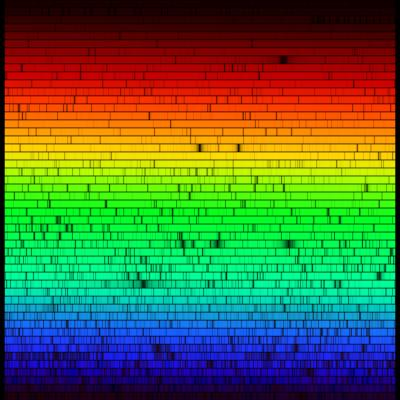
\includegraphics[width=\linewidth]{sunsqa}
\caption{\label{f.solar-spectrum} Visible spectrum of the Sun. Wavelength increases along a row from left to right, and by rows from bottom to top. \emph{Credit:
N.A.Sharp, NOAO/NSO/Kitt Peak FTS/AURA/NSF. Image copyright }}
\end{marginfigure}
Superposed on the slow variation from red to violet are dark \newterm{absorption lines}. These are caused by absorption of photons at specific frequencies by ions, atoms, and molecules in the solar atmosphere.

Beginning in the late 1800's, astronomers began classifying stars by the observed absorption lines in the spectra. At this time, Edward Pickering and Williamina Fleming of the Harvard College Observatory began amassing a vast catalog of stellar spectra. They classified these spectra according to the strength of observed hydrogen Balmer lines (the first four are H$\alpha$: \val{657}{\nano\meter}; H$\beta$: \val{486}{\nano\meter}; H$\gamma$: \val{434}{\nano\meter}; H$\delta$: \val{410}{\nano\meter}). Stars, such as Vega, with the strongest Balmer lines were classified as type ``A'', those with the next strongest were type ``B'', and so forth. In Annie Jump Cannon, who had joined the group in 1896 and would later succeed Fleming as curator of astronomical photography at the observatory, simplified and reorganized the scheme, and added decimal subdivisions ($0\ldots9$) for each type\sidenote{For example, the Sun's type is G2}. When stellar color is taken into account, the ordering of stars, from blue to red, is ``OBAFGKM''. In the 1990's the ``L'' and ``T'' classes were added\cite{Kirkpatrick1999Dwarfs-Cooler-t} for cool stars and brown dwarfs (stellar-like objects that do not reach central temperature sufficient for fusion of hydrogen into helium).

Hertzsprung and Russell independently noticed that most stars tended to lie along a band, termed the \newterm{main sequence} in a plot of absolute magnitude (or luminosity) against stellar type (now known as a \newterm{Hertzsprung-Russell diagram}). Figure~\ref{f.HR} shows some standard main-sequence stars, along with their stellar type and approximate color.
\begin{marginfigure}
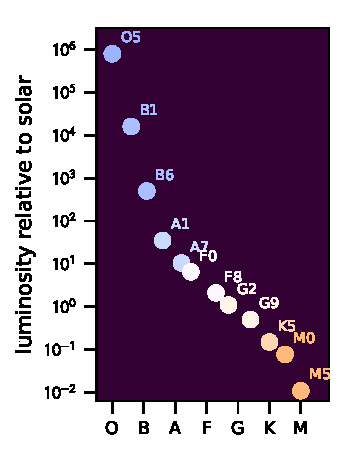
\includegraphics[width=\linewidth]{HR}
\caption{\label{f.HR} Hertzsprung-Russell diagram showing standard main-sequence stars. Colors are approximate translations of the spectra.}
\end{marginfigure}

In an influential PhD thesis, Cecilia Payne-Gaposhkin\cite{Payne1925Stellar-Atmosph} applied the Boltzmann and Saha equations to show that different stellar spectra were consistent with changes in temperature, rather than composition, of the stellar photosphere. The sequence of stellar types is therefore a temperature sequence, with ``O'' stars being the hottest. 

\section{The hydrogen atom}

To understand why the Balmer lines are strongest in a certain range of temperatures, we first need to review the workings of a hydrogen atom.

The electrons bound to an atom or molecule can only occupy states having a discrete set of energies. For example, the electron in a hydrogen atom only has energies
\begin{equation}\label{e.H-levels}
        E_{n} = -\val{13.6}{\eV}\times \frac{1}{n^{2}},
\end{equation}
where $n > 0$ is an integer known as the principal quantum number.  These energies are negative, relative to a free electron.  For example, the ground state ($n=1$) has energy $\ERy = -\val{13.6}{\eV}$, meaning that it takes \val{13.6}{\eV} to remove an electron in its ground state from the atom.

Because the electrons in an atom can only have certain energies, the atom can only absorb or emit light at specific wavelengths, such that the energy of the photon matches the difference in energy between two levels. For example, a hydrogen atom in its ground state can absorb a photon of energy
\[
        E_{1\to2} = -\ERy \left(\frac{1}{2^{2}} - \frac{1}{1^{2}}\right)
                 = \val{10.2}{\eV}
\]
corresponding to the energy required to move the electron from $n=1$ to $n=2$. The wavelengths that can be absorbed by a hydrogen atom at rest can be found by substituting $E = hc/\lambda$ into equation~(\ref{e.H-levels}):
\begin{equation}
        \lambda_{m\to n} = \lambda_{0}\left(\frac{1}{n^{2}}-\frac{1}{m^{2}}\right)^{-1},
\end{equation}
where $\lambda_{0} = \val{91.2}{\nano\meter}$ and $n > m$.
The transitions to the lowest levels are named after their discoverers: Lyman for $m\to1$, Balmer for $m\to2$, Paschen for $m\to3$. A greek letter is used to denote the higher state: for example Lyman $\alpha$ (abbr.\ Ly$\alpha$) means $2\to1$, with $\lambda_{\mathrm{Ly}\alpha} = \val{121.6}{\nano\meter}$.  The first line transition in the Balmer series is $3\to2$, and is designated H$\alpha$: $\lambda_{\mathrm{H}\alpha} = \val{656.3}{\nano\meter}$. The first 20 lines for the Lyman ($m\to1$), Balmer ($m\to2$), and Paschen ($m\to3$) are shown in Fig.~\ref{f.H-spectrum}; note the $4\to3$ transition is outside the plot range. The Balmer lines lie in the visible range. Note that $\lambda_{m\to n} < \lambda_{0}$; photons with wavelengths $\lambda < \val{91.2}{\nano\meter}$ have sufficient energy to knock the electron out of the atom, thereby producing a hydrogen ion and a free electron.

\begin{marginfigure}[-8\baselineskip]
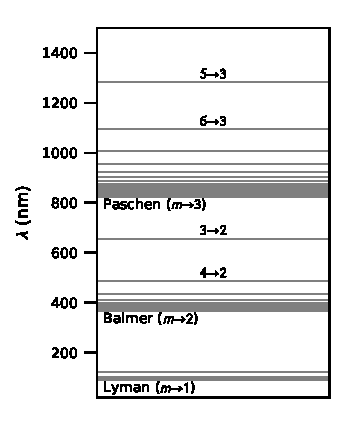
\includegraphics[width=\linewidth]{H-spectrum}
\caption{Spectral lines of neutral hydrogen. 
\label{f.H-spectrum}}
\end{marginfigure}

\section{The Boltzmann Equation}
\label{s.boltzmann-eqn}

In order to produce a Balmer absorption line, we must have some hydrogen atoms in the photosphere with electrons in the energy level $n=2$. The more atoms with $n=2$, the more absorption and the stronger the line. To find the number of atoms with energy level $n=2$, we make use of a fundamental result, due to Boltzmann, from statistical (thermal) physics; namely, that if our sample of atoms is in thermal equilibrium, then the ratio of the number of atoms with energy $E_{i}$ to the number of atoms with energy $E_{j}$ is
\begin{equation}\label{e.boltzmann}
\frac{N_{i}}{N_{j}} = \frac{g_{i}}{g_{j}} 
\exp\left(-\frac{E_{i}-E_{j}}{\kB T}\right).
\end{equation}
Here the number $g_{n}$ gives the number\sidenote{$g_{n}$ is known as the \emph{degeneracy} of a given level $n$} of quantum mechanical states having energy $E_{n} = -\ERy/n^{2}$. For an energy level $n$, there are $n^{2}$ possible states, each having a different angular momentum. For each of these $n^{2}$ states, both the electron and proton may each have 2 possible spins. The total number of states for energy $E_{n}$ is therefore $g_{n} = 2\times2\times n^{2}$.

Suppose we wish to know the fraction of atoms in a given state $i$: that is, we want to know
\[	x_{i} = \frac{N_{i}}{N_{1}+N_{2}+\ldots+N_{i}+\ldots} ? \]
Using equation~(\ref{e.boltzmann}), we can express $x_{i}$ as 
\begin{eqnarray}
  x_{i} &=& \frac{g_{i}e^{-E_{i}/\kB T}}{g_{1}e^{-E_{1}/\kB T}+g_{2}e^{-E_{2}/\kB T}+\ldots+g_{i}e^{-E_{i}/\kB T}+\ldots} \nonumber\\
        &\equiv& \frac{g_{i}e^{-E_{i}/\kB T}}{\pfcn}.
\end{eqnarray}
The quantity 
\begin{equation}\label{e.partition-function}
	\pfcn = \sum_{n} g_{n}\exp\left(-\frac{E_{n}}{\kB T}\right)
\end{equation}
is called the \emph{partition function}: loosely speaking, it indicates the number of ways the sample of atoms can be partitioned among the different energy levels.

\begin{exercisebox}[Partition function for neutral hydrogen]
Assuming that the first term $g_{1}e^{-E_{1}/\kB T}$ dominates the sum in the partition function (see Box~\ref{sb.partition-function}), plot the fraction of neutral hydrogen in its $n=2$ state as a function of temperature, for $\val{5\,000}{\K} < T < \val{20\,000}{\K}$.
\end{exercisebox}

\begin{sidebar}[The partition function for neutral hydrogen]
\label{sb.partition-function}
The partition function for neutral hydrogen, eq.~(\ref{e.partition-function}), has some interesting features. Substituting $g_{n}=4n^{2}$ and $E_{n} = -\ERy/n^{2}$ and factoring out common terms gives,
\[	\pfcn = 4e^{\beta\ERy}\sum_{n} n^{2} e^{-\beta\ERy(1-1/n^{2})}. \]
Here we have used the shorthand $\beta = (\kB T)^{-1}$. Written in this fashion, it is clear that for $n\gg 1$, the sum diverges, since the individual terms go as $n^{2}e^{-\beta\ERy}$ as $n\to\infty$. In practice, this isn't a problem, as there is an upper limit on $n$ set by ambient conditions. For example, the mean distance of the electron from the nucleus is $\approx \abohr n^{2}$, where $\abohr = \val{\sci{5.29}{-11}}{\cm}$ is the Bohr radius. As a result, each atom takes up a volume $\approx \abohr^{3}n^{6}$; if we want the atoms to not overlap, then the volume per atom, $V/N = 1/xi$, must be larger than this by some factor. Suppose we set that the volume of an atom must be less than half of that available in our gas; then
\[
\xi = \frac{N}{V} < \frac{N}{N\cdot 2\abohr^{3}n^{6}}.
\]
Thus the maximum level is $n < (2\abohr^{3}\xi)^{-1/6}$. For a typical A-star photospheric density $\xi\sim \val{10^{15}}{\cm^{-3}}$, the density cutoff is $n \lesssim 35$. In practice the cutoff will be even lower.

The precise maximum value of $n$ is not that important for most applications. The reason is that the in the partition function increase only slowly. For example, at $T=\val{10^{4}}{\K}$, the terms and cumulative sum in the partition function are as follows.
\begin{center}
\begin{tabular}{rrr}
$n$ & $n^{2} e^{\beta\ERy(1-1/n^{2})}$ & $4\sum_{i=1}^{n} i^{2}e^{-\beta\ERy(1-1/i^{2})}$ \\
\hline
   1 & 1.00e+00 &  4.0000 \\
   2 & 2.88e-05 &  4.0001 \\
   3 & 7.23e-06 &  4.0001 \\
  \multicolumn{3}{c}{\vdots} \\
  26 & 9.62e-05 &  4.0038 \\
  \multicolumn{3}{c}{\vdots} \\
  52 & 3.78e-04 &  4.0274 \\
  \multicolumn{3}{c}{\vdots} \\
 268 & 9.99e-03 &  7.5901 \\
\end{tabular}
\end{center}
As we can see from the cumulative sum (rightmost column), the partition function is insensitive to the precise value of the cutoff; indeed, it is reasonably accurate to just use the first term, $Q\approx 4e^{\beta\ERy}$. 
\end{sidebar}

\section{Ionization: The Saha equation}
\label{s.saha-eqn}

As the temperature in the gas rises, there are more photons with sufficient energy to eject electrons from an atom. In addition, collisions between atoms also become sufficiently energetic to ionize the atom. In astronomical nomenclature, the ionization state is denoted by a small Roman numeral: \ion{Fe}{i} denotes neutral iron, \ion{Fe}{ii} denotes singly-ionized iron (charge $+1$), \ion{Fe}{iii} denotes doubly-ionized iron (charge $+2$), and so on. In thermal equilibrium, the rate at which atoms are ionized must equal the rate at which ions and electrons recombine: for example, in a gas consisting of hydrogen atoms, hydrogen ions (i.e., protons), and electrons we have
\[
	\ion{H}{ii} + e \longleftrightarrow \ion{H}{i}
\]


We'd like to extend equation~(\ref{e.boltzmann}) to find the ratios of two ionization states $N\,(i+1)/N\,(i)$.  


What we will do is look at the equation for this ratio, known as the \emph{Saha equation}, and try to understand how it works.  The Saha equation for the ratio of ionized to neutron hydrogen is
\begin{equation}\label{e.saha}
\frac{N\,\textrm{\scshape ii}}{N\,\textrm{\scshape i}} 
= {\color{red}\left[\frac{2}{n_{e}}
\left(\frac{2\pi m_{e}kT}{h^{2}}\right)^{3/2}\right]}
\frac{\pfcn_{\mathrm{II}}}{\pfcn_{\mathrm{I}}} \exp\left(-\frac{E_{\mathrm{ion}}}{\kB T}\right).
\end{equation}
In this equation, $n_{e}$ denotes the electron density---the number of free electrons per unit volume---and $m_{e}$ is the electron mass.

Let us interpret equation~(\ref{e.saha}) in terms of eq.~(\ref{e.boltzmann}).  First, there is the factor $\exp(-E_{\mathrm{ion}}/\kB T)$. Here $E_{\mathrm{ion}}$ is the difference in energy between the ground states of the different ionization stages (for this example, $E_{\mathrm{ion}} = \val{13.6}{\eV}$).  That is just as in equation~(\ref{e.boltzmann}). To understand the factor $\pfcn_{\mathrm{II}}/\pfcn_{\mathrm{I}}$, consider that we are asking for the ratio between the total number of ionized atoms to the total number of neutral atoms; and this means summing over all of the states with electrons in different energy states. It is plausible, therefore, that the factor $g_{i}/g_{j}$ from equation~(\ref{e.boltzmann}) would be replaced by $\pfcn_{\mathrm{II}}/\pfcn_{\mathrm{I}}$.

In addition to the number of possible states for the ion, we need to allow for the number of possible electron states.  When the atom is ionized, each electron quickly acquires an average kinetic energy $(3/2)\kB T$. There are many different states with this energy: the electron can be in different locations, and moving in different directions.  At first, you might think that there would be an infinitude of possible electron states.  Quantum mechanics, however, sets limitations on the number of electron states.

First, we have the Pauli exclusion principle: no two electrons can be in the same location with the same momentum and same spin. What do we mean by same location and momentum?  Recall the Heisenberg uncertainty principle: the electrons $x$-position and $x$-momentum are spread about a range of values $\Delta x$ and $\Delta p_{x}$, and these uncertainties are related via
\[ \Delta x\,\Delta p_{x} \gtrsim h. \]
Thus, if we imagine dividing our volume into little boxes of volume
\[ 
 \Delta V = \Delta x\,\Delta y\,\Delta z \approx \frac{h^{3}}{\Delta p_{x}\,\Delta p_{y}\,\Delta p_{z}},
\]
each box can hold two electrons.\sidenote{Because electrons have spin 1/2, we can put two electrons into the same position and momentum state if their spins are oppositely directed.} Suppose we have a volume $V$; how many boxes are there?  The number of available boxes is
\[
	\frac{V}{\Delta V} \approx \frac{V\;\Delta p_{x}\,\Delta p_{y}\,\Delta p_{z}}{h^{3}}.
\]
To estimate the size of $\Delta p_{x}\,\Delta p_{y}\,\Delta p_{z}$, let's estimate $\Delta p_{x}\sim p_{x}$; further, if everthing is isotropic then $p_{x}\approx p_{y}\approx p_{z}$ on average, so $\Delta p_{x}\,\Delta p_{y}\,\Delta p_{z} \sim p_{x}^{3}$.  Now the kinetic energy of the electron is $p^{2}/2m_{e}$, and $p^{2} = p_{x}^{2} + p_{y}^{2} + p_{z}^{2} \approx 3 p_{x}^{2}$. Hence the kinetic energy is $(3/2)p_{x}^{2}/m_{e}$; in thermal equilibrium, however, the kinetic energy has an average value of $(3/2)\kB T$.  The value of $p_{x}^{2}$ is therefore
\[
	p_{x}^{2} \approx m_{e}\kB T,
\]
and the number of boxes is
\[
	\frac{V}{\Delta V} \sim V\frac{p_{x}^{3}}{h^{3}} \sim V\frac{\left(m_{e}\kB T\right)^{3/2}}{h^{3}}.
\]
If our volume $V$ contains $N_{e}$ electrons, then the number of boxes---which is the number of states---per electron is
\[
	\frac{2V}{N_{e}\Delta V} \sim \frac{2V}{N_{e}}\frac{\left(m_{e}\kB T\right)^{3/2}}{h^{3}}.
\]
The factor of 2 appears because each box can hold 2 electrons.  Recognizing that $N_{e}/V = n_{e}$, we see that this number of states per free electrons corresponds to the factor in $\color{red}\left[\;\right]$ in equation~(\ref{e.saha}). When the numerical calculation is done correctly, the additional factor of $2\pi$ arises.

\section{Classifying stars by spectra}

The Balmer lines, which correspond to transitions $2\to3$, $2\to 4$, \ldots, are most prominent in A stars. These stars have $\Teff = \valrng[--]{7\,500}{9\,500}{\K}$. At lower temperatures, the population of hydrogen atoms in the level $n=2$ decreases as $e^{-E_{2}/kT}$ and the lines become weak. At higher temperatures, the number of neutral hydrogen atoms decreases; most of the hydrogen is ionized, and the Balmer lines again become weaker.

These arguments apply to other species present in the stellar photosphere.  In the hottest stars (type O: $\Teff > \val{30\,000}{\K}$), hydrogen is mostly ionized and the lines are He\,\textsc{ii} and multiply-ionized metals. As temperature cool into the B and A series, the hydrogen lines increase in strength. Going from F into G ($\Teff = \valrng[--]{5\,000}{6\,000}{\K}$, the hydrogen lines decrease, while lines from singly-ionized and neutral metals such as Ca\,\textsc{ii}, Ca\,\textsc{i}, Fe\,\textsc{i} become strong.  At still lower temperatures in the K and M ($\Teff < \val{3\,500}{\K}$) types, absorption from molecules such as TiO becomes prominant.  An example is the broad trough seen in the K spectrum near $\lambda = \val{500}{\nano\meter}$ in Fig.~\ref{f.spectral-types}, which displays standard stellar spectra for selected types at optical wavelength.

\begin{figure}[hbp]
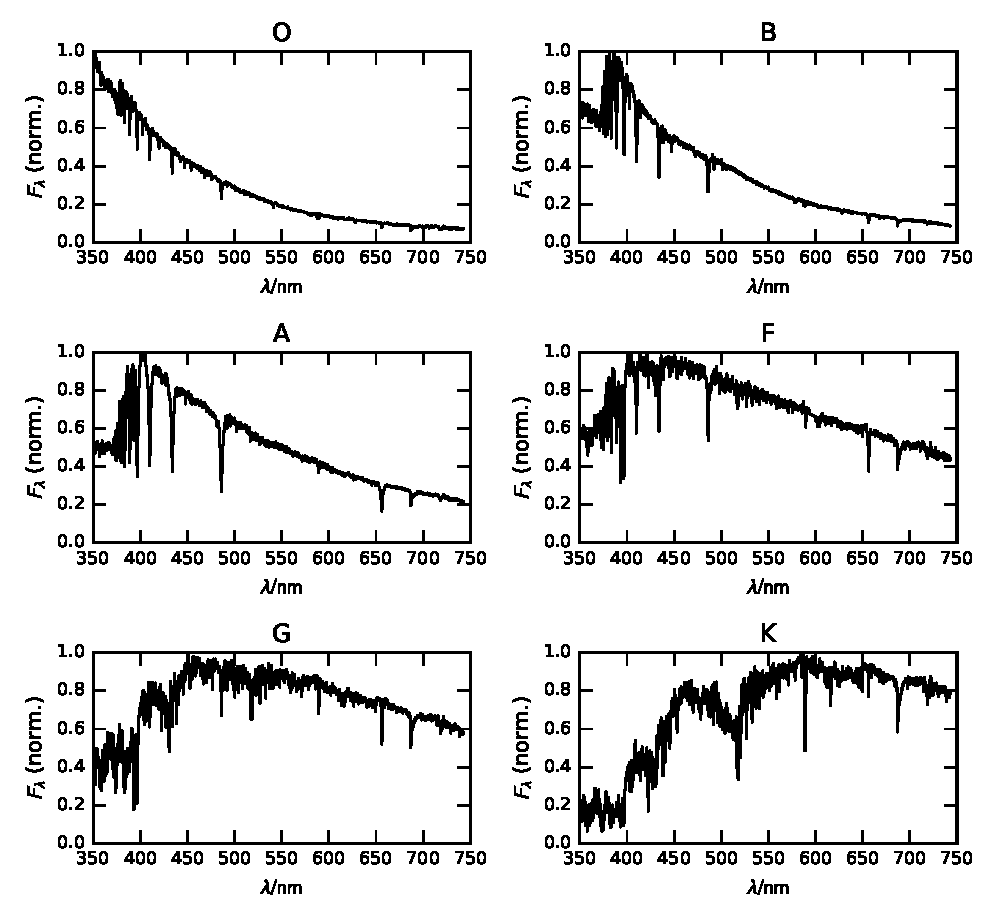
\includegraphics[width=\linewidth]{spectral_types}
\caption[Standard stellar types]{\label{f.spectral-types} Spectra from main-sequence stars of spectral types O--K. Data from \protect\citet{Jacoby1984A-library-of-st}.}
\end{figure}

As we have seen, the temperature of the stellar atmosphere determines which species are present and hence which lines are present. The width of the line conveys information about the pressure at the photosphere. To understand this, we need to digress briefly on the shape of the line.

\begin{sidebar}[The driven damped oscillator]
Let's begin with a simple system: a mass $m$ attached to a spring with force $F = -kx$.

\begin{center}
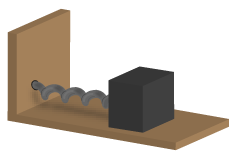
\includegraphics[width=0.5\linewidth]{simple-spring}
\end{center}

\noindent If we put the origin of our coordinate system where the mass is at rest with the spring relaxed, then the equation of motion of the mass is
\begin{equation}\label{e.SHO-basic}
	\DDtt{x} + \frac{k}{m} x = 0.
\end{equation}
You have solved this equation before: the most general solution is
\begin{equation}\label{e.SHO-general-solution}
	x(t) = x_{0}\cos(\wot) + \frac{v_{0}}{\omega_{0}}\sin(\wot)
\end{equation}
with $\omega_{0}^{2} = k/m$ and with $x_{0}$ and $v_{0}$ being the initial position and velocity of the mass. The angular frequency $\omega_{0}$ is related to the period of oscillation $T$ as $\omega_{0} = 2\pi/T$.

\newthought{Now let's push on our mass with an oscillating force, $F\cos(\omega t)$ with $\omega\neq\omega_{0}$.} A real world example would be holding a vibrating tuning fork near another fork tuned to a different frequency.  The equation of motion is now
\begin{equation}\label{e.SHO-driven}
	\DDtt{x} + \omega_{0}^{2}x = \frac{F}{m}\cos(\wt).
\end{equation}
You can verify by substitution that a general solution is
\[
	x(t) = \frac{F/m}{(\omega_{0}^{2}-\omega^{2})}\cos(\wt) + A\cos(\wot)+B\sin(\wot).
\]
Let's start with our harmonic oscillator at rest ($v_{0} = \left.\dif x/\dif t\right|_{t=0} = 0$) and at $\left. x\right|_{t=0} = 0$.  With these conditions, we can determine the constants $A$ and $B$; the solution is
\[
	x(t) = \frac{F/m}{(\omega_{0}^{2}-\omega^{2})}\left[\cos(\wt)-\cos(\wot)\right].
\]
Let's recast this by defining $\Delta = \omega_{0} - \omega$ and $\omega_{m} = (\omega_{0}+\omega)/2$.  Then
\begin{eqnarray*}
  \omega_{0}^{2}-\omega^{2} &=& (\omega_{0}-\omega)(\omega_{0}+\omega) = 2\Delta\omega_{m},\\
  \cos(\wot) &=& \cos\left(\wmt+\Delta t/2\right),\\
  \cos(\wt) &=& \cos\left(\wmt-\Delta t/2\right);
\end{eqnarray*}
using the cosine addition rules and combining terms, we can write the solution as
\begin{equation}\label{e.beats}
	x(t) = \left[\frac{F/m}{\Delta\omega_{m}}\sin(\Delta t/2)\right]\sin(\wmt).
\end{equation}
This illustrates the phenomena of beats: the oscillation consists of a carrier signal at frequency $\omega_{m}$ with the amplitude modulated at the slower frequency $\Delta /2$.  Notice that the amplitude increases as $\Delta \to0$, i.e., $\omega\to\omega_{0}$.

\newthought{Now let's make our model even more realistic by adding some damping.}
We add a frictional force that is proportional to velocity, $F_{\mathrm{friction}} = -m\Gamma \dif x/\dif t$. Our complete equation of motion is then
\begin{equation}
	\DDtt{x} + \Gamma \DDt{x} + \omega_{0}^{2}x = \frac{F}{m}\cos(\omega t).
\end{equation}
The solution to this is straightforward to find, although the algebra is tedious (trust me on this). The general solution for initial conditions $\left.x\right|_{t=0} = x_{0}$ and $\left.\dif x/\dif t\right|_{t=0} = v_{0}$ is
\begin{eqnarray}
\label{e.general-solution-ddo}
\lefteqn{x(t) = \frac{F\womw/m}{\womw^{2}+\gw}\cos(\omega t)} && \\
	&+& \frac{\Gamma\omega F/m}{\womw^{2}+\gw}\sin(\omega t)\nonumber \\
	&+& {\color{red}\left[x_{0}-\frac{F\womw/m}{\womw^{2}+\gw}\right] e^{-\Gamma t/2} \cos(\omega_{\Gamma}t)} \nonumber\\
	&+& {\color{red}\left[\frac{v_{0}}{\omega_{\Gamma}}-\frac{\Gamma\omega F/m}{\womw^{2}+\gw}
	\,\frac{\omega}{\omega_{\Gamma}}\right]e^{-\Gamma t/2} \sin(\omega_{\Gamma}t)}, 
	\nonumber
\end{eqnarray}
with
\[ 
    \omega_{\Gamma} = 
        \omega_{0}\left(1-\frac{\Gamma^{2}}{4\omega_{0}^{2}}\right)^{1/2}.
\]
Let's simplify this a bit.  First, the last two terms decay as $e^{-\Gamma t/2}$: these are transients set by the initial conditions. After a time $t \gg 2/\Gamma$ only the first two terms, which oscillate at the driving frequency $\omega$, will remain. 

We can simplify these first two terms even further: if we write
\[ \cos(\wt) = \frac{e^{i\wt}+e^{-i\wt}}{2},\quad \sin(\wt) 
    = \frac{e^{i\wt}-e^{-i\wt}}{2i}, \]
we can combine them and obtain
\begin{eqnarray}
    x(t) &=& \frac{F}{2m}\left[\frac{1}{\left(\omega_0^2-\omega^2\right) + i\Gamma\omega}\right]e^{i\wt} \nonumber\\
    && + \frac{F}{2m}\left[\frac{1}{\left(\omega_0^2-\omega^2\right) - i\Gamma\omega}\right]e^{-i\wt} \nonumber\\
    &=& \Re\left\{\frac{F}{m}\left[\frac{1}{\left(\omega_0^2-\omega^2\right) + i\Gamma\omega}\right]e^{i\wt}\right\}\label{e.oscillator-expression}
\end{eqnarray}
We use the symbol ``$\Re$'' to denote taking the real part of a complex quantity.
The oscillation can be described as the real part of a complex quantity $Ae^{i\wt}$, with
\[
    A = \frac{F}{m}\left[\frac{1}{\left(\omega_0^2-\omega^2\right) + i\Gamma\omega}\right]
\]
being the (complex) amplitude.
\end{sidebar} 

For $\omega \approx \omega_0$, we write $(\omega_0^2-\omega^2)\approx 2\omega_0(\omega_0-\omega)$ and take the square of the amplitude to find,
\begin{eqnarray}
    \left|A\right|^2 &=& \left(\frac{F}{2m\omega_0}\right)^2
        \frac{1}{(\omega_0-\omega)^2 + (\Gamma/2)^2}\nonumber\\
    &=& \frac{\pi}{2\Gamma}\left(\frac{F}{m\omega_0}\right)^2
        \left\{\frac{1}{\pi}\frac{\Gamma/2}{(\omega_0-\omega)^2 + (\Gamma/2)^2}\right\}
\end{eqnarray}
We rewrote the amplitude in the second line so that the term in $\{\cdot\}$ is normalized. The function
\[
    \mathcal{L}(\omega;\Gamma) = \frac{1}{\pi} 
        \frac{\Gamma/2}{(\omega_0-\omega)^2 + (\Gamma/2)^2}
\]
is known as a Lorentzian.  In contrast to a Gaussian, a Lorentzian is characterized by broad ``wings'' (Fig.~\ref{f.comparison}) as it goes to zero away from the central frequency $\omega_{0}$.
\begin{marginfigure}[-4\baselineskip]
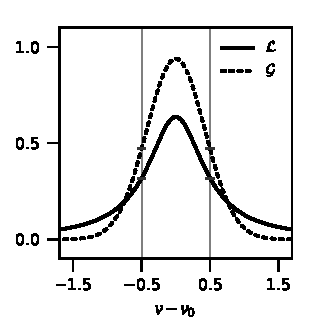
\includegraphics[width=\linewidth]{comparison}
\caption[Comparison of Lorentzian and Gaussian distributions]{\label{f.comparison}
Comparison of a Lorentzian ($\mathcal{L}$, solid line) and a Gaussian ($\mathcal{G}$, dotted line), both with $\mathrm{FWHM}=1$. The area under each curve is unity.}
\end{marginfigure}

\newthought{Consider an electronic transition in an atom between two energy levels, $E_m$ and $E_n$.} The natural frequency of this transition is $\nu_0 = |E_n-E_m|/h$. Light incident on the atom with frequency\sidenote{We are switching from angular frequency $\omega$ to frequency $\nu = \omega/2\pi$.} $\nu\neq\nu_0$ drives the electron at frequency $\nu$. An accelerating electron radiates, which damps the acceleration of the electron.  Classically, the transition in an atom is an electromagnetic oscillator with damping and driving terms, with cross-section\sidenote{For details, see the Box~\ref{b.line-emission}.}
\begin{equation}\label{e.semi-classical}
    \sigma = \left(\frac{\pi e^2}{m_e c}\right)
    \left\{\frac{\Gamma/4\pi}{(\nu_0-\nu)^2 + (\Gamma/4\pi)^2}\right\}.
\end{equation}
The actual value of the cross-section must be calculated using quantum mechanics. The overall shape of the cross-section is still in the form of equation~(\ref{e.semi-classical}) with opacity
\begin{equation}
    \rho\kappa_\nu = n_i \left(\frac{\pi e^2}{m_e c}\right) f_{mn}
        \left\{\frac{\Gamma/4\pi}{(\nu_0-\nu)^2 + (\Gamma/4\pi)^2}\right\}.
\end{equation}
In this equation, $f_{mn}$ is a number, called the \emph{oscillator strength}, that results from the calculation of the transition probability from state $m$ to state $n$, and $n_i$ is the density of atoms in state $m$.  The key point is that $f_{mn}$ depends only on the details of the transition: the energies, spins, and parities of the atomic states.  It does not depend on environmental parameters such as temperature and pressure.  As a result, $f_{mn}$ can be measured or computed once and then tabulated.


\begin{sidebar}[Treating line emission as a driven damped oscillator]
\label{b.line-emission}
NB. In this box, Gaussian CGS units are used for the electromagnetic field. To convert to MKS, make the following substitutions:
\begin{eqnarray*}
e &\to& \frac{1}{\sqrt{4\pi\varepsilon_0}}e\\
\bvec{E} &\to& \sqrt{4\pi\varepsilon_0}\bvec{E}\\
c &\to& (\mu_0\varepsilon_0)^{-1/2}.
\end{eqnarray*}

\newthought{Suppose we have a classical charged harmonic oscillator.}  The instantaneous power emitted by the oscillator is
\begin{equation}\label{e.larmor-power}
	 P(t) = \frac{2}{3}\frac{e^{2}}{c^{3}} |\dot{\vu}|^{2},
\end{equation}
and when averaged over a cycle is
\begin{equation}\label{e.oscillator-power}
	 \left\langle P(t) \right\rangle = \frac{e^{2}}{3c^{3}}x_{0}^{2} \omega^{4},
\end{equation}
since $\dot{\vu} = -\omega^{2}\bvec{x}_{0}\cos \omega t$. Since the oscillator is radiating, it is losing energy and is damped. Let us write the damping as $\bvec{F}_{\mathrm{rad}}\vdot \vu$; to find $\bvec{F}_{\mathrm{rad}}$, we integrate the power loss over a cycle,
\[  -\int_{t_{1}}^{t_{2}}\!\dif t\;\frac{2}{3}\frac{e^{2}}{c^{3}}\dot{\vu}\vdot\dot{\vu} 
	= -\left.\frac{2}{3}\frac{e^{2}}{c^{3}}\dot{\vu}\vdot\vu\right|_{t_{1}}^{t_{2}} 
	+ \frac{2}{3}\frac{e^{2}}{c^{3}} \int_{t_{1}}^{t_{2}}\!\dif t\;\ddot{\vu}\vdot\vu. 
\]
Since the motion is periodic, the first term vanishes and we can therefore identify 
\[ 
	\bvec{F}_{\mathrm{rad}} = \frac{2}{3}\frac{e^{2}}{c^{3}}\ddot{\vu} 
	= -m\left(\frac{2e^{2}\omega^{2}}{3c^{3}m}\right)\vu
\]
as the radiation damping term with the term in parenthesis being the damping constant $\gamma$. 
If there is an driving electric field on our oscillator, then its equation of motion becomes
\begin{equation}\label{e.eq-sho}
	m\ddot{\bvec{x}} = -m\omega_{0}^{2}\bvec{x} + e\bvec{E}e^{i\omega t} - m\gamma \dot{\bvec{x}}.
\end{equation}
Using a trial function $\bvec{x}\propto e^{i\omega t}$ gives
\[
	\bvec{x} = \frac{e}{m}\frac{E e^{i\omega t}}{(\omega_{0}^{2}-\omega^{2}) + i\omega\gamma}.
\]
Taking the second derivative w.r.t.\ time of $\bvec{x}$, substituting into eq.~(\ref{e.larmor-power}), and averaging over a cycle gives the power radiated by the oscillator,
\[
	\left\langle P(t)\right\rangle = \frac{e^{4}\omega^{4} E^{2}}{3 c^{2}m^{2}}
	\frac{1}{(\omega_{0}^{2}-\omega^{2})^{2} + \gamma^{2}\omega^{2}}.
\]
Dividing $\langle P(t)\rangle$ by the incident power per unit area, $cE^{2}/(8\pi)$, gives the cross-section:
\begin{equation}\label{e.classical-oscillator-cross-section}
	\sigma = \frac{8\pi}{3}\frac{e^{4}}{m^{2}c^{3}}
	\frac{\omega^{4}}{(\omega_{0}^{2}-\omega^{2})^{2} + \gamma^{2}\omega^{2}}.
\end{equation}
Now, for $\omega \approx \omega_{0}$, we can expand $(\omega_{0}^{2}-\omega^{2})^{2} \approx 4\omega_{0}^{2}(\omega_{0}-\omega)^{2}$; furthermore, we identify $2e^{2}\omega_{0}^{2}/(3c^{3}m) = \gamma$ and equation~(\ref{e.classical-oscillator-cross-section}) becomes
\begin{equation}\label{e.cross-section-lorentz}
	\sigma = \pi\left(\frac{e^{2}}{mc}\right)\frac{\gamma}{(\omega_{0}-\omega)^{2} + (\gamma/2)^{2}}.
\end{equation}
The line profile is Lorentzian, with a width $\gamma$. In terms of wavelength, the width is
\[ 
	\Delta \lambda = \left|\frac{\dif\lambda}{\dif\omega}\right|\gamma = \frac{2\pi c}{\omega^{2}}\gamma
	= \val{\sci{1.2}{-4}}{\textrm{\AA}}.
\]
This width is independent of the transition frequency (it is just the classical electron radius), and it is very, very small.  In a stellar atmosphere, the width is set by interactions and doppler broadening.

\newthought{To understand how impacts affect the line width}, suppose we model the oscillator as being started and stopped by impacts; in between impacts it just goes as $e^{i\omega_{0}t}$.  To get the spectrum, we take the Fourier transform,
\[
	F(\omega,t) = \int_{0}^{t}\!\dif t'\; \exp[i(\omega_{0}-\omega)t'],
\]
where $t$ is some time between impacts. Now if the impacts are distributed randomly and are uncorrelated, then the distribution of wait times follows a Poisson distribution,
\[ W(t)\,\dif t = e^{-t/\tau}\,\dif t/\tau, \]
where $\tau$ is the average time between collisions.  Using this to compute the energy spectrum, we obtain
\[ E(\omega) = \frac{1}{2\pi\tau}\int_{0}^{\infty}\!\dif t\; F(\omega,t)F^{*}(\omega,t)W(t) = \frac{1}{\pi\tau} 
	\frac{1}{(\omega_{0}-\omega)^{2} + (1/\tau)^{2}};
\]
the line profile is again Lorentzian, with a FWHM $2/\tau$.
\end{sidebar}

\newthought{There is an intrinsic width $\Gamma$ that is set by the finite lifetime of the energy levels;} in practice, however, this is not important.  In a stellar atmosphere, the width $\Gamma$ is set by collisions.  For example, when an electron passes close by our atom, the electric field shifts the energy levels of the atom\sidenote{This is an application of the \emph{Stark} effect that you learn about in quantum mechanics.}.  The greater the collision rate, the larger the width.
If we have two stars of the same photospheric temperature (so that both stars have the same lines), then a way to increase the collision rate is to increase the pressure. Recall, however, that in the stellar atmosphere $P = (g/\kappa)\tau$; as a result, stars with a higher surface gravity will have broader lines. The inset in Figure~\ref{f.compare_grav} illustrates the broadening of the Balmer H$\gamma$ line ($5\to 2$) in the spectrum of a main-sequence A1 star compared with that of a supergiant A1 star.

\begin{figure}[hp]
    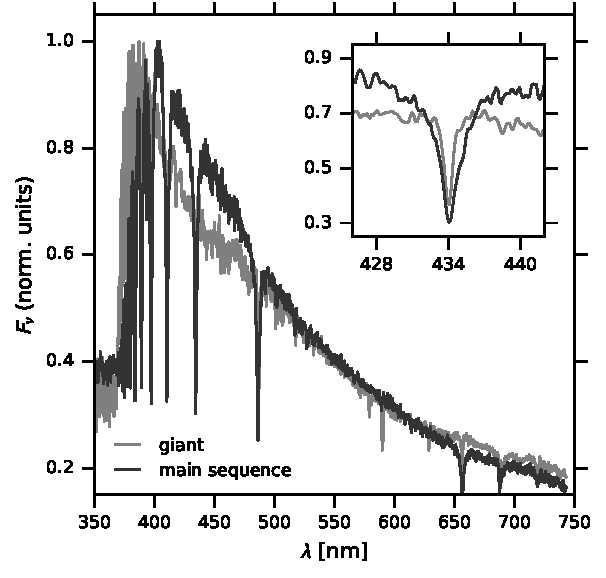
\includegraphics[width=\linewidth]{compare_grav}
    \caption[Spectra of two A1 stars]{\label{f.compare_grav}
    Spectra of two A1 stars, HD 16608 (a main sequence star) and SAO 12149 (a supergiant star).  Spectra are from \citet{Jacoby1984A-library-of-st}.
    }
\end{figure}

In addition to the width set by collisions, the line is also broadened by thermal motion: the atoms are in ceaseless motion; those headed towards us absorb at a blueshifted frequency, while those headed away from us absorb at a redshifted frequency.  Because the atomic velocities follow a Maxwell-Boltzmann distribution, the net effect is to make the core of the line (that is, near the center) assume a Gaussian profile.  Because a Gaussian falls off more quickly than a Lorentzian profile (see Fig.~\ref{f.comparison}), the wings of the line are still determined by the collision rate.

We might be inclined to treat the atoms as hard spheres, but this gives a large $\tau$, or equivalently a narrow line width. We are therefore led to consider longer-range interactions for setting the intrinsic line width. Table~\ref{t.perturbers} lists such interactions. For a given impact parameter, the interaction perturbs the energy levels; by integrating over a distribution of  impact parameters one gets the intrinsic damping. Of course, we should really use a quantum mechanical calculation.  We can scale our cross-section to the classical result (eq.~[\ref{e.cross-section-lorentz}]), however, by writing
\begin{equation}\label{e.cross-section}
	 \sigma_{\nu} = \left(\frac{\pi e^{2}}{m_{e}c}\right) f \phi_{\nu}, 
\end{equation}
where $\phi_{\nu}$ is the line profile (dimension $\sim \Hz^{-1}$) and $f$ is a dimensionless cross-section called the \newterm{oscillator strength}.

\begin{table}[htbp]
\caption{Interactions in stellar atmospheres}\label{t.perturbers}
\begin{tabular}{crcc}
\hline
perturbation & form & source & affects\\
\hline\hline
linear Stark & $C_{2} r^{-2}$ & $e^{-}$, $p$, ions & H (H$\alpha$, H$\beta$, \ldots)\\
quadratic Stark & $C_{4} r^{-4}$ & $e^{-}$ & non-hydrogenic ions\\
van der Waals & $C_{6}r^{-6}$ & atoms, H & most atomic lines, esp.\ in cool stars\\
\hline
\end{tabular}
\end{table}


\chapter{Hydrostatic Balance and Basic Stellar Properties}\label{ch.hydrostatic-balance}
% !TEX root = ../intro-stellar-physics.tex

\section{Virial Equilibrium}
\label{s.virial-equilibrium}

Let's consider a fluid at rest in a gravitational field. By \emph{at rest}, we simply mean that the fluid velocity is sufficiently small that we can neglect the inertia of the moving fluid in our equation for force balance.  By a \emph{fluid}, we mean that the pressure is isotropic\sidenote{Meaning the pressure is the same in all directions.} and directed perpendicular to a surface.  Let's now imagine a small fluid element, with thickness $\Delta r$ and cross-sectional area $\Delta A$, as depicted in Fig.~\ref{f.hydrostatic-equilibrium}.
\begin{marginfigure}
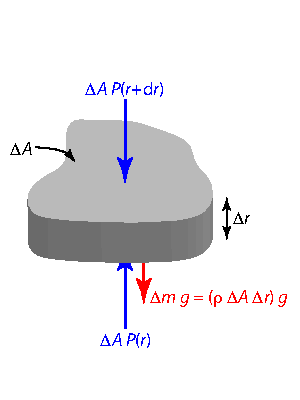
\includegraphics[width=\linewidth]{hydrostatic-equilibrium}
\caption[A fluid element in hydrostatic equilibrium]{A fluid element in hydrostatic equilibrium.
\label{f.hydrostatic-equilibrium}}
\end{marginfigure}

The force on the upper face is $\Delta A\times P(r+\Delta r)$; on the lower face, $\Delta A\times P(r)$.  Here $P(r)$ is the pressure.  For the element to be in hydrostatic equilibrium the forces must balance,
\[
        \Delta A \left[ -P(r+\Delta r) + P(r) - \Delta r \rho g(r)  \right] = 0;
\]
substituting for $g(r)$, dividing by $\Delta r$, taking the limit $\Delta r \to 0$ gives us the equation of hydrostatic equilibrium:
\begin{equation}\label{e.hydrostatic-equilibrium}
        \DD{P}{r} = -\rho \frac{Gm(r)}{r^{2}}.
\end{equation}
Here the mass enclosed within radius $r$ is
\begin{equation}\label{e.mass-continuity}
	m(r) = 4\pi \int_{0}^{r}\rho(r)r^{2}\,\dif r,
\end{equation}
with $\rho$ being the mass density.

With the assumption that $\rho = \textrm{constant}$, we showed that the central temperature and pressure depended on the total mass $M$, total radius $R$, and the gravitational constant $G$ as
\begin{eqnarray}
\label{e.Tc}
T_{c} &=& \frac{1}{2}\frac{GM}{R}\frac{\mu\mb}{\kB}\\
\label{e.Pc}
P_{c} &=& \frac{3}{8\pi}\frac{GM^{2}}{R^{4}}.
\end{eqnarray}
Here $\mu\mb$ is the average mass of a particle in the plasma. Our task now is to show that the scalings of $P$ and $T$ with $M$ and $R$ hold in general for an a star in mechanical equilibrium.

To show this, we are going to employ a form the \emph{virial theorem}.  Suppose we have a collection of $N$ particles, all moving about and exerting forces on one another.  If we let this system settle down into some kind of bound configuration, the virial theorem asserts that the kinetic energy $K$ is proportional to, and comparable in magnitude to, the potential energy $\Omega$; indeed if the potential between a pair of particles scales as $r^{-1}$, $r$ being the distance between the particles, then $K = -\Omega/2$.

Let us take the position and momentum of particle $i$ to be $\bvec{r}_{i} = (x_{i},y_{i},z_{i})$ and $\bvec{p}_{i}=(p_{x},p_{y},p_{z})$.  Then the total kinetic energy is
\begin{eqnarray}
\nonumber
	K &=& \frac{1}{2}\sum_{i=1}^{N}\bvec{p}_{i}\vdot\DDt{\bvec{r}_{i}}\\
		&=& \frac{1}{2}\left[\DDt{}\left(\sum_{i=1}^{N}\bvec{p}_{i}\vdot\bvec{r}_{i}\right) - \sum_{i=1}^{N}\bvec{r}_{i}\vdot\DDt{\bvec{p}_{i}}\right].
\label{e.expand-K}
\end{eqnarray}
The quantity $G = \sum_{i}\bvec{p}_{i}\vdot\bvec{r}_{i}$ is called the ``virial'' of the system.  By expressing the force $\bvec{F}_{i} = \dif\bvec{p}_{i}/\dif t$ on particle $i$ as the gradient of a potential $\Omega$, $\bvec{F}_{i} = -\grad_{i}\Omega$, we can rewrite eq.~(\ref{e.expand-K}) as
\begin{equation}\label{e.virial-deriv-1}
	2K = \DDt{G} + \sum_{i=1}^{N}\bvec{r}_{i}\vdot\grad_{i}\Omega.
\end{equation}
So far, we just shuffled and relabeled terms.  The crucial step comes in taking the time-average of the kinetic energy, which we'll denote by $\langle\;\rangle$:
\[	\langle f\,\rangle \equiv \lim_{\tau\to\infty} \frac{1}{\tau}\int_{0}^{\tau}f(t)\,\dif t. \]
Applying this to equation~(\ref{e.virial-deriv-1}) gives
\begin{eqnarray*}
	2\langle K\,\rangle &=&
		 \left\langle\DDt{G}\right\rangle 
		+ \left\langle\sum_{i=1}^{N}\bvec{r}_{i}\vdot\grad_{i}\Omega\right\rangle\\
	&=& \lim_{\tau\to\infty}\left[\int_{0}^{\tau}\,\DDt{G}\,\dif t\right] 
		+ \left\langle\sum_{i=1}^{N}\bvec{r}_{i}\vdot\grad_{i}\Omega\right\rangle\\
	&=& \underbrace{\lim_{\tau\to\infty}\left[\frac{G(\tau)-G(0)}{\tau}\right]}_{\mathrm{I}}
		+ \underbrace{\left\langle\sum_{i=1}^{N}\bvec{r}_{i}\vdot\grad_{i}\Omega\right\rangle}_{\mathrm{II}}
\end{eqnarray*}
Now, if the system is bound and in mechanical equilibrium, then the positions and momenta of all particles are finite: none of the particles can escape, and the system doesn't violently collapse so that momenta are diverging.  Hence both $G(\tau)$ and $G(0)$ are finite numbers, so as $\tau\to\infty$, term I vanishes.

As for term II, we can show that if the potential between pairs of particles depends on $1/r$, where $r$ is the distance between those particles, then term II is just $-\Omega$ (see Box~\ref{b.working-vectors}).  For now, I'll give a rough argument of why this is so:  in a spherically symmetric system, then the potential just depends on the distance $r$ from the origin; and since
\[
	r\dd{}{r} \left(\frac{1}{r}\right) = -\frac{1}{r},
\]
the last term is just $-\Omega$ and our equation is
\begin{equation}\label{e.virial-theorem}
2\langle K\,\rangle + \langle \Omega\rangle = 0.
\end{equation}
This is the virial theorem.

\begin{sidebar}[Working with vectors]
\label{b.working-vectors}
In this sidebar we'll show that the second term in equation~(\ref{e.virial-deriv-1}) is
\begin{equation}\label{e.term-2}
	\sum_{i=1}^{N}\bvec{r}_{i}\vdot\grad_{i}\Omega = -\Omega.
\end{equation}
First, we need an expression for $\Omega$. Suppose we pick a pair of particles, $i$ and $k$.  The potential between this pair is
\[
	-\frac{Gm_{i}m_{k}}{r_{ik}} = -\frac{Gm_{i}m_{k}}{\sqrt{(\bvec{r}_{i}-\bvec{r}_{k})^{2}}}.
\]
Our total potential consists of a sum over the potentials between all $N(N-1)/2$ unique pairs of particles,
\[
	\Omega = -\frac{Gm_{1}m_{2}}{\sqrt{(\bvec{r}_{1}-\bvec{r}_{2})^{2}}} - \ldots 
	-\frac{Gm_{i}m_{k}}{\sqrt{(\bvec{r}_{i}-\bvec{r}_{k})^{2}}} - \dots
\]
When we take the derivative in eq.~(\ref{e.term-2}), we apply $\bvec{r}_{i}\vdot\grad_{i}$ to each term in the potential.  For the term with the pair $i$, $k$, this will give
\begin{eqnarray*}
	\lefteqn{\sum_{i=1}^{N}\bvec{r}_{i}\vdot\grad_{i}\left(-\frac{Gm_{i}m_{k}}{\sqrt{(\bvec{r}_{i}-\bvec{r}_{k})^{2}}}\right)} \\
	&=& -Gm_{i}m_{k}\left[\bvec{r}_{i}\vdot\grad_{i}\left(\frac{1}{\sqrt{(\bvec{r}_{i}-\bvec{r}_{k})^{2}}}\right) + \bvec{r}_{k}\vdot\grad_{k}\left(\frac{1}{\sqrt{(\bvec{r}_{i}-\bvec{r}_{k})^{2}}}\right)\right].
\end{eqnarray*}
Since many of you aren't yet comfortable with vector expressions, we'll do this in detail for the $x$-component:
\begin{eqnarray*}
	\lefteqn{\left[\bvec{r}_{i}\vdot\grad_{i}\left(\frac{1}{\sqrt{(\bvec{r}_{i}-\bvec{r}_{k})^{2}}}\right) + \bvec{r}_{k}\vdot\grad_{k}\left(\frac{1}{\sqrt{(\bvec{r}_{i}-\bvec{r}_{k})^{2}}}\right)\right]_{x}}\\
	&=& x_{i}\dd{}{x_{i}}\left(\frac{1}{\sqrt{(\bvec{r}_{i}-\bvec{r}_{k})^{2}}}\right)
		+ x_{k}\dd{}{x_{k}}\left(\frac{1}{\sqrt{(\bvec{r}_{i}-\bvec{r}_{k})^{2}}}\right) \\
		&=& -\frac{x_{i}(x_{i}-x_{k})}{(\bvec{r}_{i}-\bvec{r}_{k})^{3/2}}
		+ \frac{x_{k}(x_{i}-x_{k})}{(\bvec{r}_{i}-\bvec{r}_{k})^{3/2}}\\
		&=& -\frac{(x_{i}-x_{k})^{2}}{(\bvec{r}_{i}-\bvec{r}_{k})^{3/2}}
\end{eqnarray*}
The $y$- and $z$-components are similar, giving
\begin{eqnarray*}
	\sum_{i=1}^{N}\bvec{r}_{i}\vdot\grad_{i}\left(-\frac{Gm_{i}m_{k}}{\sqrt{(\bvec{r}_{i}-\bvec{r}_{k})^{2}}}\right) &=& Gm_{i}m_{k}
	\frac{(\bvec{r}_{i}-\bvec{r}_{k})^{2}}{(\bvec{r}_{i}-\bvec{r}_{k})^{3/2}}\\
 &=& -\left(-\frac{Gm_{i}m_{k}}{\sqrt{(\bvec{r}_{i}-\bvec{r}_{k})^{2}}}\right).
\end{eqnarray*}
This can be done for every term in the sum, with the final result that
\[
	\sum_{i=1}^{N}\bvec{r}_{i}\vdot\grad_{i}\Omega = -\Omega.
\]
\end{sidebar}

For an ideal monatomic gas in thermal equilibrium, the mean kinetic energy of a particle in the gas is $K = (3/2)\kB T$, and we therefore may define an average temperature
\begin{equation}\label{e.Tbar}
	2 K = 3 N\kB \bar{T} = -\Omega.
\end{equation}
The total number of particles is $N=M/(\mu\mb)$, and so
\begin{equation}\label{e.mean-T}
\bar{T} = -\frac{1}{3}\Omega\frac{\mu\mb}{M\kB}.
\end{equation}
The total potential of the system depends on only three parameters: $G$, $M$, and $R$.  The only way to make a quantity having dimensions of energy is for
\[ \Omega \propto -\frac{GM^{2}}{R}, \]
and so
\[ \bar{T} \propto \frac{GM}{R}\frac{\mu\mb}{\kB}.  \]
By using the ideal gas law, $\bar{P} = \bar{\rho}(\kB/\mu\mb)\bar{T}$, we find
\[ \bar{P} \propto \frac{GM^{2}}{R^{4}}. \]
As a concrete example, let's compute $\Omega$ for a constant density sphere.
If we bring a small amount of mass $\dif m$ from infinity onto a sphere of mass $m$ and radius $r$, then the change in potential is \[ \dif\Omega = -\frac{Gm}{r}\,\dif m. \]
For a constant density, $r = R(m/M)^{1/3}$; upon substituting for $r$ we have
\[
	\Omega_{\textrm{const.\ den.}} = - \int_{0}^{M}\frac{GM^{1/3} m^{2/3}}{R}\,\dif m = -\frac{3}{5}\frac{GM^{2}}{R}.
\]
Using this in equation~(\ref{e.mean-T}) gives us the mean temperature, and hence pressure, for a constant density sphere,
\begin{eqnarray}\label{e.mean-T-rho}
\bar{T} &=& \frac{1}{5}\frac{GM}{R}\frac{\mu\mb}{\kB},\\
\label{e.mean-P}
\bar{P} &=& \frac{3}{20\pi}\frac{GM^{2}}{R^{4}}.
\end{eqnarray}
These are comparable to the central values, eqn.~(\ref{e.Tc}) and (\ref{e.Pc}).

\section{A closer look at hydrostatic equilibrium}
\label{s.closer-look}

Let's imagine what would happen if the star fell out of equilibrium.  Suppose we could turn off the pressure\marginnote{Maybe that's what the red goo in the \emph{Star Trek} movie was supposed to do?}.  The star would collapse; how long would this take?  Let's calculate the amount of time a particle would need to free-fall from the surface to the center.  We can get this from Kepler's law. Start with a circular orbit and deform it while keeping the center at one focus, as shown in Fig.~\ref{f.fall-to-center}.  

\begin{marginfigure}
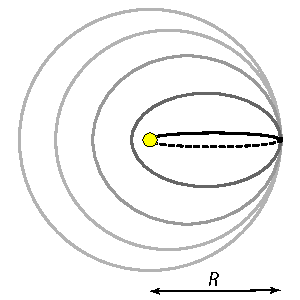
\includegraphics[width=\linewidth]{fall-to-center}
\caption[Fall to center]{\label{f.fall-to-center} Deformation of an orbit until it becomes a fall to the center, denoted by the yellow dot.}
\end{marginfigure}

The limit of these increasingly eccentric orbits is a fall into the center.  The time is one-half of an orbital period, and the semi-major axis in this limiting case is $a = R/2$:
\[
\tau_{\mathrm{ff}} = \frac{T}{2} = \frac{\pi}{\sqrt{GM}} \left(\frac{R}{2}\right)^{3/2}.
\]
Notice that we again have the combination $\sqrt{R^{3}/M}$.  Let's convert this into an expression involving the mean density $\bar{\rho}$:
\begin{equation}\label{e.tff}
\tau_{\mathrm{ff}} = \left(\frac{3}{32\pi}\right)^{1/2}\left(\frac{1}{G}\frac{4\pi R^{3}}{3M}\right)^{1/2} = \left(\frac{3}{32\pi}\right)^{1/2} \frac{1}{\sqrt{G\bar{\rho}}}.
\end{equation}
The time to collapse is proportional to $1/\sqrt{G\bar{\rho}}$ and depends on the average density of the star. We call $t_{\mathrm{dyn}} \equiv 1/\sqrt{G\bar{\rho}}$ the \emph{dynamical timescale} of the star.

Let's avoid a collapse by turning the pressure back on.  If part of the star is falling inward, the gas within the star will be compressed, the pressure will rise, and hydrostatic equilibrium will be restored.  How quickly can the star respond? A change is pressure is communicated to the rest of the star by sound waves, which travel at a speed (see Box~\ref{b.sound-speed})
\begin{equation}\label{e.speed-of-sound}
c_{s} = \left(\gamma\frac{P}{\rho}\right)^{1/2}
	= \left(\gamma\frac{\kB T}{\mu\mb}\right)^{1/2}.
\end{equation}
Here $\gamma$ is the adiabatic index: for an ideal monatomic gas, $\gamma = 5/3$.  How long would it take for a sound wave to go a distance $R$?  Using the expression for the average temperature of a constant density sphere from eq.~(\ref{e.mean-T-rho}), we find
\[
	\tau_{\mathrm{sc}} = \frac{R}{c_{s}} = R\left(\frac{3R}{GM}\right)^{1/2}
		= \left(\frac{3}{2\sqrt{\pi}}\right)\frac{1}{\sqrt{G\bar{\rho}}}.
\]
Both the sound-crossing time, $\tau_{\mathrm{sc}}$, and the free-fall time, $\tau_{\mathrm{ff}}$, are approximately equal to the dynamical timescale $1/\sqrt{G\bar{\rho}}$.  This is another way of looking at hydrostatic equilibrium: the star is able to remain in balance because the time for pressure disturbances to propagate, $\tau_{\mathrm{sc}}$, is comparable to the time for large-scale motions of the fluid, $\tau_{\mathrm{ff}}$.

\begin{sidebar}[The sound speed]
\label{b.sound-speed}
Suppose we have a long tube filled with gas at pressure $P(x,t) = P_{0}$, density $\rho(x,t) = \rho_{0}$, and velocity $u(x,t) = U_{0} = 0$. We then tap on one end of the tube; this causes a disturbance to propagate down the tube. Let's look at a small mass of fluid, located between $x$ and $x+\Delta x$; if the cross-sectional area of the tube is $A$, then the mass in this small volume is $\rho A\,\Delta x$.

As a result of the disturbance, the pressure in the tube becomes $P(x,t) = P_{0}+\sigma P_{1}(x,t)$. In this expression, $\sigma$ is a bookkeeping parameter that we'll eventually set to unity. We will expand our equations and keep only terms that are linear in $\sigma$. The fluid will also acquire a velocity $u(x,t) = \sigma u_{1}(x,t)$. This compresses or rarifies the gas: $\rho(x,t) = \rho_{0} + \sigma\rho_{1}(x,t)$.  Because the pressure in the tube is no longer uniform, our small mass will accelerate: 
\begin{eqnarray*}
	\rho A\,\Delta x \ddt{u} &=& A\,\Delta x\,(\rho_{0} + \sigma\rho_{1})\ddt{(0 + \sigma u_{1})}\\
	&\approx& \sigma\left[A\,\Delta x \rho_{0}\ddt{u_{1}}\right] + \mathcal{O}(\sigma^{2}).
\end{eqnarray*}
The corresponding force on our mass is
\[
	A \left[ P(x) - P(x+\Delta x) \right] \approx -\sigma A \left[P_{1}(x+\Delta x)-P_{1}(x)\right];
\]
equating this to the expression---to order $\sigma$---for the acceleration, taking the limit $\Delta x\to 0$, and canceling common factors gives
\begin{equation}\label{e.sound-speed-ut}
	\ddt{u_{1}} = -\frac{1}{\rho_{0}}\ddx{P_{1}}.
\end{equation}
Because of the non-uniform velocity, the volume and hence density of our little mass will also change:
\[
	\ddt{V} = A\left[u(x+\Delta x)-u(x)\right] 
		= \sigma A\,\Delta x\left[\frac{u_{1}(x+\Delta x)-u_{1}(x)}{\Delta x}\right]
\]
or
\begin{equation}\label{e.sound-speed-lnVt}
	\frac{1}{V}\ddt{V} = \sigma \ddx{u_{1}}.
\end{equation}
This change in volume is related to the change in pressure. We are interested in fluctuations that are sufficiently quick that no heat is transferred into or out of our mass. This is an adiabatic process, for which $PV^{\gamma} = \mathrm{const.}$. Here $\gamma$ is called the adiabatic index; for an ideal gas, this is the ratio of specific heats, $\gamma = C_{P}/C_{V}$.

As the pressure changes adiabatically from $P_{0}$ to $\sigma P_{1}$, the volume changes as
\[
	\frac{\dif V}{V} = \dif\ln V = -\frac{1}{\gamma}\dif\ln P.
\]
Hence
\begin{equation}\label{e.sound-speed-lnVt-2}
	\ddt{\ln V} = -\frac{1}{\gamma}\ddt{\ln (P_{0} + \sigma P_{1})} \approx 
		-\frac{\sigma}{\gamma P_{0}}\ddt{\ln P_{1}} = \sigma \ddx{u_{1}}.
\end{equation}
The last equality comes from equation (\ref{e.sound-speed-lnVt}).

We therefore have two equations for the perturbed velocity to order $\sigma$:
\begin{eqnarray*}
\ddt{u_{1}} &=& -\frac{1}{\rho_{0}} \ddx{P_{1}}\\
\ddx{u_{1}} &=& -\frac{1}{\gamma P_{0}} \ddt{P_{1}};
\end{eqnarray*}
differentiating the top equation with respect to $x$ and the bottom with respect to $t$, and equating the expressions for $\partial^{2}u_{1}/\partial t\partial x$ gives
\begin{equation}\label{e.sound-speed}
\frac{\partial^{2} P_{1}}{\partial t^{2}} = \left(\frac{\gamma P_{0}}{\rho_{0}}\right)
	\frac{\partial^{2} P_{1}}{\partial x^{2}}.
\end{equation}
This is the equation for a wave: the solutions are $P_{1}(x,t) = P_{1}(x\pm c_{s}t)$, where the sound speed is $c_{s} = \sqrt{\gamma P/\rho}$.
\end{sidebar}

For the sun, $\bar{\rho} = \val{1400}{\kilo\gram\usk\meter^{-3}} = \val{1.4}{\grampercc}$; this is just a bit denser than you.  The dynamical timescale for the sun is about one hour.

\section{Stellar Properties}
\label{s.stellar-properties}

We can infer a great deal from our simple virial scalings. Table~\ref{t.stellar-properties} provides masses and radii, in units of $\Msun$ and $\Rsun$, for stars from type B to type M.  If we assume that the stars have the same distribution of mass, so that the numerical coefficients in the expressions for $\rho_{c}$, $T_{c}$, and $P_{c}$ are the same, then for each star we may compute $\rho_{c}/\rho_{c,\odot} = (M/\Msun)(R/\Rsun)^{-3}$ and similarly for $T_{c}/T_{c,\odot}$ and $P_{c}/P_{c,\odot}$.

\begin{table}
\caption{\label{t.stellar-properties} Masses and radii for selected stellar types.}
\begin{tabular}{ld{4.2}d{3.2}d{1.2}d{1.2}d{1.2}d{2.3}}
 & \tabhead{B2} & \tabhead{B8} & \tabhead{F0} & \tabhead{G5} & \tabhead{M0} & \tabhead{M7}\\ 
\hline
$M/\Msun$ & 9.8 & 3.8 & 1.6 & 0.92 & 0.51 & 0.12\\
$R/\Rsun$ & 5.6 & 3.0 & 1.5 & 0.92 & 0.60 & 0.18\\
$L/\Lsun$ & 5800.0    & 180.0 & 6.5 & 0.79 & 0.08 & 0.003\\
$\rho_{c}/\rho_{c,\odot}$ & 0.06 & 0.14 & 0.47 & 1.18 & 2.36 & 20.58\\
\rowcolor{yellow}
$T_{c}/T_{c,\odot}$ & 1.75 & 1.27 & 1.07 & 1.00 & 0.85 & 0.67\\
$P_{c}/P_{c,\odot}$ & 0.10 & 0.18 & 0.51 & 1.18 & 2.01 & 13.72\\
\end{tabular}
\end{table}

Notice that $P_{c}$ and $\rho_{c}$ are larger for lower-mass stars. An even more surprising finding from this table is how little $T_{c}$ varies. This table spans nearly two decades in mass and six decades in luminosity, and yet $T_{c}$ varies by only a factor of three.  As we'll derive later, this is a consequence of the fusion reactions being extremely sensitive to temperature.

\section{Contraction to the main sequence}
\label{s.stellar-contraction}

Stars are born when a cold, dense\sidenote{Dense is a relative term; here we mean $\sim 100$ \emph{atoms} per cubic centimeter} cloud of gas and dust becomes unstable to gravitational collapse. The details of this process is a topic of current research; for our purposes, however, after a period of time a pre-main sequence star forms.  This object is in hydrostatic balance, but with a radius much larger than its main-sequence value.  As you know from the previous discussion, its central temperature will therefore be too low for fusion reactions to be important.  What happens to this object?

The pre-main sequence star is in hydrostatic balance, so it doesn't collapse. But the interior, and hence the surface, is warm, so it radiates energy.  The only source of energy is gravitational, so the pre-main sequence star \emph{must} contract.  How long would this take?  For our sun, the total energy is
\[
	E_{\odot} = K + \Omega = \Omega/2 \approx -\frac{G\Msun^{2}}{\Rsun};
\]
the time to radiate this energy away is
\begin{equation}\label{e.kelvin-helmholtz}
t_{\mathrm{KH}} = \frac{|E_{\odot}|}{\Lsun} \approx \frac{G\Msun^{2}}{\Rsun\Lsun} \approx \val{\sci{3}{7}}{\yr}.
\end{equation}
This timescale is called the \emph{Kelvin-Helmholtz timescale}.  Since $t_{\mathrm{KM}} \gg t_{\mathrm{dyn}}$ the star is, to an excellent approximation, in hydrostatic equilibrium throughout the whole contraction.

As the star contracts and $R$ decreases, the central density, pressure, and temperature increase.  When the central temperature becomes sufficiently hot, the heating from nuclear reactions rapidly increases and supplies enough energy to offset that radiated from the surface.  At this point the star is on the main-sequence, where it remains until the hydrogen fuel is exhausted from its core.



\chapter{Transport: The Mean Free Path}\label{ch.mean-free-path}
% !TEX root = ../intro-stellar-physics.tex

\newthought{Photons in a plasma, such as in the interior of the sun, transport energy.}  Were the sun transparent, these photons would immediately stream out, and the sun would release its stored energy in a fiery blast.  This doesn't happen: a photon can only travel a short distance before being scattered or absorbed. The net effect is that radiation generated in the core must travel a tortuous path, rather like a pinball, before reaching the surface and escaping.

How far does a photon---or any particle, for that matter---travel, on average, in the interior of the sun? Imagine a particle traveling with speed $v$.  Draw a cylinder, of length $\ell$ and cross-sectional area $\mathcal{A}$, around its future path, as shown in Fig.~\ref{f.MFP}. What the particle ``sees'' is that the cylinder is partly blocked by obstacles---other particles in its path. What is the probability of our particle making it through the cylinder unscathed?

\begin{marginfigure}
    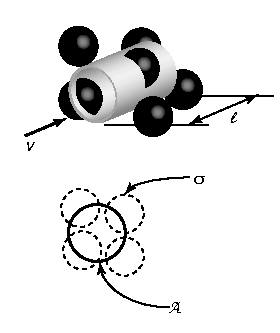
\includegraphics[width=\linewidth]{mean-free-path}
    \caption{\label{f.MFP} Schematic of a particle incident on a group of particles.}
\end{marginfigure}

The probability of the particle making it through is the ratio
\[
    \mathcal{P} = \frac{\textrm{total area covered by obstacles}}{\textrm{area of cylinder}}
\]
Denote the cross-sectional area of the other particles by $\sigma$.  If the density of obstacles is $n$, then the number of obstacles in the cylinder is $n\times(\mathcal{A}\ell)$, and therefore the fraction of the area blocked by the obstacles is
\begin{equation}
    \mathcal{P} = \frac{n\times(\mathcal{A}\ell)\times\sigma}{\mathcal{A}} = n\sigma\ell.
\label{e.prob-MFP}
\end{equation}
\marginnote{We are taking $\ell$ and $\mathcal{A}$ sufficiently small that we don't have to worry about particles overlapping.}
The particle will suffer a collision when $\mathcal{P}\to 1$, or when
\begin{equation}\label{e.MFP}
    \ell = \frac{1}{n\sigma}.
\end{equation}
We call $\ell$ the ``mean free path''.

\begin{exercisebox}[Mean free path for electron scattering]
    In the sun, free electrons scatter photons, and the cross-section is
    \[
    \sigma_{\mathrm{Th}} = \left(\frac{8\pi}{3}\right)\left(\frac{e^2}{m_e c^2}\right)^2 = \val{\sci{6.65}{-27}}{\meter^2}.
    \]
    What is the mean free path against this process for a photon?
\end{exercisebox}

\begin{exercisebox}[Mean free path of a hockey puck]\label{ex.MFP-2D}
    Suppose we have a flat surface on which pucks are sliding around, as shown in Fig.~\ref{f.MFP-2D} (Think of an air hockey table). The pucks bounce off the walls as they slide around.  Suppose there are $N$ pucks, each with a unit diameter, and the table is square with sides of length $L$.  Estimate the mean free path of a puck.
\end{exercisebox}

\begin{marginfigure}[-5\baselineskip]
    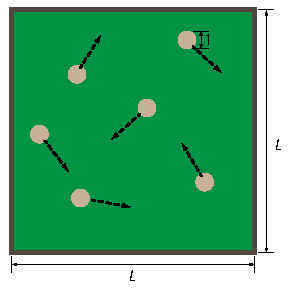
\includegraphics[width=\linewidth]{air-hockey-mfp}
    \caption[Mean free path of a hockey puck]{\label{f.MFP-2D}Schematic for Exercise~\ref{ex.MFP-2D}}
\end{marginfigure}

\chapter{A Closer Look at the Eddington Approximation}\label{ch.stellar-atmospheres}
% !TEX root = ../intro-stellar-physics.tex

We are now ready to investigate heat transport near the edge, where the optical depth $\tau_{\nu} \lesssim 1$ and photons begin to freely escape. We can no longer use the approximation of radiative diffusion, because conditions in the star are now changing over distances of a mean free path. Let's return to equation~(\ref{e.transfer-equation}) for radiative transport:
\[
	\DD{I_{\nu}}{s} = -\rho\left(\kapabs + \kapscat\right) I_{\nu} + \rho j_{\nu} + \rho\kapscat J_{\nu}.
\]
In general, this is difficult to solve: for some frequencies, the atmosphere will be nearly transparent, while for other frequencies it is quite opaque. Rather than develop the numerical machinery to solve the equation, we shall adopt a simple approximation that will allow us to obtain an approximate solution for the temperature of the stellar atmosphere.

\marginnote[\baselineskip]{\colorbox{yellow}{\textbf{Opacities are gray}}}We assume that the opacity is gray. That is, the opacity is independent of frequency. This is unphysical, but the solutions for temperature and pressure will have the correct overall behavior. Because the opacity is gray, we shall drop the ``$\nu$'' subscript in $\kappa$ and $\tau$.

\begin{exercisebox}[Gray emissivity?]
For matter with a gray opacity in thermal equilibrium, is the emissivity $j_{\nu}$ also gray?
\end{exercisebox}

We next define a coordinate system. Since we are in a thin layer near the edge of the star, we will adopt planar coordinates, with $z$ being the altitude above some point. We'll pick $z=0$ to be a point deep enough in the star that $I_{\nu}\approx B_{\nu}$. Then we define the optical depth as
\begin{equation}\label{e.optical-depth-planar}
	\tau = \int_{z}^{\infty} \rho\left(\kappa^{\mathrm{abs}}+\kappa^{\mathrm{sca}}\right)\,\dif z ;
\end{equation}
differentiating this expression gives
\[
	\DD{\tau}{z} = -\rho\left(\kappa^{\mathrm{abs}}+\kappa^{\mathrm{sca}}\right).
\]
Note the ``$-$'': in these coordinates, as $z$ gets larger, $\tau$ gets smaller.

We may rewrite the equation (\ref{e.hydrostatic-equilibrium-g}) of hydrostatic balance as
\begin{eqnarray}
	-\rho g = \DD{P}{z} &=& \DD{P}{\tau}\DD{\tau}{z} = -\rho\kappa,\nonumber\\
	\DD{P}{\tau} &=& \frac{g}{\kappa}.
\label{e.P-tau}
\end{eqnarray}
Since we are in a thin layer, we can take the gravitational acceleration $g$ as being approximately constant. By integrating hydrostatic equilibrium from where $\tau = 0, P = 0$ to where $\tau = 1$, we can get an approximate value of the photospheric pressure,
\[
	P_{\mathrm{ph}} = \int_{0}^{P_{\mathrm{ph}}}\,\dif P = \int_{0}^{1}\frac{g}{\kappa}\,\dif\tau \approx \frac{g}{\kappa}.
\]
\begin{quote}
\emph{The surface gravity sets the pressure at the \textbf{photosphere}, the location where the optical depth is of order unity and where photons can escape from the star.}
\end{quote}

\begin{exercisebox}[Photospheric pressure]
Suppose you observe a star that has a 10\% larger mass and 10\% larger radius than the Sun. All else being equal, how does the pressure at the photosphere of this star compare to that of the Sun?
\end{exercisebox}

\marginnote[\baselineskip]{\colorbox{yellow}{\textbf{Atmosphere is in steady-state LTE}}}
Next, we assume that the matter is in \newterm{local thermal equilibrium} (LTE). This means there is a well-defined temperature at each depth. Furthermore, the emissivity is related to the absorption opacity,
\[
	j_{\nu} = \kappa^{\mathrm{abs}}B_{\nu}.
\]
Note that this does \emph{not} imply anything about the radiation field. We can now take the radiative transfer equation (\ref{e.transfer-equation}) and substitue our definition of optical depth (eq.~[\ref{e.optical-depth-planar}]) to obtain
\begin{equation}\label{e.transfer-gray}
	\mu\DD{I_{\nu}}{\tau} = I_{\nu} - S_{\nu}.
\end{equation}
Here
\[
	S_{\nu} = \frac{j_{\nu} + \kappa^{\mathrm{sca}} J_{\nu}}{\kappa}
	= \frac{\kappa^{\mathrm{abs}} B_{\nu} + \kappa^{\mathrm{sca}} J_{\nu}}{\kappa}.
\]
If, in addition, the matter is in steady-state, then the rate at which energy is absorbed from the radiation field, $\int\kappa^{\mathrm{abs}}I_{\nu}\,\dif\nu\,\dif\Omega$, must equal the rate at which energy is emitted, $\int j_{\nu}\,\dif\nu\,\dif\Omega$. Since we are in LTE,
\[
	\int \left(j_{\nu} - \kappa^{\mathrm{abs}}I_{\nu}\right)\,\dif\nu\,\dif\Omega
	= 4\pi\kappa^{\mathrm{abs}}\int\left(B_{\nu} - J_{\nu}\right)\,\dif\nu = 0.
\]
Since $J = \int J_{\nu}\,\dif\nu = \int B_{\nu}\,\dif\nu = B$, it follows that $S = \int S_{\nu}\,\dif\nu = B$ as well:
\begin{quote}
\emph{For a gray atmosphere in steady-state, local thermal equilibrium, the integrated source function and mean intensity equal the Planck value:}
\[ S(\tau) = J(\tau) = B(\tau), \]
\end{quote}
Note that this does \emph{not} imply that $I_{\nu}=B_{\nu}$ or $J_{\nu}=B_{\nu}$.

We still have the problem that eq.~(\ref{e.transfer-gray}) includes both the derivative and integral of $I_{\nu}$. To get around this, we are going to expand $I_{\nu}$ in Legendre polynomials,
\[
	I_{\nu}(\tau,\mu) = I_{\nu,0}(\tau)\Pl{0}(\mu) + I_{\nu,1}(\tau)\Pl{1}(\mu) + I_{\nu,2}(\tau)\Pl{2}(\mu) + \ldots
\]
and then only include the first two terms, $\Pl{0}(\mu) = 1, \Pl{1} = \mu$. Thus, $I_{\nu}$ is \emph{linear} in $\mu$: $I_{\nu} = I_{\nu,0}(\tau) + I_{\nu,1}(\tau)\mu$. 
\marginnote{\colorbox{yellow}{\textbf{Intensity is linear in $\mu$}}}

In terms of this expansion, the angle-averaged specific intensity is
\[
	J_{\nu}(\tau) = \frac{1}{4\pi}\int I_{\nu}\,\dif\mu\,\dif\phi = I_{\nu,0}(\tau),
\]
and hence the specific energy density is $U_{\nu} = 4\pi/c\cdot J_{\nu} = 4\pi/c\cdot I_{\nu,0}$. The specific flux is
\[
	F_{\nu}(\tau) = \int \mu I_{\nu}\,\dif\mu\,\dif\phi = \frac{4\pi}{3} I_{\nu,1}(\tau).
\]
We can therefore write the intensity as
\begin{equation}
\label{e.intensity-expanded}
I_{\nu}(\tau) = J_{\nu}(\tau) + \frac{3\mu}{4\pi} F_{\nu}(\tau) = \frac{c}{4\pi}U_{\nu}(\tau) + \frac{3\mu}{4\pi} F_{\nu}(\tau).
\end{equation}

\begin{sidebar}[Expansion in Legendre polynomials]
\label{sb.intensity-decomposition}
You may recall from electrostatics that we can decompose the field from a set of charges into a sum of moments: dipole, quadrupole, and so on. The basis functions for this are the Legendre polynomials $\Pl{n}(\cos\theta)$, defined by the expansion
\[
	\frac{1}{\sqrt{1 - 2\mu z + z^{2}}} \equiv \sum_{n=0}^{\infty}\Pl{n}(\mu)z^{n},
\]
for $-1<\mu<1,\;|z| < 1$. The first four polynomials are
\begin{eqnarray*}
	\Pl{0}(\mu) = 1 &\quad& \Pl{2}(\mu) = \frac{1}{2}(3\mu^{2}-1)\\
	\Pl{1}(\mu) = \mu &\quad& \Pl{3}(\mu) = \frac{1}{2}(5\mu^{3}-3\mu),
\end{eqnarray*}
and the first eight Legendre polynomials are plotted below.

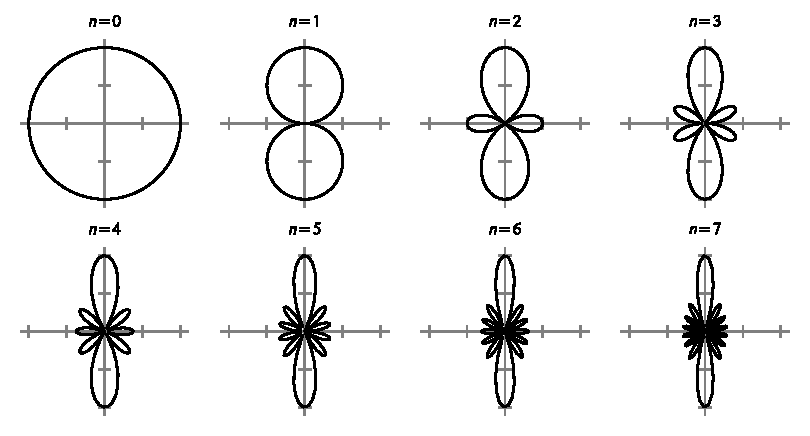
\includegraphics{legendre}

\noindent As $n$ increases, the angular scale of variations becomes finer.

The Legendre polynomials are \emph{orthogonal} in the following sense:
\begin{equation}\label{e.orthogonal}
\int_{-1}^{1}\Pl{n}(\mu)\Pl{m}(\mu)\dif \mu = \left\{
\begin{array}{lr}
	0 &  m\neq n\\
	\frac{2}{2n+1} & m=n
\end{array}\right..
\end{equation}
As a result of this orthogonality, we can decompose the radiative intensity into multipoles:
\begin{equation}\label{e.decomposition}
	I = \sum_{n=0}^{\infty} I_{n} \Pl{n}(\mu).
\end{equation}

\begin{exercisebox}[Odd-even powers of $\mu$]
\label{e.symmetry-powers-mu}
Use eq.~(\ref{e.orthogonal}) to show that $(4\pi)^{-1}\int I\,\dif\Omega = I_{0}$ and $\int \mu I\,\dif\Omega = (4\pi/3)I_{1}$, for $I = I_{0} + I_{1}\mu$.
\end{exercisebox}

\end{sidebar}

Insert the expansion (\ref{e.intensity-expanded}) into the radiative transfer equation (\ref{e.transfer-gray}) and integrate over all angles and frequencies. Since $\tau$ is gray, we can pull the derivative out from the integral,
\begin{eqnarray*}
	\DD{}{\tau}\int \mu I_{\nu}\,\dif\nu\,\dif\Omega &=& \int I_{\nu}\,\dif\nu\,\dif\Omega - \frac{\kappa^{\mathrm{abs}}}{\kappa}\int B_{\nu}\,\dif\nu\,\dif\Omega - \frac{\kappa^{\mathrm{sca}}}{\kappa} \int J_{\nu}\,\dif\nu\,\dif\Omega\\
	\DD{}{\tau}\int F_{\nu}\,\dif\nu &=& \frac{4\pi}{\kappa}\left[
		(\kappa^{\mathrm{abs}}+\kappa^{\mathrm{sca}})\int J_{\nu}\,\dif\nu
		- \kappa^{\mathrm{abs}}\int B_{\nu}\,\dif\nu
		- \kappa^{\mathrm{sca}}\int J_{\nu}\,\dif\nu\right]\\
	\DD{F}{\tau} &=& 4\pi\frac{\kappa^{\mathrm{abs}}}{\kappa}\int\left(J_{\nu}-B_{\nu}\right) = 0.
\end{eqnarray*}
Here we used $\kappa = \kappa^{\mathrm{abs}}+\kappa^{\mathrm{sca}}$ to simplify the right-hand side.

\begin{quote}
\emph{For a steady-state gray atmosphere in local thermal equilibrium, the total flux $F = \int F_{\nu}\,\dif\nu$ is constant.}
\end{quote}
The radiative energy is just passing through. Since the flux at $\tau=0$, outside the star, is $F = \sigmaSB\,\Teff^{4}$, we can substitute that value in our expression for the intensity,
\begin{equation}
\label{e.Inu-expansion}
	I(\mu,\tau) = \frac{c}{4\pi} U(\tau) + \frac{3\mu}{4\pi}\sigmaSB\Teff^{4}.
\end{equation}
To solve for $U_{\nu}(\tau)$, multiply eq.~(\ref{e.transfer-gray}) by $\mu$ and integrate over all angles and frequencies:
\begin{eqnarray}
	\DD{}{\tau}\int\mu^{2}I\,\dif\Omega\,\dif\nu &=& \int\mu I\,\dif\Omega\,\dif\nu
		- \int \mu S\,\dif\Omega\,\dif\nu\nonumber\\
	\frac{c}{4\pi}\DD{}{\tau} \mu^{2}U\,\dif\Omega 
		+ \frac{3}{4\pi}\sigmaSB\Teff^{4}\int\mu^{3}\,\dif\Omega &=& F - \int \mu S\,\dif\Omega\nonumber\\
	\frac{c}{3}\DD{U}{\tau} &=& \sigmaSB\Teff^{4}
\label{e.ODE-U}
\end{eqnarray}
In going from the first to the second line we have used eq.~(\ref{e.Inu-expansion}). In going from the second to the third line, the integrals of $\mu^{3}$ and $\mu S$ vanish because $S$ is independent of angle and $\int_{-1}^{1} \mu\,\dif\mu = \int_{-1}^{1}\mu^{3}\,\dif\mu = 0$. 

Equation~(\ref{e.ODE-U}) is a first-order ODE, which upon integration yields
\begin{equation}\label{e.energy-density-Eddington}
	U(\tau) = \frac{3}{c}F(\tau + \tau_{0}),
\end{equation}
where $\tau_{0}$ is an integration constant. Our intensity is thus
\[
	I(\mu,\tau) = \frac{3}{4\pi}\sigmaSB\Teff^{4}\left(\tau + \tau_{0} + \mu\right).
\]
To fix the integration constant $\tau_{0}$, let's go to where $\tau=0$. Here all of the radiation must be outward-bound. Hence if we integrate $\mu I(\mu,\tau=0)$ over $0\le\mu\le 1$, we should recover the flux:
\[
	\sigmaSB\Teff^{4} = \int_{0}^{2\pi}\int_{0}^{1} \mu I(\mu,\tau=0)\,\dif\mu\,\dif\phi
	= \frac{3}{4}\sigmaSB\Teff^{4}\left(\tau_{0} + \frac{2}{3}\right),
\]
which fixes $\tau_{0} = 2/3$.

To finish this, we note that $J = B$ since we are in steady-state local thermal equilibrium. The radiative energy density is thus $U = (4\pi/c) J = (4\pi/c)B = 4\sigmaSB/c T^{4}$. Substituting this into eq.~(\ref{e.energy-density-Eddington}) then yields
\begin{equation}\label{e.T-tau}
T^{4} = \frac{3}{4}\Teff^{4}\left(\tau + \frac{2}{3}\right).
\end{equation}
This equation, along with eq.~(\ref{e.P-tau}), determines the structure of the stellar atmosphere.

\begin{sidebar}[Decomposition of intensity into moments]
\label{sb.intensity-moments}
It is often useful to describe the intensity in terms of \newterm{moments}. A moment is simply an angle-weighted average of the radiative intensity. For example, to take the zeroth-order moment, we multiply $I_{\nu}$ by $\mu^{0}=1$, integrate over all angles, and divide by $4\pi$. This is just the average intensity $J_{\nu} = (4\pi)^{-1}\int I_{\nu}\,\dif\Omega$. To take the first-order moment, we use a weight $\mu^{1}$:
\[
	H_{\nu} = \frac{1}{4\pi}\int_{0}^{2\pi}\int_{-1}^{1}\mu I_{\nu}\,\dif\mu\,\dif\phi.
\]
To take the second-order moment, we use a weight $\mu^{2}$:
\[
	K_{\nu} = \frac{1}{4\pi}\int_{0}^{2\pi}\int_{-1}^{1}\mu^{2} I_{\nu}\,\dif\mu\,\dif\phi.
\]
The first three moments have physically interpretable meanings: the specific radiative energy density, flux, and pressure are $U_{\nu} = (4\pi/c)J_{\nu}$, $F_{\nu} = 4\pi H_{\nu}$, and $P_{\nu} = (4\pi/c) K_{\nu}$, respectively.



Notice that we can write the weighting factors in terms of Legendre polynomials:
\begin{eqnarray*}
	J &=& \frac{1}{4\pi}\int\,\dif\phi\dif\mu\,{\color{red}\mu^{0}}\,I 
		= \frac{1}{2}\int_{-1}^{1}\dif\mu\sum_{n=0}^{\infty} \,{\color{red}\Pl{0}} I_{n} \\
	H &=& \frac{1}{4\pi}\int\,\dif\phi\dif\mu\,{\color{red}\mu^{1}}\,I 
		= \frac{1}{2}\int_{-1}^{1}\dif\mu\sum_{n=0}^{\infty} \,{\color{red}\Pl{1}} I_{n} \\
	K &=& \frac{1}{4\pi}\int\,\dif\phi\dif\mu\,{\color{red}\mu^{2}}\,I 
		= \frac{1}{2}\int_{-1}^{1}\dif\mu\sum_{n=0}^{\infty} \,{\color{red} \frac{1}{3}(2\Pl{2}+\Pl{0})} I_{n}
\end{eqnarray*}
Now we can use the orthogonality relation (eq.~[\ref{e.orthogonal}]) to compute the integrals:
\begin{eqnarray*}
	J &=& I_{0} \\
	H &=& \frac{1}{3}I_{1} \\
	K &=& \frac{1}{3}\left(\frac{2}{5}I_{2} + I_{0}\right)
		= \frac{1}{3}\left(\frac{2}{5}I_{2} + J\right)
\end{eqnarray*}
Applying the Eddington approximation, i.e., setting $K = J/3$, means that we must set $I_{2} = 0$. Once we do this, we can solve for $J$, $H$, and $K=J/3$ as functions of optical depth $\tau$. This gives us a description of the radiative intensity in terms of $J(\tau)$ and $H$,
\[
	I(\tau,\mu) = J(\tau) + 3H \Pl{1}(\mu) + \cdots \approx J(\tau) + 3H\cos\theta,
\]
which neglects the higher order terms $I_{n}\Pl{n},\forall n > 2$.
\end{sidebar}


\newcommand*{\DDtt}[1]{\frac{\dif^{2} #1}{\dif t^{2}}}
\newcommand*{\wt}{\omega t}
\newcommand*{\wot}{\omega_{0} t}
\newcommand*{\wmt}{\omega_{m} t}
\newcommand*{\womw}{(\omega_{0}^{2}-\omega^{2})}
\newcommand*{\gw}{\Gamma^{2}\omega^{2}}

\nocite{Mihalas1978Stellar-Atmosph,LeBlanc2010An-Introduction,Carroll2006An-Introduction}

\section{Atomic Lines}

Let's begin with a simple system: a mass $m$ attached to a spring with force constant $k$ as shown in Fig.~\ref{f.simple-spring}.

\begin{marginfigure}[-8\baselineskip]
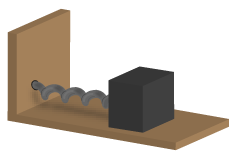
\includegraphics[width=\linewidth]{simple-spring}
\caption[A simple harmonic oscillator]{A simple harmonic oscillator: a mass $m$ on a frictionless surface attached to a  spring with force $F = -kx$.
\label{f.simple-spring}}
\end{marginfigure}

\subsection{With no driving force}

If we put the origin of our coordinate system where the mass is at rest with the spring relaxed, then the equation of motion of the mass is
\begin{equation}\label{e.SHO-basic}
	\DDtt{x} + \frac{k}{m} x = 0.
\end{equation}
You have solved this before: the most general solution is
\begin{equation}\label{e.SHO-general-solution}
	x(t) = x_{0}\cos(\wot) + \frac{v_{0}}{\omega_{0}}\sin(\wot)
\end{equation}
with $\omega_{0}^{2} = k/m$ and with $x_{0}$ and $v_{0}$ being the initial position and velocity of the mass.

\subsection{With driving at frequency $\omega \neq \omega_{0}$}

Now let's push on our mass with an oscillating force, $F\cos(\omega t)$ with $\omega\neq\omega_{0}$. A real world example would be holding a vibrating tuning fork near another fork tuned to a different frequency.  The equation of motion is now
\begin{equation}\label{e.SHO-driven}
	\DDtt{x} + \omega_{0}^{2}x = \frac{F}{m}\cos(\wt).
\end{equation}
You can verify by substitution that a general solution is
\[
	x(t) = \frac{F/m}{(\omega_{0}^{2}-\omega^{2})}\cos(\wt) + A\cos(\wot)+B\sin(\wot).
\]
Let's start with our harmonic oscillator at rest ($v_{0} = \left.\dif x/\dif t\right|_{t=0} = 0$) and at $\left. x\right|_{t=0} = 0$.  With these conditions, we can determine the constants $A$ and $B$; the solution is
\[
	x(t) = \frac{F/m}{(\omega_{0}^{2}-\omega^{2})}\left[\cos(\wt)-\cos(\wot)\right].
\]
Let's recast this by defining $\Delta = \omega_{0} - \omega$ and $\omega_{m} = (\omega_{0}+\omega)/2$.  Then
\begin{eqnarray*}
  \omega_{0}^{2}-\omega^{2} &=& (\omega_{0}-\omega)(\omega_{0}+\omega) = 2\Delta\omega_{m},\\
  \cos(\wot) &=& \cos\left(\wmt+\Delta t/2\right) = \cos(\wmt)\cos(\Delta t/2) - \sin(\wmt)\sin(\Delta t/2),\\
  \cos(\wt) &=& \cos\left(\wmt-\Delta t/2\right) = \cos(\wmt)\cos(\Delta t/2) + \sin(\wmt)\sin(\Delta t/2);
\end{eqnarray*}
and we write the solution as
\begin{equation}\label{e.beats}
	x(t) = \left[\frac{F/m}{\Delta\omega_{m}}\sin(\Delta t/2)\right]\sin(\wmt).
\end{equation}
This illustrates the phenomena of beats: the oscillation consists of a carrier signal at frequency $\omega_{m}$ with the amplitude modulated at the slower frequency $\Delta /2$.  Notice that the amplitude increases as $\Delta \to0$, i.e., $\omega\to\omega_{0}$.

\subsection{With both driving and damping}

Now let's make our model even more realistic by adding some damping.  We add a frictional force that is proportional to velocity, $F_{\mathrm{friction}} = -m\Gamma \dif x/\dif t$. Our complete equation of motion is then
\begin{equation}
	\DDtt{x} + \Gamma \DDt{x} + \omega_{0}^{2}x = \frac{F}{m}\cos(\omega t).
\end{equation}
The solution to this is straightforward to find, although the algebra is tedious (trust me on this). The general solution for initial conditions $\left.x\right|_{t=0} = x_{0}$ and $\left.\dif x/\dif t\right|_{t=0} = v_{0}$ is
\begin{eqnarray}
\label{e.general-solution-ddo}
\lefteqn{x(t) = \frac{F\womw/m}{\womw^{2}+\gw}\cos(\omega t)} && \\
	&+& \frac{\Gamma\omega F/m}{\womw^{2}+\gw}\sin(\omega t)\nonumber \\
	&+& \left[x_{0}-\frac{F\womw/m}{\womw^{2}+\gw}\right]{\color{red}e^{-\Gamma t/2}} \cos(\omega_{\Gamma}t) \nonumber\\
	&+& \left[\frac{v_{0}}{\omega_{\Gamma}}-\frac{\Gamma\omega F/m}{\womw^{2}+\gw}
	\,\frac{\omega}{\omega_{\Gamma}}\right]{\color{red}e^{-\Gamma t/2}} \sin(\omega_{\Gamma}t), 
	\nonumber
\end{eqnarray}
with
\[ 
    \omega_{\Gamma} = 
        \omega_{0}\left(1-\frac{\Gamma^{2}}{4\omega_{0}^{2}}\right)^{1/2}.
\]
Let's simplify this to the most relevant case.  First, the last two terms decay as {\color{red}$e^{-\Gamma t/2}$}: these are transients set by the initial conditions. After a time $2/\Gamma$ there will only be the first two terms, which oscillate at frequency $\omega$. 

We can simplify these first two terms even further: write
\[ \cos(\wt) = \frac{e^{i\wt}+e^{-i\wt}}{2},\quad \sin(\wt) 
    = \frac{e^{i\wt}-e^{-i\wt}}{2i}; \]
and combine terms to find
\begin{eqnarray}
    x(t) &=& \frac{F}{2m}\left[\frac{1}{\left(\omega_0^2-\omega^2\right) + i\Gamma\omega}\right]e^{i\wt} + \frac{F}{2m}\left[\frac{1}{\left(\omega_0^2-\omega^2\right) - i\Gamma\omega}\right]e^{-i\wt} \nonumber\\
    &=& \Re\left\{\frac{F}{m}\left[\frac{1}{\left(\omega_0^2-\omega^2\right) + i\Gamma\omega}\right]e^{i\wt}\right\}\label{e.oscillator-expression}
\end{eqnarray}
We use the symbol ``$\Re$'' to denote taking the real part of a complex quantity.  

From Eq.~(\ref{e.oscillator-expression}), we see that the oscillator can be described as the real part of a complex quantity $Ae^{i\wt}$, with
\[
    A = \frac{F}{m}\left[\frac{1}{\left(\omega_0^2-\omega^2\right) + i\Gamma\omega}\right].
\]
For $\omega \approx \omega_0$, we write $(\omega_0^2-\omega^2)\approx 2\omega_0(\omega_0-\omega)$ and take the square of the amplitude to find,
\begin{eqnarray}
    \left|A\right|^2 &=& \left(\frac{F}{2m\omega_0}\right)^2
        \frac{1}{(\omega_0-\omega)^2 + (\Gamma/2)^2}\nonumber\\
    &=& \frac{\pi}{2\Gamma}\left(\frac{F}{m\omega_0}\right)^2
        \left\{\frac{1}{\pi}\frac{\Gamma/2}{(\omega_0-\omega)^2 + (\Gamma/2)^2}\right\}
\end{eqnarray}
We rewrote the amplitude in the second line so that the term in $\{\cdot\}$ is normalized. The function
\[
    \mathcal{L}(\omega;\Gamma) = \frac{1}{\pi} 
        \frac{\Gamma/2}{(\omega_0-\omega)^2 + (\Gamma/2)^2}
\]
is known as a Lorentzian.  In contrast to a Gaussian, a Lorentzian is characterized by broad ``wings'' (Fig.~\ref{f.comparison}) as it goes to zero away from the central frequency $\omega_{0}$.
\begin{marginfigure}[-4\baselineskip]
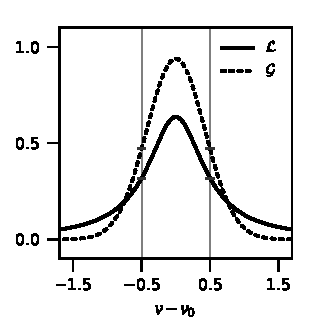
\includegraphics[width=\linewidth]{comparison}
\caption[Comparison of Lorentzian and Gaussian distributions]{\label{f.comparison}
Comparison of a Lorentzian ($\mathcal{L}$, solid line) and a Gaussian ($\mathcal{G}$, dotted line), both with $\mathrm{FWHM}=1$. The area under each curve is unity.}
\end{marginfigure}

\section{Atomic Lines}
You may be thinking, ``What does this have to do with atomic lines?'' Consider an electronic transition in an atom between two energy levels, $E_m$ and $E_n$. The natural frequency of this transition is $\nu_0 = |E_n-E_m|/h$. Light incident on the atom with frequency\sidenote{We are switching from angular frequency $\omega$ to frequency $\nu = \omega/2\pi$.} $\nu\neq\nu_0$ drives the electron at frequency $\nu$. An accelerating electron radiates, which damps the acceleration of the electron.  Classically, the transition in an atom is an electromagnetic oscillator with damping and driving terms, with cross-section\sidenote{For details, see the Box~\ref{b.line-emission}.}
\begin{equation}\label{e.semi-classical}
    \sigma = \left(\frac{\pi e^2}{m_e c}\right)
    \left\{\frac{\Gamma/4\pi}{(\nu_0-\nu)^2 + (\Gamma/4\pi)^2}\right\}.
\end{equation}
The actual value of the cross-section must be calculated using quantum mechanics. The overall shape of the cross-section is still in the form of equation~(\ref{e.semi-classical}) with opacity
\begin{equation}
    \rho\kappa_\nu = n_i \left(\frac{\pi e^2}{m_e c}\right) f_{mn}
        \left\{\frac{\Gamma/4\pi}{(\nu_0-\nu)^2 + (\Gamma/4\pi)^2}\right\}.
\end{equation}
In this equation, $f_{mn}$ is a number, called the \emph{oscillator strength}, that results from the calculation of the transition probability from state $m$ to state $n$, and $n_i$ is the density of atoms in state $m$.  The key point is that $f_{mn}$ depends only on the details of the transition: the energies, spins, and parities of the atomic states.  It does not depend on environmental parameters such as temperature and pressure.  As a result, $f_{mn}$ can be measured or computed once and then tabulated.


\begin{sidebar}[Treating line emission as a driven damped oscillator]
\label{b.line-emission}
NB. In this box, Gaussian CGS units are used for the electromagnetic field. To convert to MKS, make the following substitutions:
\begin{eqnarray*}
e &\to& \frac{1}{\sqrt{4\pi\varepsilon_0}}e\\
\bvec{E} &\to& \sqrt{4\pi\varepsilon_0}\bvec{E}\\
c &\to& (\mu_0\varepsilon_0)^{-1/2}.
\end{eqnarray*}

\newthought{Suppose we have a classical charged harmonic oscillator.}  The instantaneous power emitted by the oscillator is
\begin{equation}\label{e.larmor-power}
	 P(t) = \frac{2}{3}\frac{e^{2}}{c^{3}} |\dot{\vu}|^{2},
\end{equation}
and when averaged over a cycle is
\begin{equation}\label{e.oscillator-power}
	 \left\langle P(t) \right\rangle = \frac{e^{2}}{3c^{3}}x_{0}^{2} \omega^{4},
\end{equation}
since $\dot{\vu} = -\omega^{2}\bvec{x}_{0}\cos \omega t$. Since the oscillator is radiating, it is losing energy and is damped. Let us write the damping as $\bvec{F}_{\mathrm{rad}}\vdot \vu$; to find $\bvec{F}_{\mathrm{rad}}$, we integrate the power loss over a cycle,
\[  -\int_{t_{1}}^{t_{2}}\!\dif t\;\frac{2}{3}\frac{e^{2}}{c^{3}}\dot{\vu}\vdot\dot{\vu} 
	= -\left.\frac{2}{3}\frac{e^{2}}{c^{3}}\dot{\vu}\vdot\vu\right|_{t_{1}}^{t_{2}} 
	+ \frac{2}{3}\frac{e^{2}}{c^{3}} \int_{t_{1}}^{t_{2}}\!\dif t\;\ddot{\vu}\vdot\vu. 
\]
Since the motion is periodic, the first term vanishes and we can therefore identify 
\[ 
	\bvec{F}_{\mathrm{rad}} = \frac{2}{3}\frac{e^{2}}{c^{3}}\ddot{\vu} 
	= -m\left(\frac{2e^{2}\omega^{2}}{3c^{3}m}\right)\vu
\]
as the radiation damping term with the term in parenthesis being the damping constant $\gamma$. 
If there is an driving electric field on our oscillator, then its equation of motion becomes
\begin{equation}\label{e.eq-sho}
	m\ddot{\bvec{x}} = -m\omega_{0}^{2}\bvec{x} + e\bvec{E}e^{i\omega t} - m\gamma \dot{\bvec{x}}.
\end{equation}
Using a trial function $\bvec{x}\propto e^{i\omega t}$ gives
\[
	\bvec{x} = \frac{e}{m}\frac{E e^{i\omega t}}{(\omega_{0}^{2}-\omega^{2}) + i\omega\gamma}.
\]
Taking the second derivative w.r.t.\ time of $\bvec{x}$, substituting into eq.~(\ref{e.larmor-power}), and averaging over a cycle gives the power radiated by the oscillator,
\[
	\left\langle P(t)\right\rangle = \frac{e^{4}\omega^{4} E^{2}}{3 c^{2}m^{2}}
	\frac{1}{(\omega_{0}^{2}-\omega^{2})^{2} + \gamma^{2}\omega^{2}}.
\]
Dividing $\langle P(t)\rangle$ by the incident power per unit area, $cE^{2}/(8\pi)$, gives the cross-section:
\begin{equation}\label{e.classical-oscillator-cross-section}
	\sigma = \frac{8\pi}{3}\frac{e^{4}}{m^{2}c^{3}}
	\frac{\omega^{4}}{(\omega_{0}^{2}-\omega^{2})^{2} + \gamma^{2}\omega^{2}}.
\end{equation}
Now, for $\omega \approx \omega_{0}$, we can expand $(\omega_{0}^{2}-\omega^{2})^{2} \approx 4\omega_{0}^{2}(\omega_{0}-\omega)^{2}$; furthermore, we identify $2e^{2}\omega_{0}^{2}/(3c^{3}m) = \gamma$ and equation~(\ref{e.classical-oscillator-cross-section}) becomes
\begin{equation}\label{e.cross-section-lorentz}
	\sigma = \pi\left(\frac{e^{2}}{mc}\right)\frac{\gamma}{(\omega_{0}-\omega)^{2} + (\gamma/2)^{2}}.
\end{equation}
The line profile is Lorentzian, with a width $\gamma$. In terms of wavelength, the width is
\[ 
	\Delta \lambda = \left|\frac{\dif\lambda}{\dif\omega}\right|\gamma = \frac{2\pi c}{\omega^{2}}\gamma
	= \val{\sci{1.2}{-4}}{\textrm{\AA}}.
\]
This width is independent of the transition frequency (it is just the classical electron radius), and it is very, very small.  In a stellar atmosphere, the width is set by interactions and doppler broadening.

\newthought{To understand how impacts affect the line width}, suppose we model the oscillator as being started and stopped by impacts; in between impacts it just goes as $e^{i\omega_{0}t}$.  To get the spectrum, we take the Fourier transform,
\[
	F(\omega,t) = \int_{0}^{t}\!\dif t'\; \exp[i(\omega_{0}-\omega)t'],
\]
where $t$ is some time between impacts. Now if the impacts are distributed randomly and are uncorrelated, then the distribution of wait times follows a Poisson distribution,
\[ W(t)\,\dif t = e^{-t/\tau}\,\dif t/\tau, \]
where $\tau$ is the average time between collisions.  Using this to compute the energy spectrum, we obtain
\[ E(\omega) = \frac{1}{2\pi\tau}\int_{0}^{\infty}\!\dif t\; F(\omega,t)F^{*}(\omega,t)W(t) = \frac{1}{\pi\tau} 
	\frac{1}{(\omega_{0}-\omega)^{2} + (1/\tau)^{2}};
\]
the line profile is again Lorentzian, with a FWHM $2/\tau$.
\end{sidebar}



\chapter{Atomic Lines}\label{ch.atomic-lines}
% !TEX root = ../intro-stellar-physics.tex

\newcommand*{\DDtt}[1]{\frac{\dif^{2} #1}{\dif t^{2}}}
\newcommand*{\wt}{\omega t}
\newcommand*{\wot}{\omega_{0} t}
\newcommand*{\wmt}{\omega_{m} t}
\newcommand*{\womw}{(\omega_{0}^{2}-\omega^{2})}
\newcommand*{\gw}{\Gamma^{2}\omega^{2}}

\nocite{Mihalas1978Stellar-Atmosph,LeBlanc2010An-Introduction,Carroll2006An-Introduction}

\section{Warmup: the simple harmonic oscillator}

Let's begin with a simple system: a mass $m$ attached to a spring with force constant $k$. 

\subsection{With no driving force}

\begin{marginfigure}
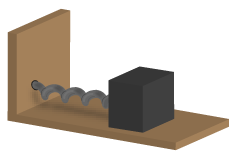
\includegraphics[width=\linewidth]{simple-spring}
\caption[A simple harmonic oscillator]{A simple harmonic oscillator: a mass $m$ on a frictionless surface attached to a  spring with force $F = -kx$.
\label{f.simple-spring}}
\end{marginfigure}

If we put the origin of our coordinate system where the mass is at rest with the spring relaxed, then the equation of motion of the mass is
\begin{equation}\label{e.SHO-basic}
	\DDtt{x} + \frac{k}{m} x = 0.
\end{equation}
You have solved this before: the most general solution is
\begin{equation}\label{e.SHO-general-solution}
	x(t) = x_{0}\cos(\wot) + \frac{v_{0}}{\omega_{0}}\sin(\wot)
\end{equation}
with $\omega_{0}^{2} = k/m$ and with $x_{0}$ and $v_{0}$ being the initial position and velocity of the mass.

\subsection{With driving at frequency $\omega \neq \omega_{0}$}

Now let's push on our mass with an oscillating force, $F\cos(\omega t)$ with $\omega\neq\omega_{0}$. A real world example would be holding a vibrating tuning fork near another fork tuned to a different frequency.  The equation of motion is now
\begin{equation}\label{e.SHO-driven}
	\DDtt{x} + \omega_{0}^{2}x = \frac{F}{m}\cos(\wt).
\end{equation}
You can verify by substitution that a general solution is
\[
	x(t) = \frac{F/m}{(\omega_{0}^{2}-\omega^{2})}\cos(\wt) + A\cos(\wot)+B\sin(\wot).
\]
Let's start with our harmonic oscillator at rest ($v_{0} = \left.\dif x/\dif t\right|_{t=0} = 0$) and at $\left. x\right|_{t=0} = 0$.  With these conditions, we can determine the constants $A$ and $B$; the solution is
\[
	x(t) = \frac{F/m}{(\omega_{0}^{2}-\omega^{2})}\left[\cos(\wt)-\cos(\wot)\right].
\]
Let's recast this by defining $\Delta = \omega_{0} - \omega$ and $\omega_{m} = (\omega_{0}+\omega)/2$.  Then
\begin{eqnarray*}
  \omega_{0}^{2}-\omega^{2} &=& (\omega_{0}-\omega)(\omega_{0}+\omega) = 2\Delta\omega_{m},\\
  \cos(\wot) &=& \cos\left(\wmt+\Delta t/2\right) = \cos(\wmt)\cos(\Delta t/2) - \sin(\wmt)\sin(\Delta t/2),\\
  \cos(\wt) &=& \cos\left(\wmt-\Delta t/2\right) = \cos(\wmt)\cos(\Delta t/2) + \sin(\wmt)\sin(\Delta t/2);
\end{eqnarray*}
and we write the solution as
\begin{equation}\label{e.beats}
	x(t) = \left[\frac{F/m}{\Delta\omega_{m}}\sin(\Delta t/2)\right]\sin(\wmt).
\end{equation}
This illustrates the phenomena of \textbf{beats}: the oscillation consists of a carrier signal at frequency $\omega_{m}$ with the amplitude modulated at the slower frequency $\Delta /2$.  Notice that the amplitude increases as $\Delta \to0$, i.e., $\omega\to\omega_{0}$.

\subsection{With both driving and damping}

Now let's make our model even more realistic by adding some \textbf{damping}.  We add a frictional force that is proportional to velocity, $F_{\mathrm{friction}} = -m\Gamma \dif x/\dif t$. Our complete equation of motion is then
\begin{equation}
	\DDtt{x} + \Gamma \DDt{x} + \omega_{0}^{2}x = \frac{F}{m}\cos(\omega t).
\end{equation}
The solution to this is straightforward to find, although the algebra is tedious (trust me on this). The general solution for initial conditions $\left.x\right|_{t=0} = x_{0}$ and $\left.\dif x/\dif t\right|_{t=0} = v_{0}$ is
\begin{eqnarray}
\label{e.general-solution-ddo}
\lefteqn{x(t) = \frac{F\womw/m}{\womw^{2}+\gw}\cos(\omega t)} && \\
	&+& \frac{\Gamma\omega F/m}{\womw^{2}+\gw}\sin(\omega t)\nonumber \\
	&+& \left[x_{0}-\frac{F\womw/m}{\womw^{2}+\gw}\right]{\color{red}e^{-\Gamma t/2}} \cos(\omega_{\Gamma}t) \nonumber\\
	&+& \left[\frac{v_{0}}{\omega_{\Gamma}}-\frac{\Gamma\omega F/m}{\womw^{2}+\gw}
	\,\frac{\omega}{\omega_{\Gamma}}\right]{\color{red}e^{-\Gamma t/2}} \sin(\omega_{\Gamma}t), 
	\nonumber
\end{eqnarray}
with
\[ 
    \omega_{\Gamma} = 
        \omega_{0}\left(1-\frac{\Gamma^{2}}{4\omega_{0}^{2}}\right)^{1/2}.
\]
Let's simplify this to the most relevant case.  First, the last two terms decay as {\color{red}$e^{-\Gamma t/2}$}: these are transients set by the initial conditions. After a time $2/\Gamma$ there will only be the first two terms, which oscillate at frequency $\omega$. 

We can simplify these first two terms even further: write
\[ \cos(\wt) = \frac{e^{i\wt}+e^{-i\wt}}{2},\quad \sin(\wt) 
    = \frac{e^{i\wt}-e^{-i\wt}}{2i}; \]
and combine terms to find
\begin{eqnarray}
    x(t) &=& \frac{F}{2m}\left[\frac{1}{\left(\omega_0^2-\omega^2\right) + i\Gamma\omega}\right]e^{i\wt} + \frac{F}{2m}\left[\frac{1}{\left(\omega_0^2-\omega^2\right) - i\Gamma\omega}\right]e^{-i\wt} \nonumber\\
    &=& \Re\left\{\frac{F}{m}\left[\frac{1}{\left(\omega_0^2-\omega^2\right) + i\Gamma\omega}\right]e^{i\wt}\right\}\label{e.oscillator-expression}
\end{eqnarray}
We use the symbol ``$\Re$'' to denote taking the real part of a complex quantity.  

From Eq.~(\ref{e.oscillator-expression}), we see that the oscillator can be described as the real part of a complex quantity $Ae^{i\wt}$, with
\[
    A = \frac{F}{m}\left[\frac{1}{\left(\omega_0^2-\omega^2\right) + i\Gamma\omega}\right].
\]
For $\omega \approx \omega_0$, we write $(\omega_0^2-\omega^2)\approx 2\omega_0(\omega_0-\omega)$ and take the square of the amplitude to find,
\begin{eqnarray}
    \left|A\right|^2 &=& \left(\frac{F}{2m\omega_0}\right)^2
        \frac{1}{(\omega_0-\omega)^2 + (\Gamma/2)^2}\nonumber\\
    &=& \frac{\pi}{2\Gamma}\left(\frac{F}{m\omega_0}\right)^2
        \left\{\frac{1}{\pi}\frac{\Gamma/2}{(\omega_0-\omega)^2 + (\Gamma/2)^2}\right\}
\end{eqnarray}
We rewrote the amplitude in the second line so that the term in $\{\cdot\}$ is normalized. The function
\[
    \mathcal{L}(\omega;\Gamma) = \frac{1}{\pi} 
        \frac{\Gamma/2}{(\omega_0-\omega)^2 + (\Gamma/2)^2}
\]
is known as a Lorentzian.  In contrast to a Gaussian, a Lorentzian is characterized by broad ``wings'' (Fig.~\ref{f.comparison}) as it goes to zero away from the central frequency $\omega_{0}$.
\begin{marginfigure}[-4\baselineskip]
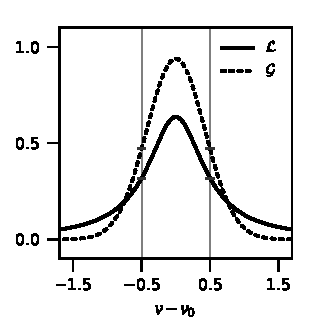
\includegraphics[width=\linewidth]{comparison}
\caption[Comparison of Lorentzian and Gaussian distributions]{\label{f.comparison}
Comparison of a Lorentzian ($\mathcal{L}$, solid line) and a Gaussian ($\mathcal{G}$, dotted line), both with $\mathrm{FWHM}=1$. The area under each curve is unity.}
\end{marginfigure}

\section{Atomic Lines}
You may be thinking, ``What does this have to do with atomic lines?'' Consider an electronic transition in an atom between two energy levels, $E_m$ and $E_n$. The natural frequency of this transition is $\nu_0 = |E_n-E_m|/h$. Light incident on the atom with frequency\sidenote{We are switching from angular frequency $\omega$ to frequency $\nu = \omega/2\pi$.} $\nu\neq\nu_0$ drives the electron at frequency $\nu$. An accelerating electron radiates, which damps the acceleration of the electron.  Classically, the transition in an atom is an electromagnetic oscillator with damping and driving terms, with cross-section\sidenote{For details, see the appendix.}
\begin{equation}\label{e.semi-classical}
    \sigma = \left(\frac{\pi e^2}{m_e c}\right)
    \left\{\frac{\Gamma/4\pi}{(\nu_0-\nu)^2 + (\Gamma/4\pi)^2}\right\}.
\end{equation}
The actual value of the cross-section must be calculated using quantum mechanics. The overall shape of the cross-section is still in the form of equation~(\ref{e.semi-classical}) with opacity
\begin{equation}
    \rho\kappa_\nu = n_i \left(\frac{\pi e^2}{m_e c}\right) f_{mn}
        \left\{\frac{\Gamma/4\pi}{(\nu_0-\nu)^2 + (\Gamma/4\pi)^2}\right\}.
\end{equation}
In this equation, $f_{mn}$ is a number, called the \emph{oscillator strength}, that results from the calculation of the transition probability from state $m$ to state $n$, and $n_i$ is the density of atoms in state $m$.  The key point is that $f_{mn}$ depends only on the details of the transition: the energies, spins, and parities of the atomic states.  It does not depend on environmental parameters such as temperature and pressure.  As a result, $f_{mn}$ can be measured or computed once and then tabulated.

There is an intrinsic width $\Gamma$ that is set by the finite lifetime of the energy levels; in practice, however, this is not important.  In a stellar atmosphere, the width $\Gamma$ is set by collisions.  For example, when an electron passes close by our atom, the electric field shifts the energy levels of the atom\sidenote{This is an application of the \emph{Stark} effect that you learn about in quantum mechanics.}.  The greater the collision rate, the larger the width.
If we have two stars of the same photospheric temperature (so that both stars have the same lines), then a way to increase the collision rate is to increase the pressure. Recall, however, that in the stellar atmosphere $P = (g/\kappa)\tau$; as a result, stars with a higher surface gravity will have broader lines. The inset in Figure~\ref{f.compare_grav} illustrates the broadening of the Balmer H$\gamma$ line ($5\to 2$) in the spectrum of a main-sequence A1 star compared with that of a supergiant A1 star.

\begin{figure}[hp]
    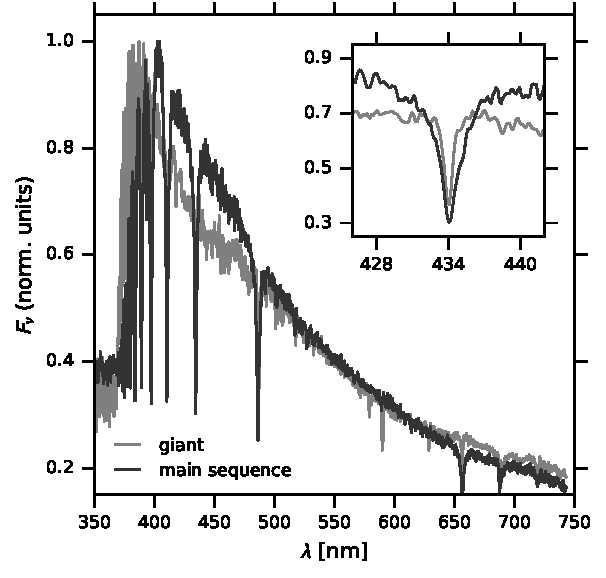
\includegraphics[width=\linewidth]{compare_grav}
    \caption[Spectra of two A1 stars]{\label{f.compare_grav}
    Spectra of two A1 stars, HD 16608 (a main sequence star) and SAO 12149 (a supergiant star).  Spectra are from \citet{Jacoby1984A-library-of-st}.
    }
\end{figure}

In addition to the width set by collisions, the line is also broadened by thermal motion: the atoms are in ceaseless motion; those headed towards us absorb at a blueshifted frequency, while those headed away from us absorb at a redshifted frequency.  Because the atomic velocities follow a Maxwell-Boltzmann distribution, the net effect is to make the core of the line (that is, near the center) assume a Gaussian profile.  Because a Gaussian falls off more quickly than a Lorentzian profile (see Fig.~\ref{f.comparison}), the wings of the line are still determined by the collision rate.

\section{A more detailed look}

This section is modified from Chapter 8 of \emph{Stellar Astrophyiscs}, \href{https://github.com/Open-Astrophysics-Bookshelf/stellar-physics-notes}{available} from The Open Astrophysics Bookshelf on GitHub.  In this section, Gaussian CGS units are used for the electromagnetic field. To convert to MKS, make the following substitutions:
\begin{eqnarray*}
e &\to& \frac{1}{\sqrt{4\pi\varepsilon_0}}e\\
\bvec{E} &\to& \sqrt{4\pi\varepsilon_0}\bvec{E}\\
c &\to& (\mu_0\varepsilon_0)^{-1/2}.
\end{eqnarray*}

\newthought{Suppose we have a classical charged harmonic oscillator.}  The instantaneous power emitted by the oscillator is
\begin{equation}\label{e.larmor-power}
	 P(t) = \frac{2}{3}\frac{e^{2}}{c^{3}} |\dot{\vu}|^{2},
\end{equation}
and when averaged over a cycle is
\begin{equation}\label{e.oscillator-power}
	 \left\langle P(t) \right\rangle = \frac{e^{2}}{3c^{3}}x_{0}^{2} \omega^{4},
\end{equation}
since $\dot{\vu} = -\omega^{2}\bvec{x}_{0}\cos \omega t$. Since the oscillator is radiating, it is losing energy and is damped. Let us write the damping as $\bvec{F}_{\mathrm{rad}}\vdot \vu$; to find $\bvec{F}_{\mathrm{rad}}$, we integrate the power loss over a cycle,
\[  -\int_{t_{1}}^{t_{2}}\!\dif t\;\frac{2}{3}\frac{e^{2}}{c^{3}}\dot{\vu}\vdot\dot{\vu} 
	= -\left.\frac{2}{3}\frac{e^{2}}{c^{3}}\dot{\vu}\vdot\vu\right|_{t_{1}}^{t_{2}} 
	+ \frac{2}{3}\frac{e^{2}}{c^{3}} \int_{t_{1}}^{t_{2}}\!\dif t\;\ddot{\vu}\vdot\vu. 
\]
Since the motion is periodic, the first term vanishes and we can therefore identify 
\[ 
	\bvec{F}_{\mathrm{rad}} = \frac{2}{3}\frac{e^{2}}{c^{3}}\ddot{\vu} 
	= -m\left(\frac{2e^{2}\omega^{2}}{3c^{3}m}\right)\vu
\]
as the radiation damping term with the term in parenthesis being the damping constant $\gamma$. 
If there is an driving electric field on our oscillator, then its equation of motion becomes
\begin{equation}\label{e.eq-sho}
	m\ddot{\bvec{x}} = -m\omega_{0}^{2}\bvec{x} + e\bvec{E}e^{i\omega t} - m\gamma \dot{\bvec{x}}.
\end{equation}
Using a trial function $\bvec{x}\propto e^{i\omega t}$ gives
\[
	\bvec{x} = \frac{e}{m}\frac{E e^{i\omega t}}{(\omega_{0}^{2}-\omega^{2}) + i\omega\gamma}.
\]
Taking the second derivative w.r.t.\ time of $\bvec{x}$, substituting into eq.~(\ref{e.larmor-power}), and averaging over a cycle gives the power radiated by the oscillator,
\[
	\left\langle P(t)\right\rangle = \frac{e^{4}\omega^{4} E^{2}}{3 c^{2}m^{2}}
	\frac{1}{(\omega_{0}^{2}-\omega^{2})^{2} + \gamma^{2}\omega^{2}}.
\]
Dividing $\langle P(t)\rangle$ by the incident power per unit area, $cE^{2}/(8\pi)$, gives the cross-section:
\begin{equation}\label{e.classical-oscillator-cross-section}
	\sigma = \frac{8\pi}{3}\frac{e^{4}}{m^{2}c^{3}}
	\frac{\omega^{4}}{(\omega_{0}^{2}-\omega^{2})^{2} + \gamma^{2}\omega^{2}}.
\end{equation}
Now, for $\omega \approx \omega_{0}$, we can expand $(\omega_{0}^{2}-\omega^{2})^{2} \approx 4\omega_{0}^{2}(\omega_{0}-\omega)^{2}$; furthermore, we identify $2e^{2}\omega_{0}^{2}/(3c^{3}m) = \gamma$ and equation~(\ref{e.classical-oscillator-cross-section}) becomes
\begin{equation}\label{e.cross-section-lorentz}
	\sigma = \pi\left(\frac{e^{2}}{mc}\right)\frac{\gamma}{(\omega_{0}-\omega)^{2} + (\gamma/2)^{2}}.
\end{equation}
The line profile is Lorentzian, with a width $\gamma$. In terms of wavelength, the width is
\[ 
	\Delta \lambda = \left|\frac{\dif\lambda}{\dif\omega}\right|\gamma = \frac{2\pi c}{\omega^{2}}\gamma
	= \val{\sci{1.2}{-4}}{\textrm{\AA}}.
\]
This width is independent of the transition frequency (it is just the classical electron radius), and it is very, very small.  In a stellar atmosphere, the width is set by interactions and doppler broadening.

\newthought{To understand how impacts affect the line width}, suppose we model the oscillator as being started and stopped by impacts; in between impacts it just goes as $e^{i\omega_{0}t}$.  To get the spectrum, we take the Fourier transform,
\[
	F(\omega,t) = \int_{0}^{t}\!\dif t'\; \exp[i(\omega_{0}-\omega)t'],
\]
where $t$ is some time between impacts. Now if the impacts are distributed randomly and are uncorrelated, then the distribution of wait times follows a Poisson distribution,
\[ W(t)\,\dif t = e^{-t/\tau}\,\dif t/\tau, \]
where $\tau$ is the average time between collisions.  Using this to compute the energy spectrum, we obtain
\[ E(\omega) = \frac{1}{2\pi\tau}\int_{0}^{\infty}\!\dif t\; F(\omega,t)F^{*}(\omega,t)W(t) = \frac{1}{\pi\tau} 
	\frac{1}{(\omega_{0}-\omega)^{2} + (1/\tau)^{2}};
\]
the line profile is again Lorentzian, with a FWHM $2/\tau$.

We might be inclined to treat the atoms as hard spheres, but this gives a large $\tau$, or equivalently a narrow line width. We are therefore led to consider longer-range interactions for setting the intrinsic line width. Table~\ref{t.perturbers} lists such interactions. For a given impact parameter, the interaction perturbs the energy levels; by integrating over a distribution of  impact parameters one gets the intrinsic damping. Of course, we should really use a quantum mechanical calculation.  We can scale our cross-section to the classical result (eq.~[\ref{e.cross-section-lorentz}]), however, by writing
\begin{equation}\label{e.cross-section}
	 \sigma_{\nu} = \left(\frac{\pi e^{2}}{m_{e}c}\right) f \phi_{\nu}, 
\end{equation}
where $\phi_{\nu}$ is the line profile (dimension $\sim \Hz^{-1}$) and $f$ is a dimensionless cross-section called the \textbf{oscillator strength}.

\begin{table}[htbp]
\caption{Interactions in stellar atmospheres}\label{t.perturbers}
\begin{tabular}{crcc}
\hline
perturbation & form & source & affects\\
\hline\hline
linear Stark & $C_{2} r^{-2}$ & $e^{-}$, $p$, ions & H (H$\alpha$, H$\beta$, \ldots)\\
quadratic Stark & $C_{4} r^{-4}$ & $e^{-}$ & non-hydrogenic ions\\
van der Waals & $C_{6}r^{-6}$ & atoms, H & most atomic lines, esp.\ in cool stars\\
\hline
\end{tabular}
\end{table}


\chapter{The Equation of State}\label{ch.degeneracy}
% !TEX root = ../intro-stellar-physics.tex

\newcommand*{\bra}[1]{\ensuremath{\left\langle#1\right|}}
\newcommand*{\ket}[1]{\ensuremath{\left|#1\right\rangle}}
\newcommand*{\braket}[2]{\ensuremath{\left\langle#1\right|\left.#2\right\rangle}}

\section{Degeneracy}
\label{s.degeneracy}

As a star contracts, the particles within it are packed ever closer together.  As we saw from our discussion of ionization, the behavior of particles must change when the separation between particles is of the order of the uncertainty in their positions.  Equivalently, our classical description breaks down when the particle density exceeds roughly
\begin{equation}\label{e.heuristic-quantum-density}
    \frac{1\;\textrm{particle}}{(\Delta x)^3} 
    = \left(\frac{\Delta p}{h}\right)^3 
    \sim \left(\frac{m\kB T}{h^2}\right)^{3/2}.
\end{equation}
Another way to put this is that quantum effects become important when there is roughly 1 particle in a normalized phase space volume $\dif^{3}x\,\dif^{3}p/h^{3}$.

Suppose we have two identical particles in a quantum state. Since the particles are identical, if we exchange them the wavefunction can only change by a phase factor\sidenote{See Box~\ref{sb.identical-particles}} $e^{i\delta}$. If we exchange the particles again, we are back to our original state; as a result, $e^{2i\delta} = 1$, and therefore $\delta = 0$ or $\pi$. Hence upon the exchange of particles, the wavefunction either is unchanged ($\delta=0$) or it changes sign ($e^{i\pi}=-1$).
\begin{quote}\itshape
    There are two types of particles in this world: those that change sign under exchange; and those that don't.
\end{quote}
Particles that don't change sign under exchange are called \newterm{bosons} and have integer spin. Photons are bosons. Particles that change sign under exchange are called \newterm{fermions} and have half-integer spin. Electrons, neutrinos, protons, and neutrons are all fermions. 

A consequence of the fermion wavefunction changing sign when any two particles are exchanged is that the wavefunction vanishes if any two particles are in the same state---that is, they have the same position, momentum, and spin. For spin-half particles like electrons, then means we can put at most two such electrons in the same position and momentum state; we do this by having their spins antiparallel.

\begin{sidebar}[Identical Particles]
\label{sb.identical-particles}
To understand how the interchange of identical particles works in more detail, let's start by recalling some features of quantum mechanics. This discussion is based on the treatment of \citet{Feynman1989The-Feynman-Lec}.
We denote a state as $\ket{a}$, where $a$ is just a label.  For example, $a$ could be "electron with such-and-such momentum".  The probability of finding the electron in some other state $\phi$ is given by $|\braket{\phi}{a}|^2$, where $\braket{\phi}{a}$ is a complex number known as the probability amplitude.

Now suppose we have two particles, a and b, and we scatter them so that one particle ends up in detector 1 and the other ends up in detector 2. There are two ways this can go, as shown here.
\begin{center}
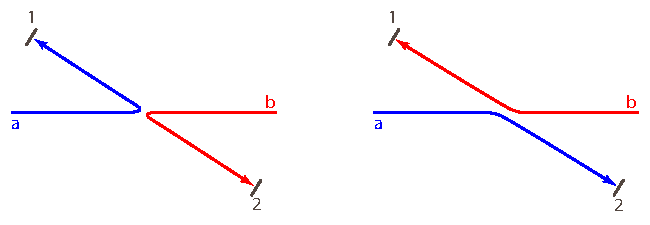
\includegraphics[width=\linewidth]{scattering-classical}
\end{center}
Classically, we would argue that the probability of getting either particle in detector 1 is just
\begin{equation}
    \mathcal{P}(\textrm{a or b in 1}) = \mathcal{P}(\textrm{a in 1}) + \mathcal{P}(\textrm{b in 1}).
\end{equation}
If particles a and b are different---e.g., one is a \carbon\ nucleus and the other is an \oxygen\ nucleus---then this holds in quantum mechanics as well. Quantum mechanically, we write
\begin{equation}
    \mathcal{P}(\textrm{a or b in 1}) = |\braket{1}{a}\braket{2}{b}|^2 + |\braket{2}{a}\braket{1}{b}|^2.
\end{equation}
If the particles are identical, however---for example, if a and b are two electrons with identical spin---then this picture is wrong.

Because of the uncertainty principle, we cannot follow the trajectories of a and b with infinite precision to see which is which; instead, the situation is more analogous to the depiction shown here.
\begin{center}
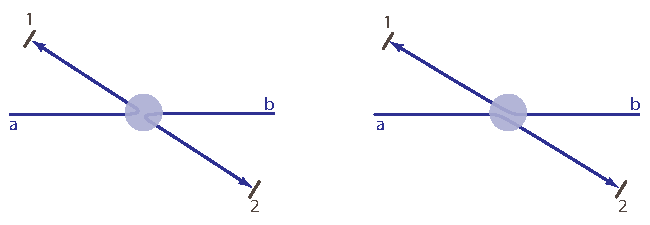
\includegraphics[width=\linewidth]{scattering-quantum}
\end{center}
There are now two indistinguishable ways of arriving at the final state---in this case, an electron in detector 1 and an electron in detector 2. According to quantum mechanics, we must therefore sum the amplitudes for getting to the final state, \emph{before taking the square}. That is, the probability for this one particle to end up in detector 1 and the other to end up in detector 2 is
\begin{eqnarray}
    \mathcal{P}(\textrm{a or b in 1}) &=& |\braket{1}{a}\braket{2}{b} + \braket{2}{a}\braket{1}{b}|^2\nonumber\\
    &=& |\braket{1}{a}\braket{2}{b}|^2 + |\braket{2}{a}\braket{1}{b}|^2 \nonumber\\
    && + {\color{red}\left[ \braket{1}{a}^*\braket{2}{b}^*\braket{2}{a}\braket{1}{b}\right.} \nonumber\\
    && {\color{red}+ \left.\braket{2}{a}^*\braket{1}{b}^*\braket{1}{a}\braket{2}{b}\right]} \nonumber\\
    &=& \mathcal{P}(\textrm{a in 1}) + \mathcal{P}(\textrm{b in 1}) \nonumber\\
    && + {\color{red}\left[ \braket{1}{a}^*\braket{2}{b}^*\braket{2}{a}\braket{1}{b}\right.}\nonumber\\
    && {\color{red}+ \left.\braket{2}{a}^*\braket{1}{b}^*\braket{1}{a}\braket{2}{b}\right]}.
    \label{e.scattering-quantum}
\end{eqnarray}
The probability of scattering an electron into detector 1 is the classical value plus the \emph{additional} interference term in $\color{red}[\cdot]$.

\newthought{To see the effect on the thermal properties,} let's imagine putting two particles into the same small volume.  To do this, we imagine the detectors 1 and 2 sliding together until they overlap, as shown here.  
\begin{center}
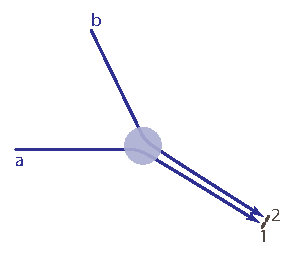
\includegraphics{fermions}
\end{center}
Since detectors 1 and 2 are approaching one another, we must have that
\begin{equation}
    |\braket{1}{a}\braket{2}{b}|^2 = |\braket{2}{a}\braket{1}{b}|^2.
\end{equation}
This does not imply, however, that $\braket{1}{a}\braket{2}{b} = \braket{2}{a}\braket{1}{b}$: the amplitudes could differ by a phase factor, so that interchanging the particles would yield
\[
    \braket{2}{a}\braket{1}{b} = e^{i\delta}\braket{1}{a}\braket{2}{b}.
\]
If we interchange the particles, and then interchange them again, we get
\[
    \braket{1}{a}\braket{2}{b} = e^{2i\delta}\braket{1}{a}\braket{2}{b};
\]
since swapping the particles twice just gets up back to the original situation, we must have that $e^{i\delta} = \pm 1$.

If there is no change of sign, i.e., $\braket{2}{a}\braket{1}{b} = \braket{1}{a}\braket{2}{b}$, then from equation~(\ref{e.scattering-quantum}) we have
\begin{equation}\label{e.boson}
    \mathcal{P}(\textrm{a or b in 1}) = 2|\braket{1}{a}\braket{2}{b}|^2 + 2|\braket{2}{a}\braket{1}{b}|^2.
\end{equation}
This is \emph{twice} the classical value: the probability of the particles entering the same state is enhanced.

In contrast, if $\braket{2}{a}\braket{1}{b} = -\braket{1}{a}\braket{2}{b}$, then equation~(\ref{e.scattering-quantum}) implies that
\begin{eqnarray}
\mathcal{P}(\textrm{a or b in 1}) &=& |\braket{1}{a}\braket{2}{b}| + |\braket{2}{a}\braket{1}{b}| \nonumber\\ 
    && - |\braket{1}{a}\braket{2}{b}| - |\braket{2}{a}\braket{1}{b}| \nonumber\\ 
    &=& 0.\label{e.fermion}
\end{eqnarray}
\begin{quote}\itshape
We cannot have 2 identical particles with the same momentum, position, and spin if their wavefunction changes sign when the particles are exchanged.
\end{quote}
Particles with integer spin (i.e., their angular momentum is an integer multiple of $\hbar$) have wavefunctions that do not change sign under exchange; these particles are said to obey \emph{Bose-Einstein statistics} and are called \emph{bosons}.  Particles with half-integer spin have wavefunctions that do change sign under exchange; these particles are said to obey \emph{Fermi-Dirac statistics} and are called \emph{fermions}.  Photons are bosons; electrons, protons, neutrons, and neutrinos are fermions.
\end{sidebar}

\newthought{To connect with the equation of state,} we begin by imagining a small volume containing $N$ electrons. Motivated by eq.~(\ref{e.heuristic-quantum-density}), we divide the phase space into cells,
\[
	\frac{\dif^{3}x\,\dif^{3}p}{h^{3}},
\]
and into each cell we place 2 electrons with opposing spins. We always add the electrons to the lowest open energy level, and repeat the process until we have added all $N$ electrons. This procedure is represented by the equation
\begin{equation}
	N = \frac{2}{h^{3}}\int_{V}\dif^{3}x\int_{0}^{\EF}\dif^{3}p
\end{equation}
In this equation $\EF$, the \emph{Fermi energy}, is the energy of the last electrons added and is the largest filled energy level.

If our volume is isotropic, then we can change variables: first, to spherical momentum coordinates, $\dif^{3}p = 4\pi p^{2}\,\dif p$; second, from $\dif p$ to $\dif\varepsilon$.  Since $p = \sqrt{2m\varepsilon}$, where $\varepsilon$ is the energy of a single electron,
\[
	\dif p = \sqrt{\frac{m}{2\varepsilon}}\,\dif \varepsilon;
\]
we can therefore change variables and integrate over $\varepsilon$ from $0$ to $\EF$ to obtain
\[
	N = \frac{8\pi}{h^{3}}V \int_{0}^{\EF} \sqrt{2}m^{3/2}\varepsilon^{1/2}\,\dif \varepsilon
	= \frac{8\pi}{3h^{3}} V (2m)^{3/2} \EF^{3/2}.
\]
Solving for the Fermi energy gives
\begin{equation}\label{e.fermi-energy}
	\EF = \frac{h^{2}}{2m}\left(\frac{3}{8\pi}\frac{N}{V}\right)^{2/3}.
\end{equation}
What is the total energy of our system? We again integrate over phase space, with each electron multiplied by its energy $\varepsilon$:
\begin{equation}\label{e.total-energy}
	E = \frac{8\pi}{h^{3}}V\int_{0}^{\EF}\sqrt{2}m^{3/2}\varepsilon^{3/2}\,\dif\varepsilon = \frac{8\pi}{5h^{3}}V(2m)^{3/2} \EF^{5/2}.
\end{equation}
Using eq.~(\ref{e.fermi-energy}) to substitute for $\EF$ in eq.~(\ref{e.total-energy}), we can find the energy per unit volume,
\[
	\frac{E}{V} = \frac{3}{5}\left(\frac{3}{8\pi}\right)^{2/3}\frac{h^{2}}{2m}n^{5/3} = \frac{3}{5} n \EF,
\]
where $n=N/V$ is the density of electrons.

Recall that for a non-relativistic gas the pressure is $P = (2/3)(E/V)$.  Hence the pressure of our electron gas is
\begin{equation}\label{e.pressure-electrons}
	P = \frac{2}{3}\frac{E}{V} = \frac{2}{5} n\EF
		= \frac{2}{5}\left(\frac{3}{8\pi}\right)^{2/3}\frac{h^{2}}{2m}n^{5/3}.
\end{equation}
Notice that the pressure is independent of the temperature.


\chapter{Convection}\label{ch.convection}
% !TEX root = ../intro-stellar-physics.tex

Hot air rises, as a glider pilot or hawk can tell you. The fluid velocities in question are very subsonic, so we have hydrostatic equilibrium to excellent approximation. But the fluid motions make an enormous difference for heat transport! This state of fluid motions induced by a temperature gradient is known as \newterm{convection}. You can perform the following demonstration of the onset of convection.  Brew tea, and pour the hot tea into a saucepan that is on an unlit burner.  Use a straw with your thumb over the top to insert a layer of cold milk under the warm tea in the saucepan.  The temperature difference between the tea and milk will inhibit their mixing. Light the burner, and watch for the development of convection---you will know it when you see it.

\begin{figure}[htbp]
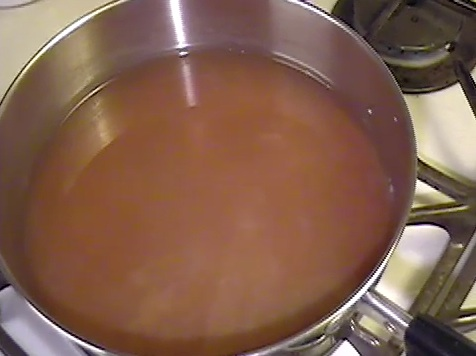
\includegraphics[width=0.5\linewidth]{convection-1}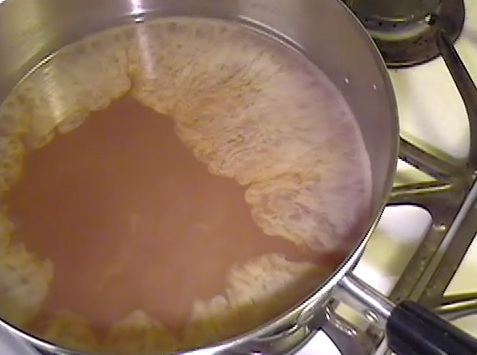
\includegraphics[width=0.5\linewidth]{convection-2}
\caption{Onset of convection in a tea-milk mixture.\label{f.tea}}
\end{figure}

\section{The adiabatic thermal gradient}\label{s.adiabatic-gradient}

We saw that the temperature gradient in the star is
\begin{equation}
    \label{e.gradient-temperature}
    \DD{T}{r} = -\frac{3\rho\kappa}{4acT^3}\frac{L(r)}{4\pi r^2}.
\end{equation}
Here $\kappa$ is the opacity and $L(r)$ is the luminosity at radius $r$: $L/4\pi r^2$ is the flux. If this thermal gradient, $|\dif T/\dif r|$, becomes too large, however, the fluid becomes unstable: warm fluid begins to rise while cold fluid sinks to take its places.  This usually occurs quickly enough that there is little exchange of heat between the upwelling warm current and the sinking cold one.

As a result of this lack of heat exchange, the motions are termed \newterm{adiabatic}.  To understand what this means, recall the first law of thermodynamics\cite{Fermi1956Thermodynamics}, which relates the change in internal energy $\dif U$ and in volume $\dif V$ to the heat transferred $\dif Q$:
\begin{equation}\label{e.first-law-thermo}
	\dif Q = \dif U + P\dif V,
\end{equation}
where $P$ is the pressure. Now, we aren't using volume to describe our fluid so let's apply this equation to a fixed mass of fluid, say $m = \val{1}{\kilo\gram}$, and divide both sides of Equation~(\ref{e.first-law-thermo-astro}) by the mass. Then $Q$ refers to the heat transferred \emph{per kilogram}, and $U$ refers to the internal energy \emph{per kilogram}.  Instead of $\dif V$, we then have $\dif(V/m) = \dif(1/\rho) = -\rho^{-2}\dif\rho$.  Our first law, rewritten in terms of mass-specific quantities, is thus
\begin{equation}\label{e.first-law-thermo-astro}
	\dif Q = \dif U -\frac{P}{\rho^{2}}\dif \rho.
\end{equation}
Suppose we wish to express quantities in terms of temperature $T$ and density $\rho$: then
\[ \dif U = \tderiv{U}{T}{\rho}\dif T + \tderiv{U}{\rho}{T}\dif \rho, \]
and
\[ \dif Q = \tderiv{U}{T}{\rho}\dif T + \left[\tderiv{U}{\rho}{T} - \frac{P}{\rho^{2}}\right]\dif \rho. \]
Hence the heat needed to raise the temperature of one kilogram of fluid when holding density fixed is
\begin{equation}\label{e.CV}
C_{\rho} \equiv \tderiv{Q}{T}{\rho} = \tderiv{U}{T}{\rho}.
\end{equation}
For an ideal gas, $U = U(T)$ and $C_{\rho}$ is approximately constant; hence we may integrate equation~(\ref{e.CV}) to obtain $U = C_{\rho}T + \textrm{const}$.

In Eq.~(\ref{e.first-law-thermo-astro}), the last term is $-(P/\rho)\, (\dif\rho/\rho) = -(P/\rho)\,\dif\ln\rho$. This demonstrates a useful trick: take the logarithm of the equation of state, $\ln (P) = \ln(\rho) + \ln (T) + \ln (\kB/\mu\mb)$, and then take the differential to obtain
\[ \frac{\dif P}{P} = \frac{\dif\rho}{\rho} + \frac{\dif T}{T}. \]
Now eliminate $\dif\rho/\rho$ in the equation
\[ \dif Q = C_{\rho}\dif T - \frac{P}{\rho}\frac{\dif\rho}{\rho} \]
to obtain an expression for the heat transferred as a function of temperature and pressure,
\[ \dif Q = \left[C_{\rho} + \frac{P}{\rho T}\right]\dif T - \frac{1}{\rho}\dif P
	 = \left[C_{\rho} + \frac{\kB}{\mu\mb}\right]\dif T - \frac{1}{\rho}\dif P. \]
From this we see that the heat needed to raise the temperature of one kilogram when holding pressure fixed is
\begin{equation}\label{e.CP}
C_{P}\equiv \tderiv{Q}{T}{P} = C_{\rho} + \frac{\kB}{\mu\mb}.
\end{equation}
For a plasma of ions and electrons, $C_\rho = (3/2)\kB/(\mu\mb)$ and hence $C_P = (5/2)\kB/(\mu\mb)$.  The ratio of specific heats is
\begin{equation}\label{e.gamma}
    \gamma = \frac{C_P}{C_\rho} = \frac{5/2}{3/2} = \frac{5}{3}.
\end{equation}
This value of $\gamma$ is for an ideal gas and does not hold universally.

\newthought{During adiabatic motion, there is no heat exchange:} hence, the entropy is constant,
\begin{equation}\label{e.differential-entropy}
    T\dif S = \dif Q = 0 = C_{P}\dif T - \frac{1}{\rho} \dif P.
\end{equation}
Using the ideal gas equation of state we can write 
\[
    \frac{1}{\rho} = \frac{\kB}{\mu\mb} \frac{T}{P}
\]
and insert this into Equation~(\ref{e.differential-entropy}) to obtain
\begin{equation}\label{e.differential-adiabat}
     \frac{\dif T}{T} = \frac{\kB/(\mu\mb)}{C_{P}}\frac{\dif P}{P} = \frac{C_{P}-C_{\rho}}{C_{P}} \frac{\dif P}{P} = \frac{\gamma-1}{\gamma}\frac{\dif P}{P}.
\end{equation}
Integrating both sides of the equation gives
\[ \ln T = \frac{\gamma-1}{\gamma}\ln P + \textrm{const.},\]
or 
\begin{equation}\label{e.adiabat}
 T = T_{0}\left(\frac{P}{P_{0}}\right)^{(\gamma-1)/\gamma},
\end{equation}
where $T_{0}$ and $P_{0}$ are the temperature and pressure at the beginning of the adiabatic process.
Equation~(\ref{e.adiabat}) tells us how the temperature changes with pressure along an adiabat for an ideal gas.  Notice that we can recast Equation~(\ref{e.differential-adiabat}) as
\begin{equation}
    \frac{P}{T}\left(\dd{T}{P}\right)_s = \left(\dd{\ln T}{\ln P}\right)_s = \frac{\gamma-1}{\gamma}.
\label{e.nabla-adiabat}
\end{equation}
Equation~(\ref{e.nabla-adiabat}) tells us how temperature changes with pressure in an adiabatically stratified gas.

\section{The onset of convection}\label{s.convection-onset}

To understand when convection starts, let's consider a fluid in planar geometry and hydrostatic equilibrium,
\begin{equation}
\frac{\dif P}{\dif r} = -\rho g.
\end{equation}
Now, imagine moving a blob of fluid upwards from $r$ to $r+h$.  We move the blob slowly enough that it is in hydrostatic equilibrium with its new surroundings, $P_{b}(r+h) = P(r+h)$, where the subscript $b$ refers to ``blob.'' We do move the blob quickly enough, however,  that it does not remain in \emph{thermal} equilibrium with its surroundings; that is, we move the blob \emph{adiabatically}.  The entropy of the blob is therefore constant, 
$S_{b}(r+h) = S_{b}(r) = S(r)$, and is therefore not, in general, equal to the entropy of the surrounding gas at $r+h$: $S_{b}(r+h)  \neq S(r+h)$.  

As the blob rises, it displaces some of the surrounding fluid. Archimedes tells us that if the displaced fluid is less massive than the blob, then the blob will sink.  We can rephrase this in terms of the volume occupied by a unit mass of fluid $V$: if the volume occupied by the blob is less than the volume of an equal mass of background, then the blob will sink. Translating this into an equation: if
\begin{eqnarray}
\lefteqn{V[P(r+h),S(r+h)] - V_{b}[P_{b}(r+h),S_{b}(r+h)] =}\nonumber\\
&&  V[P(r+h),S(r+h)] - V[P(r+h),S(r)] > 0
\label{e.archimedes}
\end{eqnarray}
then the blob will sink. If condition (\ref{e.archimedes}) is violated, the blob will continue to rise, and the system is unstable to convection.  
Figure~\ref{f.convective-schematic} has a cartoon of this process.

\begin{marginfigure}
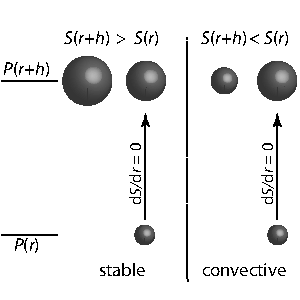
\includegraphics[width=\textwidth]{convective}
\caption[Illustration of criteria for convective instability.]{\label{f.convective-schematic}Illustration of criteria for convective instability.  On the left, raising a blob a distance $h$ adiabatically and in pressure balance with its surrounding results in a higher density $V_{b} < V$.  This is stable: the blob will sink back.  On the right, the blob is less dense and hence buoyant: it will continue to rise.}
\end{marginfigure}

Taking $h$ to be an infinitesimal displacement and expanding the left-hand side of equation~(\ref{e.archimedes}) gives us a local condition for stability:
\begin{equation}\label{e.convective-stability}
V[P(r+h),S(r)] + \tderiv{V}{S}{P}\frac{\dif S}{\dif r} - V[P(r+h),S(r)]  = \tderiv{V}{S}{P}\frac{\dif S}{\dif r} > 0 .
\end{equation}
Noting that
\begin{eqnarray*}
\tderiv{V}{T}{P} &=& \tderiv{V}{S}{P}\tderiv{S}{T}{P}\\
 &=& \frac{C_{P}}{T}\tderiv{V}{S}{P},
 \end{eqnarray*}
 we can rewrite equation~(\ref{e.convective-stability}) as
 \[
 \frac{T}{C_{P}}\tderiv{V}{T}{P}\frac{\dif S}{\dif r} > 0.
 \]
Now, $(\partial V/\partial T)_{P}$ is positive (gas expands on being heated), so our condition for stability is simply
 \begin{equation}\label{e.entropy-condition}
\frac{\dif S}{\dif r} > 0.
\end{equation}
In a convectively stable star, the entropy must increase with radius. if $\dif S/\dif r < 0$, then convection occurs and carries high-entropy material outward, where it will eventually mix with the ambient medium.  As a result, convection drives the entropy gradient toward the marginally stable configuration $\dif S/\dif r = 0$.  If a star is fully convective and mixes efficiently, then the interior of the star lies along an adiabat. 

\newthought{We can derive a condition for convective stability} in terms of the local gradients of temperature and pressure. Writing $S = S[P(r),T(r)]$ we expand equation~(\ref{e.entropy-condition}) to obtain
\begin{equation}\label{e.schwarzschild-1}
\frac{\dif S}{\dif r} = \tderiv{S}{P}{T} \frac{\dif P}{\dif r} + \tderiv{S}{T}{P}\frac{\dif T}{\dif r} .
\end{equation}
Now, $P$ is a monotonically decreasing function of $r$, which means we can change variables:
\begin{equation}\label{e.TPstar}
\frac{\dif T}{\dif r} = \TPstar \frac{\dif P}{\dif r} .
\end{equation}
Here $\dif T/\dif P|_{\star}$ is the slope of the $T(P)$ relation \emph{for the stellar interior}.  In particular, this is \emph{not} a thermodynamic equality. Substituting equation~(\ref{e.TPstar}) into equation~(\ref{e.schwarzschild-1}), using hydrostatic equilibrium to eliminate $\dif P/\dif r$, and recognizing that $(\partial S/\partial T)_{P} = C_{P}/T$, we obtain
\begin{equation}\label{e.schwarzschild-2}
\frac{\dif S}{\dif r} =  -\rho g\left[\tderiv{S}{P}{T} + \frac{C_{P}}{T} \TPstar \right].
\end{equation}
Finally, we can use the identity
\begin{equation}
\tderiv{S}{P}{T}\tderiv{T}{S}{P}\tderiv{P}{T}{S} = -1
\end{equation}
to simplify equation~(\ref{e.schwarzschild-2}),
\begin{equation}
\frac{\dif S}{\dif r} = -\frac{\rho g}{P}C_{P}\left[\frac{P}{T}\TPstar - \frac{P}{T}\tderiv{T}{P}{S}\right].
 \label{e.schwarzschild}
\end{equation}
Hence, if the term in $\left[\cdot\right]$ is positive, then the fluid is convectively unstable.

Let's use our expression for the flux, Equation~(\ref{e.gradient-temperature}), to put $\left.\dif T/\dif P\right|_\star$ in terms of $\kappa$ and $L(r)$:
\begin{eqnarray}
    \frac{P}{T}\TPstar &=& \frac{P}{T}\DD{T}{r}\DD{r}{P} = \frac{P}{\rho g(r)}\frac{1}{\color{red}T}\frac{{\color{red}3}\rho\kappa}{4c {\color{red}a T^3}}\frac{L(r)}{4\pi r^2} \nonumber\\
    &=& \frac{P}{\color{red}\Prad}\frac{\kappa}{16\pi Gc} \frac{L(r)}{m(r)}.
\end{eqnarray}
The fluid is unstable to convection if
\begin{equation}
    \frac{P}{\Prad}\frac{\kappa}{16\pi Gc}\frac{L(r)}{m(r)} > \tderiv{\ln T}{\ln P}{S}  = \frac{\gamma -1}{\gamma}.
\end{equation}
We have used Equation~(\ref{e.nabla-adiabat}) for the last term here.
This occurs for large $\kappa$ (outer layers of cool stars) or for a high $L(r)/m(r)$ (centers of luminous hot stars).  On the main-sequence, stars with $M \lesssim \Msun$ have convective outer layers; stars with $M \lesssim \val{0.3}{\Msun}$ are fully convective. Stars with $M\gtrsim\Msun$ have convective cores.

\chapter{Non-resonant Fusion Reactions}\label{ch.nuclear-burning}
% !TEX root = ../intro-stellar-physics.tex

\section{The nucleus}

Experimentally, nuclei are on the order of femtometers\sidenote{Sometimes called a \emph{Fermi}} ($\val{1}{\fermi} = \val{10^{-15}}{\meter}$) in size. Like an atom, the nucleus also has excited states; typical energies for these are on the order of MeV ($\val{1}{\MeV} = \val{10^{6}}{\eV}$). \marginnote{An \newterm{electron volt} (eV) is the energy acquired by an electron being accelerated through a potential difference of 1 volt.} It therefore makes sense to use fm and MeV as our units of length and energy. In these units, the combination
\[	\hbar c = \val{197}{\MeV\,\fermi} \]
to three significant figures. In quantum field theory, the strength of the electromagnetic interaction is characterized by the dimensionless \newterm{fine structure constant}
\[	\alphaF = \frac{e^{2}}{4\pi\epsilon_{0}\hbar c} = \frac{1}{137}, \]
again to three significant figures. From these two quantities, we find the electron (or proton) charge in these units,
\[
	\frac{e^{2}}{4\pi\epsilon_{0}} = \alphaF\hbar c = \val{1.44}{\MeV\,\fermi}.
\]
Put another way, the potential energy between two protons of charge $e$ separated by $\val{1}{\fermi}$ is $\val{1.44}{\MeV}$.

The strong nuclear force differs from electromagnetism and gravity in several ways. First, the strong nuclear force is short-range: the interaction vanishes for distances $\gtrsim\val{2}{\fermi}$. It is weakly attractive for distances $\val{1}{\fermi}\lesssim r\lesssim\val{2}{\fermi}$ and becomes strongly repulsive at distances $\ll\val{1}{\fermi}$. The potential between the neutron and proton in a deuterium (\hydrogen[2]) nucleus (called a deuteron) therefore looks something like that sketched in Fig.~\ref{f.nuclear-potential}. The deuteron's ground state (black dotted line) is at $E_{\mathrm{d}} = -\val{2.2}{\MeV}$, so the nucleus is weakly bound ($|E_{\mathrm{d}}| \ll |V|$, where $V$ is the depth of the potential well).

\begin{marginfigure}[-8\baselineskip]
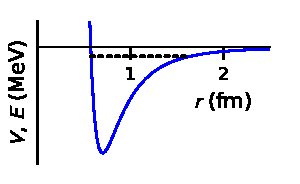
\includegraphics[width=\linewidth]{nuclear-potential}
\caption[Schematic of the nuclear potential]{\label{f.nuclear-potential}Schematic of the nuclear potential for a deuteron (\hydrogen[2]). The binding energy of the deuteron is shown as a black dotted line.}
\end{marginfigure}

\begin{exercisebox}[Depth of nuclear well]
We can estimate the depth of the well in Fig.~\ref{f.nuclear-potential}. Since this is a two-body problem, transfer to center-of-mass coordinates and treat this as a single particle with a reduced mass $m_{p}m_{n}/(m_{p}+m_{n}) \approx m_{n}/2$. Use the uncertainty principle, with $\Delta x$ being the width of the well, to get an estimate of $p\sim\Delta p$ and from this estimate the kinetic energy of the particle. Finally, use the small value of the binding energy (sum of potential and kinetic energies) to estimate the depth of the potential well.
\end{exercisebox}

Also unlike electromagnetism and gravity, the strong nuclear force does not obey superposition: we cannot write the energy of the nucleus as a sum over the potential between all pairs of nucleons. Moreover, the strong nuclear force is not a central force, meaning that it depends on more than just the distance between any two nucleons. The behavior of an atomic nucleus is thus much more complicated to describe than the electronic structure of the atom.

\newthought{Despite these complications, we can construct a phenomenological formula for the nuclear mass that is reasonably accurate.} Let us write the mass of a nucleus with $A$ nucleons---$Z$ protons and $N=A-Z$ neutrons---as
\[
	M(Z,N) = Zm_{p} + Nm_{n} - B(Z,N)/c^{2},
\]
where $B(Z,N)$ is the \newterm{binding energy}---the amount of energy that must be supplied to the nucleus in order to break it into its constituent protons and neutrons.
Because the nuclear force is weakly attractive for separations $\val{1}{\fermi}\lesssim r\lesssim\val{2}{\fermi}$ and repulsive at shorter distances (Fig.~\ref{f.nuclear-potential}), there is a characteristic spacing between nucleons that is a bit larger than $\val{1}{\fermi}$. In a large nucleus, we therefore expect the nucleons to have a roughly constant density, so that the volume of the nucleus is proportional to $A$; experimentally, the radius of the nucleus is roughly\sidenote{The value of the radius depends on how it is measured; scattering with various light particles (protons, neutrons, alpha, electrons) agree, however, that $r_{A}\propto A^{1/3}$.}
\[
	r_{A} = \valrng{1.1}{1.8}{\fermi}\times A^{1/3}.
\]
Notice that because the nucleon-nucleon potential is short-ranged, nucleons in a large nucleus only interact with their nearest neighbors. Indeed the nucleon-nucleon interaction in similar in form to the potential between molecules in a fluid, such as a water drop. This motivates developing a simple formula that gives a decent approximation for the binding energy. For the first term, we estimate the binding energy of a large nucleus as the binding energy of a single nucleon with its neighbors, multiplied by the number of nucleons. Experimentally, it is found that for large nuclei this is the case: the binding energy per nucleon is roughly constant: we say that the nuclear interaction \newterm{saturates}, so that $B(Z,N) \propto A = (Z+N)$.

\begin{exercisebox}[If the strong force were long-range]
To see how the nuclear force differs from the long-range Coulomb and gravitational force, suppose instead that the nuclear force acted like a super-gravity. Use the results from our constant-density model of a star (eq.~[\ref{e.energy-constant-density-sphere}]) to derive how the binding energy would scale with $A$ in this case.
\end{exercisebox}

It is energetically favorable to have equal numbers of neutrons and protons. We therefore define an asymmetry parameter $\eta \equiv (N-Z)/(N+Z) = 1-2Z/A$, so that $-1\le\eta\le1$. The nuclear contribution to the binding energy is maximized for $\eta = 0$ (equal numbers of protons and neutrons). Because the nuclear force does not distinguish between neutrons and protons, the binding energy is quadratic in $\eta$, so that $B$ doesn't depend on the sign of $\eta$. Thus our first approximation for the binding energy is $B \approx (a_{V} - a_{A}\eta^{2}) A$. Here $a_{V}$ and $a_{A}$ are as-yet-undetermined coefficients.

In a fluid drop there is a correction for the surface tension. Heuristically, we imagine that nuclei in the surface have fewer neighbors and are therefore not as bound. We therefore subtract from our formula a term proportional to the surface area, $\propto r_{A}^{2} \propto A^{2/3}$. The next iteration of our liquid-drop approximation is thus $B \approx (a_{V}- a_{A}\eta^{2})A - a_{S}A^{2/3} $.

Finally, the protons in the nucleus are charged and therefore repel one another. This Coulomb repulsion also reduces the binding energy. We therefore subtract a term $\propto Z^{2}/r_{A}\propto Z^{2}/A^{1/3}$ from our mass formula to obtain
\begin{equation}\label{e.liquid-drop}
B = \left(a_{V} -a_{A}\eta^{2}\right) A -  a_{S}A^{2/3} - a_{C} \frac{Z^{2}}{A^{1/3}}. 
\end{equation}
This is a version of the \newterm{semi-empirical mass formula}, also known as the \newterm{Bethe-Weizs\"acker mass formula}.
The coefficients $a_{V},a_{A},a_{S},a_{C}$ are found by fitting the formula to known nuclear masses\sidenote{This fit should have another term to account for the pairing of neutrons and protons, so that the binding energy is  increased for even $Z$ and $N$. We omit that term here for simplicity.}
for measured nuclear masses (Table~\ref{t.liquid-drop}).
\begin{margintable}
\caption[Liquid-drop coefficients]{\label{t.liquid-drop} Coefficients for hte fit to nuclear masses, (\protect\ref{e.liquid-drop}), in units of MeV.}
\begin{tabular}{rrrr}
$a_V$ & $a_A$ & $a_S$ & $a_C$ \\
\hline
15.5 & 22.7 & 16.6 & 0.71\\
\end{tabular}
\end{margintable}

\begin{exercisebox}[The nuclear landscape]
For a given nuclear mass number $A$, derive an expression for the charge number $Z_{\star}(A)$ that maximizes the binding energy (eq.~[\ref{e.liquid-drop}] with coefficients from Table~\ref{t.liquid-drop}).
\begin{enumerate}
\item Plot the ratio $Z_{\star}/A$ for $4\le A\le 128$. Give a physical explanation for the behavior of $Z_{\star}/A$.
\item Plot the binding energy per nucleon $B/A$ as a function of $Z_{\star}$ and $A$, for $4\le A\le 128$.
\item Find the atomic number $Z$ and atomic mass $A$ of the nucleus with the maximum $B/A$.
\end{enumerate}
\end{exercisebox}

\section{Nuclear reactions}

From mass-energy conservation, the heat evolved during a nuclear reaction equals the change in mass of the reacting system. For example, in the reaction
\[
	\helium[3] + \helium[3] \to \helium + \pt + \pt,
\]
the change in mass is
\begin{eqnarray*}
	\lefteqn{2\left[2m_{p}+m_{n}-B(\helium[3])\right] - \left[2m_{p}+2m_{n}-B(\helium)\right] - 2m_{p}} \\
	&=& B(\helium)-B(\helium[3])\\
	&=& \val{28.296}{\MeV} - \val{7.718}{\MeV}\\ &=& \val{20.578}{\MeV}.
\end{eqnarray*}

\begin{exercisebox}[Heat from hydrogen fusing to helium]
Fusion of hydrogen into helium entails converting 4 hydrogen atoms (including the 4 electrons) into 1 helium atom (2 protons, 2 neutrons, 2 electrons) with $B = \val{28.296}{\MeV}$. What is the heat evolved \emph{per hydrogen atom}? Assume that the sun has been shining with its current luminosity over its life. What mass of hydrogen atoms would need to undergo fusion to supply this energy? How large is this mass relative to the total mass of the sun? 
\end{exercisebox}

\newthought{You might at first think that because the nuclear interaction is short-range, the cross-section is something like $\pi r_{n}^{2}$, where $r_{n}\approx\valrng[--]{1}{2}{\fermi}$.} Things are a bit more subtle, however, and in this section we are going to take the reaction-rate apart to understand how it works. First, the ``size'' of a particle is in general proportional to the ``size'' of the wavefunction, which is set by the uncertainty principle, 
\[\pi\left(\frac{\lambda}{2\pi}\right)^{2} = \pi \left(\frac{\hbar}{p}\right)^{2} = \pi\frac{\hbar^{2}}{2mE}.\]
Notice that if we multiply and divide by $c^{2}$, then we can estimate the area as
\[
	\frac{(\hbar c)^{2}}{m_{p} c^{2}} \frac{1}{E} \sim \val{\sci{4}{4}}{\fermi^{2}} \times \left(\frac{\keV}{E}\right) = \val{400}{\barn}\left(\frac{\keV}{E}\right).
\]	
Here we've introduced a convenient unit for cross-sections, the \newterm{barn}\sidenote{as in hitting the broad side of}, with $\val{1}{\barn} = \val{10^{-28}}{\meter^{2}} = \val{100}{\fermi^{2}}$.

The key point is that the size of the wave packet is $\propto 1/E$, which is in general true. This geometrical size of the wave packet is then multiplied by the probability of the nucleons forming a bound state, so we write the nuclear portion of the cross-section as
\[
	\sigma_{\mathrm{nuclear}}(E) = \frac{S(E)}{E}.
\]
The function $S(E)$ contains the details of the nuclear interaction; in general $S(E)$ must be measured experimentally.

The final part of the cross-section concerns the Coulomb potential.
Because protons repel one another, at large separations the nuclei interact via the Coulomb potential. Consider the case of two nuclei with masses\sidenote{When doing kinematics, we shall make the approximation $m\approx A\mb$.} $A_{1}\mb$ and $A_{2}\mb$. Transform to the center-of-mass frame; the problem then reduces to that of one particle, mass $A\mb = A_{1}A_{2}/(A_{1}+A_{2})\times\mb$, moving in a potential, which at large separations is purely Coulomb,
\[ \frac{Z_{1}Z_{2}e^{2}}{4\pi\epsilon_{0}r} = \val{1.44}{\MeV}\times Z_{1}Z_{2}\left(\frac{\val{1}{\fermi}}{r}\right). \]
Fig.~\ref{f.tunneling} has a schematic of the potential. While at short distances the nuclear interaction forms a deep potential well (blue curve), outside the nucleus the Coulomb potential dominates (red curve).
\begin{marginfigure}
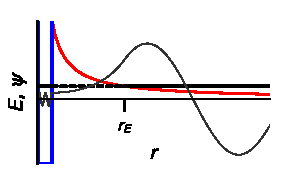
\includegraphics[width=\linewidth]{tunnel-schematic}
\caption{Tunneling through the Coulomb potential barrier. Not to scale.}
\label{f.tunneling}
\end{marginfigure}

\begin{exercisebox}[Turning radius for proton-proton collision in solar plasma]
\label{ex.turning-radius}
For the sun, typical center-of-mass energies are $E \sim \val{1}{\keV}$ (horizontal black line in Fig.~\ref{f.tunneling}). Suppose we have two protons heading towards one another with this kinetic  energy. What is their distance of closest approach?
\end{exercisebox}

As shown in Exercise~\ref{ex.turning-radius}, the turning radius $r_{E}$ at typical stellar energies is much larger than the nuclear radius.  Classically the particle can't penetrate the region $r_{n} < r < r_{E}$ where $E < V$ (dotted black line, Fig.~\ref{f.tunneling}); under classical physics, there would be no nuclear reactions at typical stellar temperatures because two particles would never find themselves close enough to be bound by the nuclear force.

The world is quantum, however, and the uncertainty in a particle's position means there is a small probability for the nucleons to be close enough for the nuclear force to come into play. In the classically forbidden region $r_{n} < r < r_{E}$, the particle wavefunction (thin gray line, Fig.~\ref{f.tunneling}) decreases exponentially, so that the probability to reach $r\sim\val{1}{\fermi}$ is
\[ \mathcal{P}\approx \exp\left[-2\pi^{2}\frac{r_{E}}{\lambda}\right] \]
where $\lambda = h/p$, $p$ being the momentum of the particle.
It is convenient to rewrite the argument of the exponential in terms of the particle energy,
\[ \frac{2\pi^{2}r_{E}}{\lambda} = 2\pi^{2}\left(\frac{Z_{1}Z_{2}e^{2}}{E}\right)
	\left(\frac{p}{h}\right) = \left[\pi \frac{Z_{1}Z_{2}e^{2}\sqrt{2m}}{\hbar}\right]\left(\frac{1}{E}\right)^{1/2}, \]
so that the probability of ``tunneling'' through the Coulomb barrier is
\begin{equation}
\mathcal{P} \approx \exp\left[-\left(\frac{\EG}{E}\right)^{1/2}\right],
\end{equation}
with
\[ \EG \equiv \textrm{``Gamow Energy''} = \left[\frac{2\pi^{2}Z_{1}^{2}Z_{2}^{2}e^{4}m}{\hbar^{2}}\right] = Z_{1}^{2}Z_{2}^{2}A \times \val{979}{\keV}.
\]
Our reaction cross-section is therefore the nuclear cross-section multiplied by the probability of tunneling, 
\begin{equation}\label{e.s-def}
\sigma(E) = \frac{S(E)}{E}\exp\left[-\left(\frac{\EG}{E}\right)\right].
\end{equation}
For many reactions $S(E)$ is nearly constant over the range of typical energies in a stellar plasma; this is helpful, as the reaction cross-section can be measured in the lab at higher energies and then extrapolated to the much lower stellar energies.

\newthought{To get the reaction rate from the cross-section,} recall that the mean-free path of a particle is $\ell = (n\sigma)^{-1}$, where $n$ is the density of targets. For definiteness, let us consider a particle of type 1. The mean-free path of this particle against reactions with particles of type 2 is therefore $\ell = (n_{2}\sigma)^{-1}$. If the particles are traveling with relative speed $v = |\bvec{v}_{1}-\bvec{v}_{2}|$, then the mean time between collisions is $\ell/v$. Thus in a large ensemble of particles, the mean rate of reactions is
\[
	r_{12} = \frac{n_{1} v}{\ell} = n_{2}n_{1}\langle\sigma v\rangle.
\]
Here $\langle \sigma v\rangle$ is the mean value of $\sigma v$ for all pairs of particles in the plasma.
For reactions between particles of the same type, we replace $n_{1}n_{2}$ with $n^{2}/2$; the factor of $1/2$ is to avoid double-counting.

A detailed calculation of the thermally averaged cross-section $\langle\sigma v\rangle$ is presented in Box~\ref{sb.thermally-averaged-cross-section}; here we'll just give a brief physical explanation for its value. There are two competing terms. First, the cross-section has an exponential term $\exp[-(\EG/E)^{1/2}]$ that increases rapidly with energy: more energetic particles have a much higher probability of tunneling through the Coulomb barrier. On the other hand, however, in a plasma the number of particles with energy $E$ decreases as $\exp(-E/\kB T)$.

As a result, reactions predominately occur in a narrow window of energies \Epk\ about a sort of geometric mean between \EG\ and $\kB T$:
\[	\Epk = \frac{\EG^{1/3}(\kB T)^{2/3}}{4^{1/3}}. \]
The reaction rate is suppressed for $E\ll\Epk$ because the probability of penetrating the Coulomb barrier is so small; the reaction rate is suppressed for $E\gg\Epk$ because there simply aren't enough particles with the relevant center-of-mass energy.

\begin{sidebar}[The thermally averaged cross section]
\label{sb.thermally-averaged-cross-section}
Since the cross-section depends on energy, the rate at which any given particle of type 1, traveling with velocity $\bvec{v}_{1}$, will react with particles of type 2 having velocities $\bvec{v}_{2}$ in a range $\dif^{3}v_{2}$ is
\[ n_{2} \sigma |\bvec{v}_{1}-\bvec{v}_{2}| \left(\frac{m_{2}}{2\pi \kB T}\right)^{3/2}\exp\left(-\frac{m_{2}v_{2}^{2}}{2\kB T}\right) \,\dif^{3}v_{2}. \]
The extra terms are because the particles have a Maxwell-Boltzmann distribution of velocities. To get the total rate per unit volume, we then have to multiply by the number of particles of type 1 having velocities $\bvec{v}_{1}$ in a range $\dif^{3} v_{1}$ and integrate over $\dif^{3}v_{1}\,\dif^{3}v_{2}$:
\begin{eqnarray}\label{e.rate-joint}
\lefteqn{r_{12} = n_{1}n_{2}  \left[\frac{m_{1}m_{2}}{(2\pi \kB T)^{2}}\right]^{3/2}}
  \nonumber\\ &&\times\int\! \sigma(E) v\exp\left(-\frac{m_{1}v_{1}^{2}}{2\kB T}-\frac{m_{2}v_{2}^{2}}{2\kB T}\right)  \,\dif^{3} v_{1}\,\dif^{3}v_{2}.
\end{eqnarray}
Now $E$ and $v$ are the relative energies and velocity in the center-of-mass frame.  We can change variable using the relations
\begin{eqnarray*}
\bvec{v}_{1} &=& \bvec{V} - \frac{m_{2}}{m_{1}+m_{2}} \bvec{v}\\
\bvec{v}_{2} &=& \bvec{V} + \frac{m_{1}}{m_{1}+m_{2}} \bvec{v}.
\end{eqnarray*}
where $V$ is the center-of-mass velocity. It is straightforward to show that $\dif v_{1,x}\,\dif v_{2,x} = \dif V_{x}\dif v_{x}$, and likewise for the $y,z$ directions.  Furthermore, $m_{1}v_{1}^{2} + m_{2}v_{2}^{2} = (m_{1}+m_{2})V^{2} + m v^{2}$, and multiplying and dividing the integral in equation~(\ref{e.rate-joint}) by $m_{1}+m_{2}$ allows us to write
\begin{eqnarray*}
\lefteqn{r_{12} = n_{1}n_{2} \left(\frac{m_{1}+m_{2}}{2\kB T}\right)^{3/2}\left(\frac{m}{2\kB T}\right)^{3/2}}\\
&&\times \int\!\dif^{3}V \int\!\dif^{3}v \,\sigma(E)v \exp\left[-\frac{mv^{2}}{2\kB T}\right]
 \exp\left[-\frac{(m_{1}+m_{2})V^{2}}{2\kB T}\right].
\end{eqnarray*}
The integral over $\dif^{3}V$ can be factored out and is normalized to unity. Hence we have for the reaction rate between a pair of particles 1 and 2, 
\begin{eqnarray}\label{e.rate}
r_{12} &=& n_{1}n_{2}\left\{\left(\frac{m}{2\pi\kB T}\right)^{3/2}\int_{0}^{\infty}\! \sigma(E) v \exp\left(-\frac{mv^{2}}{2\kB T}\right)  4\pi v^{2}\,\dif v\right\}.\nonumber\\
 &\equiv& n_{1}n_{2}\langle\sigma v\rangle.
\end{eqnarray}
The term in $\{\}$ is the averaging over the joint distribution of the cross-section times the velocity, and is usually denoted as $\langle\sigma v\rangle$. Note that if particles 1 and 2 were identical, then we would need to divide $r_{12}$ by 2.

Changing variables to $E = mv^{2}/2$ in equation~(\ref{e.rate}) and inserting the formula for the cross-section, equation~(\ref{e.s-def}), gives
\begin{equation}\label{e.integral}
\langle\sigma v\rangle = \left(\frac{8}{\pi m}\right)^{1/2}\left(\frac{1}{\kB T}\right)^{3/2}\int_{0}^{\infty}\!S(E)\exp\left[-\left(\frac{\EG}{E}\right)^{1/2}-\frac{E}{\kB T}\right]\,\dif E.
\end{equation}
Now, we've assumed that $S(E)$ varies slowly; but look at the argument of the exponential. This is a competition between a rapidly rising term $\exp[-(\EG/E)^{1/2}]$ and a rapidly falling term $\exp(-E/\kB T)$. As a result, the exponential will have a strong peak, and we can expand the integrand in a Taylor series about the maximum. Let 
\[
f(E) = -\left(\frac{\EG}{E}\right)^{1/2} - \frac{E}{\kB T}.
\]
Then we can write 
\begin{eqnarray*}
\lefteqn{\int_{0}^{\infty}\!S(E)\exp\left[-\left(\frac{\EG}{E}\right)^{1/2}-\frac{E}{\kB T}\right]\,\dif E}\\
&\approx&
	\int_{0}^{\infty}\! S(\Epk)\exp\left[f(\Epk) + \frac{1}{2}\left.\frac{\dif^{2} f}{\dif E^{2}}\right|_{E=\Epk}\left(E-\Epk\right)^{2}\right]\,\dif E.
\end{eqnarray*}
Here $\Epk$ is found by solving $(\dif f/\dif E)|_{E=\Epk} = 0$. By expanding the argument of the exponential, we have approximated the integrand by a Gaussian,
\[
	\exp\left[-\frac{(E-\Epk)^{2}}{2\varsigma^{2}}\right]
\]
where
\[
	\frac{1}{\varsigma^{2}} = -\left.\frac{\dif^{2} f}{\dif E^{2}}\right|_{E=\Epk}.
\]
This trick of approximately a steeply peaked function as a Gaussian, is known as the \newterm{method of steepest descent}.

Solving for \Epk, we get
\[
\Epk = \frac{\EG^{1/3}(\kB T)^{2/3}}{2^{2/3}},
\]
and 
\[ \exp\left[f(\Epk)\right] = \exp\left[-3\left(\frac{\EG}{4\kB T}\right)^{1/3}\right].
\]
Further,
\[
\left.\frac{1}{2}\frac{\dif^{2}f}{\dif E^{2}}\right|_{E=\Epk} = -\frac{3}{2(2\EG)^{1/3}(\kB T)^{5/3}} = -\frac{3}{4\Epk \kB T}.
\]
Defining a variable $\Delta = 4(\Epk \kB T/3)^{1/2}$, our integral becomes
\begin{eqnarray}\label{e.integral2}
\lefteqn{\langle\sigma v\rangle = \left(\frac{8}{\pi m}\right)^{1/2}\left(\frac{1}{\kB T}\right)^{3/2} S(\Epk)} \nonumber\\
&&\times 
  \exp\left[-3\left(\frac{\EG}{4\kB T}\right)^{1/3}\right]\int_{0}^{\infty}\!\exp\left[-\frac{(E-\Epk)^{2}}{(\Delta/2)^{2}}\right]\,\dif E.
\end{eqnarray}
%How well does this approximation do?  Figure~\ref{f.integrand} shows the integrand (\emph{solid line}) and the approximation by a Gaussian (\emph{dashed line}).  Although the integrand is skewed to the right, the area is approximately the same.
Another simplification can be made because both the Gaussian and the original integrand go to zero as $E\to 0$.  As a result, we can extend the lower bound of our integral (eq.~[\ref{e.integral2}]) to $-\infty$, and obtain
\begin{eqnarray}\label{e.rate2}
\langle\sigma v\rangle &\approx& \left(\frac{8}{\pi m}\right)^{1/2}\left(\frac{1}{\kB T}\right)^{3/2} S(\Epk) \exp\left[-3\left(\frac{\EG}{4\kB T}\right)^{1/3}\right]\frac{\Delta}{2}\nonumber\\
 &=& \frac{2^{13/6}}{\sqrt{3m}}\frac{\EG^{1/6}}{(\kB T)^{2/3}} \exp\left[-3\left(\frac{\EG}{4\kB T}\right)^{1/3}\right]  S(\Epk).
\end{eqnarray}
\end{sidebar}

%\begin{marginfigure}
%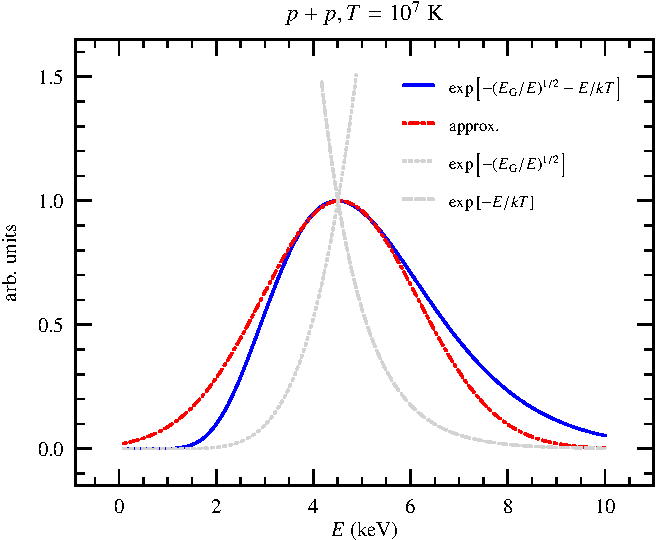
\includegraphics[width=\linewidth]{coulomb_integrand}
%\caption[Terms in integrand for calculating Coulomb barrier]{Integrand of eq.~(\protect\ref{e.integral}) (\emph{solid line}) and the Gaussian (\emph{dot-dashed line}) constructed by expanding to second order the argument of the exponential. The parameters for $\EG$ were taken from the $p+p$ reactions ($Z_{1}Z_{2}=1$, $A = 1/2$), and the temperature is $\val{10^{7}}{\K}$.  Note that the grey curves, showing the two terms of the exponential, have been rescaled to fit on the same plot.}
%\label{f.integrand}
%\end{marginfigure}

Using this approximation the rate can be evaluated, with $\langle\sigma v\rangle$ being given by eq.~(\ref{e.rate2}).
At stellar energies, reaction rates are incredibly sensitive to temperature. To quantify this, approximate the rate at a given temperature as a power-law, $r(T)\propto T^{n}$. Then the exponent is
\begin{equation}\label{e.exponent}
 n(T) = \dd{\ln r}{\ln T} = -\frac{2}{3} + \left(\frac{\EG}{4\kB T}\right)^{1/3},
\end{equation}
as you can verify for yourself (Exercise~\ref{ex.power-law}). On to some numbers. Table~\ref{t.reaction} lists quantities for some common reactions. 
In the table, the exponent $n(T)$ is evaluated at $T = \val{10^{7}}{\K}$. Note the large value of $n(T)$ at stellar temperatures. 
 
\begin{table}[hb]
\caption{\label{t.reaction} Parameters for non-resonant reactions}
\begin{tabular}{lrrrrrr}
 & $\pt+\pt$ & $\pt+\helium[3]$ & $\helium[3]+\helium[3]$ & $\pt+\lithium[7]$ & $\pt+\carbon$\\
\hline
%$A$ & 1/2 & 3/4 & 3/2 & 0.88 & 0.92 \\
%$Z_{1}Z_{2}$ & 1 & 2 & 4 & 3 & 6 \\
$\EG$ (MeV) & 0.489 & $2.94$ & $23.5$ & $7.70$ & $32.5$\\
%$\EG/(4k)$ (GK) & $1.4$ & $8.5$ & $68.0$ & $22.0$ & $94.0$ \\
$\Epk|_{T=\val{10^{7}}{\K}}$ (keV) & 4.5 & 8.2 & 16.3 & 11.3 & 18.2\\
%$\Delta/\Epk|_{T=\val{10^{7}}{\K}}$ & 1.0 & 0.75 & 0.53 & 0.64 & 0.50 \\
$n(T = \val{10^{7}}{\K})$ & 4.6 & 8.8 & 18.3 & 12.4 & 20.5\\
\end{tabular}
\end{table}

\begin{exercisebox}[Approximating a function as a power-law]
\label{ex.power-law}
Suppose we wish to approximate a function $f(x)$ at a point $x_{0}$ with a power-law, $p(x;A,n) = Ax^{n}$. Impose the condition $p(x_{0};A,n) = f(x_{0})$ and $\dif p/\dif x |_{x=x_{0}} = \dif f/\dif x|_{x=x_{0}}$ to find the parameters $A$ and $n$, and show that
\[
	n = \DD{\ln f}{\ln x}.
\]
Apply this to the reaction rate, eq.~(\ref{e.rate2}), and thus derive eq.~(\ref{e.exponent}).
\end{exercisebox}

\section{Hydrogen burning}

\subsection{Hydrogen burning via pp reactions: the lower main sequence}

In a contracting pre-main sequence star, the reaction $\hydrogen[2]+p\to\gamma+\helium[3]$ proceeds rapidly owing to the small Coulomb barrier; in fact, this reaction can occur in objects as small as $\approx \val{12}{M_{\mathrm{Jupiter}}}$.  The small primordial abundance of deuterium, however, prevents this reaction from doing anything more than slowing contraction slightly.  The reaction $\pt +\pt$ is much slower, because there is no bound nucleus \helium[2]; the only possible way to form a nucleus is to have a weak interaction as well, giving the reaction $\pt+\pt\to e^{+}+\nu_{e}+\hydrogen[2]$.

The weak cross section goes roughly as $\sigma_{\mathrm{weak}} \sim \val{10^{-20}}{\barn}\left(E/\keV\right)$, so that
\[ \frac{\sigma_{\mathrm{weak}}}{\sigma_{\mathrm{nuc}}} \sim 10^{-23}\left(\frac{E}{\keV}\right). \]
The $S$-factor for the $\pt+\pt$ reaction is very small, and as a result the characteristic temperature for this reaction to occur is $\approx \val{\sci{1.5}{7}}{\K}$; at this temperature, the lifetime of a proton to forming deuterium via capture of another proton is about $\val{6}{\Giga\yr}$.  Once a deuterium nucleus is formed, it is immediately destroyed via $\hydrogen[2]+p\to\gamma+\helium[3]$. The nucleus \lithium[4] is unbound with a lifetime of $\val{10^{-22}}{\second}$; the nucleus \beryllium[6] is likewise unbound ($\tau \sim \val{\sci{5}{-21}}{\second}$). As a result, the next reaction that can occur is $\helium[3]+\helium[3]\to 2\pt+\helium$.  Despite having a much greater Gamow energy than $\pt + \pt$, this reaction still is much faster than $\pt+\pt$ owing to the small weak cross-section.

In addition to capturing another \helium[3], it is also possible that
\begin{eqnarray}
\helium[3] + \helium &\to& \beryllium[7] + \gamma\nonumber\\
 \beryllium[7] + e^{-} &\to& \lithium[7] +  \nu_{e}\qquad(\tau=\val{53}{\unitstyle{d}})\nonumber \\
 \lithium[7] + \pt &\to& 2\helium + \gamma;
 \end{eqnarray}
furthermore, at slightly higher temperatures \beryllium[7] can capture a proton instead of an electron, giving the third branch
\begin{eqnarray}
\beryllium[7] + \pt &\to& \boron[8] + \gamma\nonumber\\
\boron[8] &\to& \beryllium[8] + e^{+} + \nu_{e}\qquad(\tau = \val{770}{\milli\second})\nonumber\\
\beryllium[8] &\to& 2\helium\qquad(\tau= \val{10^{-16}}{\second}).
\end{eqnarray}
 The end result of these chains is the conversion of hydrogen to helium, although the amount of energy carried away by neutrinos differs from one chain to the next.

\subsection[The CNO cycle]{Hydrogen burning via the CNO cycle: the upper main sequence}

As we saw in the previous section, the smallness of the $\pt+\pt$ cross-section means that captures onto heavier nuclei can be competitive at stellar temperatures.  Let's get a rough estimate of how charged a nucleus can be before the Coulomb barrier makes the reaction slower than $\pt+\pt$.  Assuming $A = 2Z$, and taking the $S$-factor for $\pt+\pt$ to be $10^{-22}$ times smaller that that for $\pt + \mathrm{^{A}Z}$ gives us the rough equation
\[ 10^{-22}\exp\left(-\frac{33.81}{T_{6}^{1/3}}\right) \approx \exp\left(-\frac{41.47 Z^{2/3}}{T_{6}^{1/3}}\right), \]
where the factors in the exponentials come from the peak energy for the reaction (see the handout on nuclear burning), and $T_{6}\equiv (T/\val{10^{6}}{\K})$.  Solving for $Z$, we see that at $T_{6} = 10$, proton captures onto \carbon\ have a comparable cross-section to $\pt + \pt$; at $T_{6} = 20$, proton captures onto \oxygen\ have a comparable cross-section.

Thus at temperatures slightly greater than that in the solar center, the following catalytic cycle becomes possible.
\begin{center}
\begin{tabular}{rr}
reaction & $\log[(\tau/\yr) \times (\rho X_{H}/\val{100}{\grampercc})]$\\
\hline
$\carbon(\mathbf{p},\gamma)\nitrogen[13]$ & 3.82\\
$\nitrogen[13](,e^{+}\nu_{e})\carbon[13]$ & $\tau=\val{870}{\second}$\\
$\carbon[13](\mathbf{p},\gamma)\nitrogen[14]$ & 3.21\\
$\nitrogen[14](\mathbf{p},\gamma)\oxygen[15]$ & 5.89 \\
$\oxygen[15](,e^{+}\nu_{e})\nitrogen[15]$ & $\tau = \val{178}{\second}$\\
$\nitrogen[15](\mathbf{p},\mathbf{^4He})\carbon$ & 1.50 \\
\hline
\end{tabular}
\end{center}
As indicated by the boldfaced symbols, this cycle takes in 4 protons and releases 1 helium nucleus.
The reaction timescales are evaluated at a temperature of $\val{20}{\Mega\K}$.
The reaction $\nitrogen+\pt\to\gamma+\oxygen[15]$ is by far the slowest step in the cycle; as a result, all of the CNO elements are quickly converted into \nitrogen\ in the stellar core, and this reaction controls the rate of heating.  At $T = \val{\sci{2}{7}}{\K}$, $\dif \ln \varepsilon_{\mathrm{CNO}}/\dif\ln T = 18$; in contrast the $\pt+\pt$ reaction has a temperature exponent of only 4.5.

The strong temperature dependence of the CNO burning has two effects on the structure of the star.  First, it makes the central temperature nearly constant over a wide range of stellar masses for $M > \val{1}{\Msun}$. A constant central temperature implies, via the virial theorem, that $R \propto M$ on the upper main sequence.  A second consequence is that nearly all of the star's luminosity is generated in a small mass about the stellar center.  This drives the cores of massive stars to be convective.



\chapter{The Main Sequence}\label{ch.main-sequence}
% !TEX root = ../intro-stellar-physics.tex

We now have almost all of the physics necessary to describe the structure of a star. We only need two additional items: we must consider whether the fluid is at rest or whether there is circulation, and we must discuss how the equation of state deviates from that of a classical ideal gas at high densities. These changes in the equation of state are important for low-mass stars and set the minimum stellar mass.

\section{Convection}\label{s.convection}

We've established that in the interior of the star a temperature gradient,
\[
	\DD{T}{r} = -\frac{3\rho\kappa_{R}}{4acT^3}\frac{L(r)}{4\pi r^2},
\]
arises to transport heat outward (cf.\ eq.~[\ref{e.gradient-temperature}]).
This gradient becomes steeper as we increases either the flux $L/4\pi r^{2}$ or the mean opacity $\kappa_{\mathrm{R}}$. There is a limit, however, to the magnitude of $|\dif T/\dif r|$: if the gradient is too steep, the warm fluid becomes buoyant relative to the cooler fluid above it and begins to rise. You are familiar with this phenomenon: picture a hot summer day. As the ground absorbs sunlight, it warms the air just above the ground. The warm air rises and forms updrafts. You have perhaps seen hawks circling as they are carried aloft by these updrafts. This circulation of fluid induced by a temperature gradient is known as \newterm{convection}. 

You can do a home demonstration of convection.  Brew tea, and pour the hot tea into a saucepan that is on an unlit burner. Use a straw to inject a layer of cold milk under the warm tea in the saucepan. The temperature difference between the tea and milk will inhibit their mixing. Light the burner, and watch for the development of convection---you will know it when you see it (Fig.~\ref{f.tea}).

\begin{figure}[htbp]
\forceversofloat
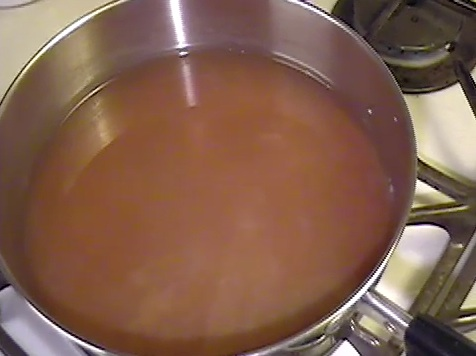
\includegraphics[width=0.5\linewidth]{convection-1}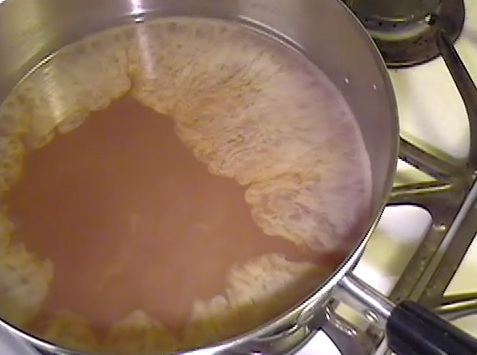
\includegraphics[width=0.5\linewidth]{convection-2}
\caption[Onset of convection]{Onset of convection in a tea-milk mixture.\label{f.tea}}
\end{figure}

Convection can also occur in stars, in regions of high flux and/or high opacity. During convection, the fluid velocities in question are typically quite subsonic, so hydrostatic equilibrium abides. But the fluid motions do make an enormous difference to heat transport! Warm fluid is carried upward and cool fluid sinks. The net result is that heat is transported upward much faster than it would have been if only diffusion had been operating. This upward transport of heat modifies the temperature gradient. In this chapter, we shall derive the condition for the onset of convection, and the value of the temperature gradient in the presence of subsonic, efficient convection.

\subsection{The onset of convection}\label{s.convection-onset}

To understand when convection starts, it helps to recall why a parcel of warm air rises. Recall Archimedes' law:
\begin{quote}\itshape
The buoyant force on an object, either wholly or partially immersed in a fluid under a constant gravitational acceleration, equals the weight of the fluid it displaces.
\end{quote}
What does this mean? A boat of mass $m$ displaces (pushes aside) a volume $v$ of water (density $\rho_{\mathrm{w}}$ when floating. The weight of this displaced water, $\rho_{\mathrm{w}}v g$, must equal the weight of the boat $mg$, so that $v = m/\rho_{\mathrm{w}}$.

\begin{exercisebox}[A boat with a weight]
Suppose we have a toy boat carrying a weight and floating in a tank as shown in the top panel of Fig.~\ref{f.archimedes}. The depth of the water in the tank is $d$. The weight is then removed from the boat and allowed to sink to the bottom of the tank (bottom panel, Fig.~\ref{f.archimedes}). Does the depth of water in the tank increase, decrease, or stay the same? Explain your reasoning.
\end{exercisebox}
\begin{marginfigure}[-6\baselineskip]
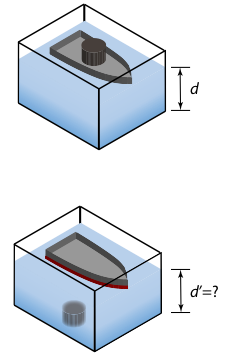
\includegraphics[width=\linewidth]{archimedes}
\caption[A boat with a weight]{\label{f.archimedes} A boat with a weight in a tank.}
\end{marginfigure}

We can use Archimedes' law---which is just an application of hydrostatic equilibrium---to determine whether a fluid in planar geometry and hydrostatic equilibrium,
\begin{equation}
\frac{\dif P}{\dif r} = -\rho g,
\end{equation}
and with a temperature gradient is unstable to convection. Imagine moving a blob of fluid upwards from $r$ to $r+h$.  We raise the blob slowly enough that it is in hydrostatic equilibrium with its new surroundings,\sidenote{We'll use the subscript $b$ to denote properties of the blob; quantities without a subscript refer to the background fluid.} $P_{b}(r+h) = P(r+h)$. We do move the blob quickly enough, however, that it doesn't exchange heat with its surroundings and therefore doesn't remain in \emph{thermal} equilibrium with its new environment. 

As a result of this lack of heat exchange, the upward motion of the blob is \newterm{adiabatic}.  \marginnote{Recall that pressure equilibrium in the blob is established over the time a sound wave takes to cross the blob. Thus, moving the blob slowly enough to maintain pressure equilibrium means that the motion is quite subsonic. Moving the blob quickly enough to prevent heat transport means (cf.\ exercise~\ref{ex.random-walk-diffusion}) that the blob is much larger than a mean free path so the time for photons to random walk across the blob is longer than time taken to raise the blob.}
To understand what this means, recall the first law of thermodynamics, which relates the change in internal energy $\dif U$ and in volume $\dif V$ to the heat transferred $\dif Q = T\,\dif S$:
\begin{equation}\label{e.first-law-thermo}
	\dif Q = T\,\dif S = \dif U + P\,\dif V,
\end{equation}
where $P$ is the pressure, $T$ the temperature, and $S$ the entropy. During an adiabatic process, $\dif Q = T\,\dif S = 0$. The entropy of the blob is therefore constant, 
$S_{b}(r+h) = S_{b}(r) = S(r)$, and is therefore not equal, in general, to the entropy of the surrounding gas at $r+h$: $S_{b}(r+h)  \neq S(r+h)$. The pressure in the blob, however, is the same as in the surrounding gas: $P_{b}(r+h) = P(r+h)$.

As in our discussion of the equation of state (cf.\ eq.~[\ref{e.ideal-gas-eos}]), it isn't really convenient to write things in terms of volume. To put eq.~(\ref{e.first-law-thermo}) into a more convenient form, divide both sides by the mass of the blob $m_{b}$:
\begin{eqnarray}
	\dif\left(\frac{Q}{m}\right) = T\,\dif\left(\frac{S}{m}\right) &=&
		\dif\left(\frac{U}{m}\right) + P\,\dif\left(\frac{V}{m}\right)\nonumber\\
	T\,\dif s &=& \dif u + P\,\dif\left(\frac{1}{\rho}\right)\nonumber\\
	T\,\dif s &=& \dif u - \frac{P}{\rho^{2}}\dif\rho \label{e.specific-first-law-thermo}
\end{eqnarray}
Here we denote the \emph{entropy per mass} and the \emph{energy per mass} by $s$ and $u$ respectively; and we identify the volume per mass with $1/\rho$, where $\rho$ is the mass density. Equation~(\ref{e.specific-first-law-thermo}) is the first law of thermodynamics as written for fluid dynamics.

After the blob has moved from $r$ to $r+h$, it has expanded so that its density is
\[
	\rho_{b}(r+h) = \rho[P_{b}(r+h),s_{b}(r+h)] = \rho[P(r+h),s(r)].
\]
Here we've written the density as a function of pressure and entropy: $\rho(P,s)$. Now we can apply Archimedes' law: if the density of the blob is greater than that of the surrounding fluid, then the buoyant force will be less than the weight of the blob; as a consequence, the blob will sink back to its original location. The fluid is thus stable. In contrast, if the density of the blob is less than that of the surrounding fluid, then the buoyant force is greater than the weight of the blob; a result, the fluid is unstable, as a small perturbation leads to the acceleration of the blob upwards. Figure~\ref{f.convective-schematic} has a schematic of this criterion.
\begin{marginfigure}[-6\baselineskip]
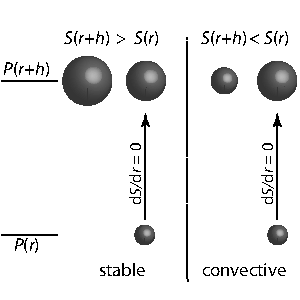
\includegraphics[width=\textwidth]{convective}
\caption[Illustration of criteria for convective instability]{\label{f.convective-schematic}Illustration of criteria for convective instability.  On the left, raising a blob a distance $h$ adiabatically and in pressure balance with its surrounding results in a higher density $V_{b} < V$, or $\rho_{b} > \rho$.  This is stable: the blob will sink back.  On the right, the blob is less dense and hence buoyant: it will continue to rise.}
\end{marginfigure}

Thus, for the fluid to be stable, we require that the density of the displaced blob be greater than that of the surrounding fluid:
\begin{eqnarray}
\rho_{b}(r+h) &>& \rho(r+h) \nonumber\\
\rho[P(r+h),s(r)] &>& \rho[P(r+h),s(r+h)].
\label{e.archimedes}
\end{eqnarray}
If condition (\ref{e.archimedes}) is satisfied, then the blob will be restored to its original location after a perturbation, and the system is stable. If condition (\ref{e.archimedes}) is not satisfied, then the blob will continue to rise following a perturbation; the system is thus unstable.

Since $h$ is an infinitesimal displacement, we can expand the right-hand side of eq.~(\ref{e.archimedes}):
\[
	\rho[P(r+h),s(r+h)] \approx \rho[P(r+h),s(r)] + \tderiv{\rho}{s}{P}\DD{s}{r}\;h.
\]
Here the notation $(\partial \rho/\partial s)_{P}$ means taking the derivative of $\rho$ with respect to $s$ while holding $P$ fixed. The condition for stability is therefore, after canceling common factors,
\begin{equation}\label{e.convective-stability}
 \tderiv{\rho}{s}{P}\frac{\dif s}{\dif r}< 0 .
\end{equation}
We've dropped $h$ from the left-hand side since it is positive.
We can put eq.~(\ref{e.convective-stability}) into a more useful form by changing variables from entropy $\rho$ to temperature $T$ via
\[
\tderiv{\rho}{T}{P} = \tderiv{\rho}{s}{P}\tderiv{s}{T}{P} = \tderiv{\rho}{s}{P}\frac{C_{P}}{T},
\]
where we used the specific heat at constant pressure, $C_{P}\equiv T(\dif s/\dif T)_{P}$.
Inserting this expression into eq.~(\ref{e.convective-stability}) gives
\[
 \frac{T}{C_{P}}\tderiv{\rho}{T}{P}\frac{\dif s}{\dif r} < 0,
\]
Now, $(\partial \rho/\partial T)_{P}$ is negative (gas expands on being heated), while $C_{P}$ is positive; hence eq.~(\ref{e.convective-stability}) will be satisfied wherever
\begin{equation}\label{e.entropy-condition}
\frac{\dif s}{\dif r} > 0.
\end{equation}
\begin{quote}\itshape
In a convectively stable star, the entropy must increase with radius.
\end{quote}
If this condition is not satisfied, if $\dif s/\dif r < 0$, then convection occurs: high-entropy material is buoyant and moves outward, while lower-entropy material sinks and moves inward. Eventually the rising fluid will mix with the surrounding material; when it does, its entropy will be added to the surrounding material, thereby raising its entropy. As a result of this mixing, the entropy gradient will be driven toward the marginally stable configuration $\dif s/\dif r = 0$.

\subsection{The adiabatic thermal gradient}\label{s.adiabatic-gradient}

Condition (\ref{e.entropy-condition}) for convective stability is not directly useful, since our equations of stellar structure do not directly involve the entropy. We'd instead like to have the criterion for the onset of convection be expressed in terms of pressure and temperature, since those quantities appear in our stellar structure equations. To obtain such an equation, 
let's return to the first law expressed in terms of mass-specific quantities (eq.~[\ref{e.specific-first-law-thermo}]):
\[
	\dif q = T\,\dif s = \dif u -\frac{P}{\rho^{2}}\,\dif \rho.
\]
We can express the energy $u = u(\rho,T)$ as a function of temperature $T$ and density $\rho$. Then taking the differential gives
\[ \dif u = \tderiv{u}{T}{\rho}\dif T + \tderiv{u}{\rho}{T}\dif \rho, \]
and thus the first law can be written as
\[ \dif q = T\dif s = \tderiv{u}{T}{\rho}\dif T + \left[\tderiv{u}{\rho}{T} - \frac{P}{\rho^{2}}\right]\dif \rho. \]
Hence the heat needed to raise the temperature of one kilogram of fluid while holding density fixed is
\begin{equation}\label{e.CV}
C_{\rho} \equiv T\,\tderiv{s}{T}{\rho} = \tderiv{u}{T}{\rho}.
\end{equation}
For an ideal gas, $u = u(T)$ and $C_{\rho}$ is approximately constant; hence we may integrate equation~(\ref{e.CV}) to obtain $u = C_{\rho}T + \textrm{const}$.

In Eq.~(\ref{e.specific-first-law-thermo}), the last term is $-(P/\rho)\, (\dif\rho/\rho) = -(P/\rho)\,\dif\ln\rho$. This motivates the following trick: take the logarithm of the equation of state, $\ln (P) = \ln(\rho) + \ln (T) + \ln (\kB/\mu\mb)$, and then take the differential to obtain
\[ \frac{\dif P}{P} = \frac{\dif\rho}{\rho} + \frac{\dif T}{T}. \]
Now eliminate $\dif\rho/\rho$ in the equation
\[ T\,\dif s = C_{\rho}\dif T - \frac{P}{\rho}\frac{\dif\rho}{\rho} \]
to obtain an expression for the heat transferred as a function of temperature and pressure,
\begin{equation}\label{e.first-law-pressure-temperature}
T\,\dif s = \left[C_{\rho} + \frac{P}{\rho T}\right]\dif T - \frac{1}{\rho}\dif P
	 = \left[C_{\rho} + \frac{\kB}{\mu\mb}\right]\dif T - \frac{1}{\rho}\dif P.
\end{equation}
The heat needed to raise the temperature of a mass of fluid while holding pressure fixed is therefore
\begin{equation}\label{e.CP}
C_{P}\equiv T\,\tderiv{s}{T}{P} = C_{\rho} + \frac{\kB}{\mu\mb}.
\end{equation}
For a plasma of ions and electrons, $C_\rho = (3/2)\kB/(\mu\mb)$ and hence $C_P = (5/2)\kB/(\mu\mb)$.  The ratio of specific heats is
\begin{equation}\label{e.gamma}
    \gamma = \frac{C_P}{C_\rho} = \frac{5/2}{3/2} = \frac{5}{3}.
\end{equation}
This value of $\gamma$ is for an ideal gas and does not hold universally.

\newthought{During adiabatic motion, there is no heat exchange:} hence, the entropy is constant and we can write eq.~(\ref{e.first-law-pressure-temperature}) as
\begin{equation}\label{e.differential-entropy}
    T\dif s = \dif q = 0 = C_{P}\dif T - \frac{1}{\rho} \dif P.
\end{equation}
We replace $1/\rho$ using the ideal gas equation of state
to obtain
\begin{eqnarray}
     C_{P}\dif T &=& \frac{\kB}{\mu\mb}\frac{T}{P}\dif P \nonumber\\
     \frac{\dif T}{T} &=& \frac{C_{P}-C_{\rho}}{C_{P}} \frac{\dif P}{P}\nonumber\\
	&=& \frac{\gamma-1}{\gamma}\frac{\dif P}{P}.
\label{e.differential-adiabat}
\end{eqnarray}
Integrating both sides of the equation gives
\begin{equation}\label{e.adiabat}
 T = T_{0}\left(\frac{P}{P_{0}}\right)^{(\gamma-1)/\gamma},
\end{equation}
where $T_{0}$ and $P_{0}$ are the temperature and pressure at the beginning of the adiabatic process. Equation~(\ref{e.adiabat}) tells us how the temperature changes with pressure along an adiabat for an ideal gas\sidenote{We used a similar relation in determining the sound speed (Box~\ref{b.sound-speed}).}. Using the ideal gas equation of state we can convert eq.~(\ref{e.adiabat}) into a relation between temperature and density or between density and pressure along an adiabat.

\begin{exercisebox}[Adiabatic relations]
Use equations~(\ref{e.adiabat}) and (\ref{e.eos}) to derive a relation between temperature and density, and a relation between density and pressure, along an adiabat.
\end{exercisebox}

\begin{exercisebox}[Onset of convection]
The figure shows some hypothetical runs of temperature with respect to pressure in a gas in hydrostatic equilibrium.  Indicate which of these situations is convectively unstable, and explain why. Draw on that plot the pressure-temperature relation that would ensue once convection sets in.

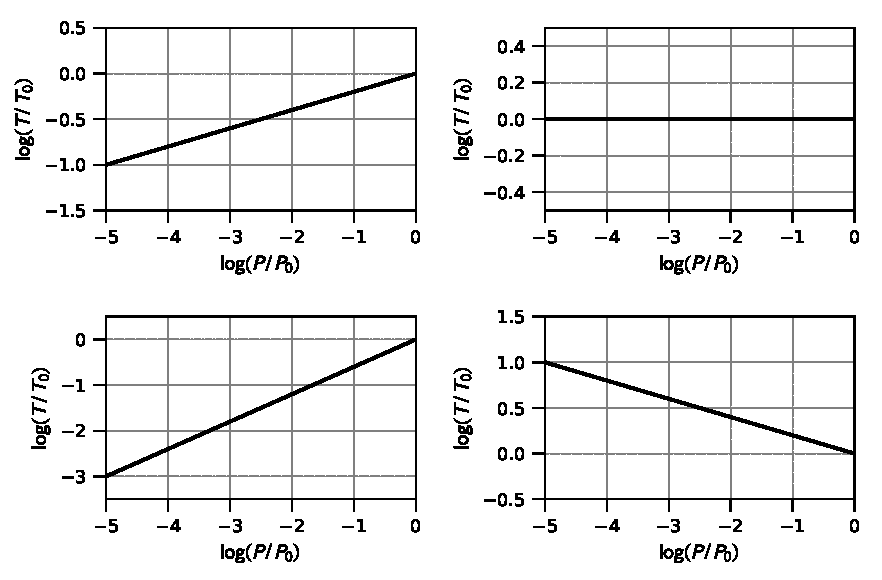
\includegraphics[width=\linewidth]{convection-worksheet-1}
\end{exercisebox}

\section{Convection in stars}
\label{s.convection-in-stars}

When convection is absent, the temperature gradient in the star is (eq.~[\ref{e.gradient-temperature}])
\[
    \DD{T}{r} = -\frac{3\rho\kappa}{4acT^3}\frac{L(r)}{4\pi r^2}.
\]
Here $\kappa$ is the opacity and $L(r)$ is the luminosity at radius $r$: $L/4\pi r^2$ is the flux. If this thermal gradient, $|\dif T/\dif r|$, becomes too large, however, the fluid becomes unstable: warm fluid begins to rise while cold fluid sinks. Over a wide range of stellar conditions this mixing drives the entropy gradient in the convectively unstable region to $\dif s/\dif r = 0$. The sun has a convective region just below its photosphere, Fig.~\ref{f.solar-convection}.
\begin{marginfigure}
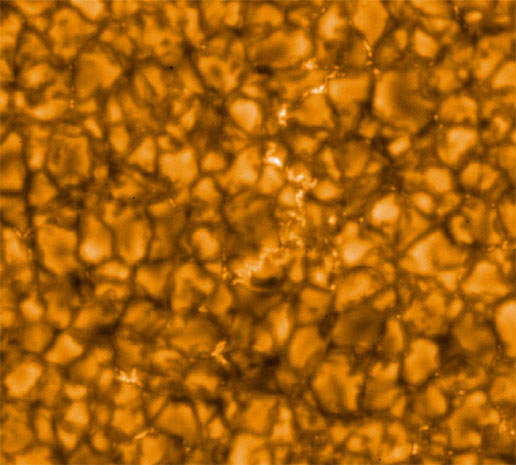
\includegraphics[width=\linewidth]{convection_hinode}
\caption[Solar convection cells]{\label{f.solar-convection} Solar convection cells, imaged with the Hinode Solar Optical Telescope. Image credit: Hinode JAXA/NASA/PPARC.}
\end{marginfigure}

We can recast Equation~(\ref{e.differential-adiabat}) as
\begin{equation}
    \frac{P}{T}\left(\dd{T}{P}\right)_s = \left(\dd{\ln T}{\ln P}\right)_s = \frac{\gamma-1}{\gamma}.
\label{e.nabla-adiabat}
\end{equation}
Hence, in a convective region,
\begin{eqnarray}
\DD{T}{r} &=& \frac{T}{P}\tderiv{\ln T}{\ln P}{s}\;\DD{P}{r} \nonumber\\
 &=& \frac{\gamma-1}{\gamma} \frac{T}{P}\; \DD{P}{r}.
\end{eqnarray}
The last form is specific to the case of an ideal gas.

\begin{exercisebox}[Temperature and density within a star]
The figure below indicates the central density and temperature (\emph{triangle}) for 3 hypothetical stars: (\emph{left}) a star that is fully convective; (\emph{center}) a star with a radiative (i.e., stable against convection) core (densities greater than $\val{10}{\kilo\gram\usk\meter^{-3}}$) and a convective envelope; (\emph{right}) a star with a convective core and a radiative envelope. For each star, sketch a plausible run of temperature with density within the star. In the center and right panels, the boundary between radiative and convective regions is marked with a vertical solid line.

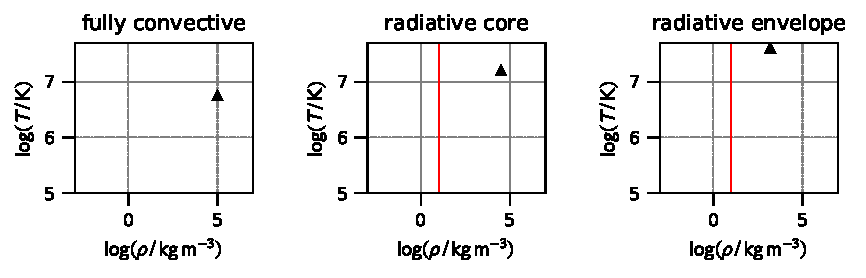
\includegraphics[width=\linewidth]{convection-worksheet-2}
\end{exercisebox}

%This occurs for large $\kappa$ (outer layers of cool stars) or for a high $L(r)/m(r)$ (centers of luminous hot stars).  On the main-sequence, stars with $M \lesssim \Msun$ have convective outer layers; stars with $M \lesssim \val{0.3}{\Msun}$ are fully convective. Stars with $M\gtrsim\Msun$ have convective cores.
%

\newthought{We can now collect the equations describing the structure of a star in steady-state}. Previously, we established the relations for the enclosed mass,
\begin{equation}\label{e.mass}
\DD{m}{r} = 4\pi r^{2}\rho,
\end{equation}
and the pressure,
\begin{equation}\label{e.pressure}
\DD{P}{r} = -\rho\frac{Gm}{r^{2}}.
\end{equation}
To these we add the equations for the temperature,
\begin{eqnarray}\label{e.temperature-radiative}
\DD{T}{r} &=& - \frac{L}{4\pi r^{2}}\frac{3\rho\kappa}{4ac T^{3}}\quad\textrm{where radiative; and}\\
\label{e.temperature-convective}
\DD{T}{r} &=& \frac{T}{P}\tderiv{\ln T}{\ln P}{S}\DD{P}{r}\quad\textrm{where convective}.
\end{eqnarray}
We finally add the equation for the luminosity,
\begin{equation}
\label{e.luminosity}
\DD{L}{r} = 4\pi r^{2}\rho\varepsilon.
\end{equation}
Equations (\ref{e.mass})--(\ref{e.luminosity}), or equivalently (\ref{e.lagrange-r})--(\ref{e.lagrange-L}), are supplemented by an equation of state $P = P(\rho,T,\{X\})$, opacity $\kappa = \kappa(\rho,T,\{X\})$, and heating rate $\varepsilon=\varepsilon(\rho,T,\{X\})$. Here $\{X\}$ refers to the abundances of the various isotopes. Note that we've omitted equations for the change in composition ($\dif X/\dif t$) due to nuclear burning. We've also omitted terms containing $\dif r/\dif t$, which describe expansion or contraction, from these equations.

\begin{sidebar}[The equations of stellar structure in Lagrangian form]
\label{sb.lagrangian-equations}
In general, the equations (\ref{e.mass}), (\ref{e.pressure}), (\ref{e.temperature-radiative})-(\ref{e.temperature-convective}), and (\ref{e.luminosity}) must be solved numerically. In practice, the radius $r$ is not the most convenient variable to use as a coordinate. In one dimension, the mass in each shell remains distinct, so the enclosed mass
\[
	m(r) = \int_{0}^{r} 4\pi r^{2}\rho\,\dif r
\]
makes a useful coordinate. Using the enclosed mass as a coordinate is called a \newterm{Lagrangian} description of the star.  Upon changing variables from $r$ to $m$, the structure equations become
\begin{eqnarray}
\DD{r}{m} &=& \frac{1}{4\pi r^{2}\rho}\label{e.lagrange-r}\\
\DD{P}{m} &=& \DD{P}{r}\DD{r}{m} = -\frac{Gm}{4\pi r^{4}}\label{e.lagrange-P}\\
\DD{T}{m} &=& - \frac{3\kappa L}{64\pi^{2} r^{4} acT^{3}}\qquad \textrm{where radiative}\label{e.lagrange-T-radiative}\\
\DD{T}{m} &=& -\frac{T}{P}\tderiv{\ln T}{\ln P}{S}\frac{Gm}{4\pi r^{4}} \quad \textrm{where convective}\label{e.lagrange-T-convective}\\
\DD{L}{m} &=& \varepsilon.\label{e.lagrange-L}
\end{eqnarray}
\end{sidebar}

\section{Contraction to the main sequence}
\label{s.contraction-to-main-sequence}

Stars are formed when clouds of gas and dust fall out of pressure balance and become unstable to gravitational collapse. Often, the cloud fragments into a myriad of small collapsing regions, such as in the Soul Nebula pictured in Fig.~\ref{f.soul-nebula}. In the center of these dense knots, a core comes into hydrostatic equilibrium and grows in mass as matter continues to infall. Much of this process is obscured from view by the surrounding clouds of gas and dust.
\begin{marginfigure}
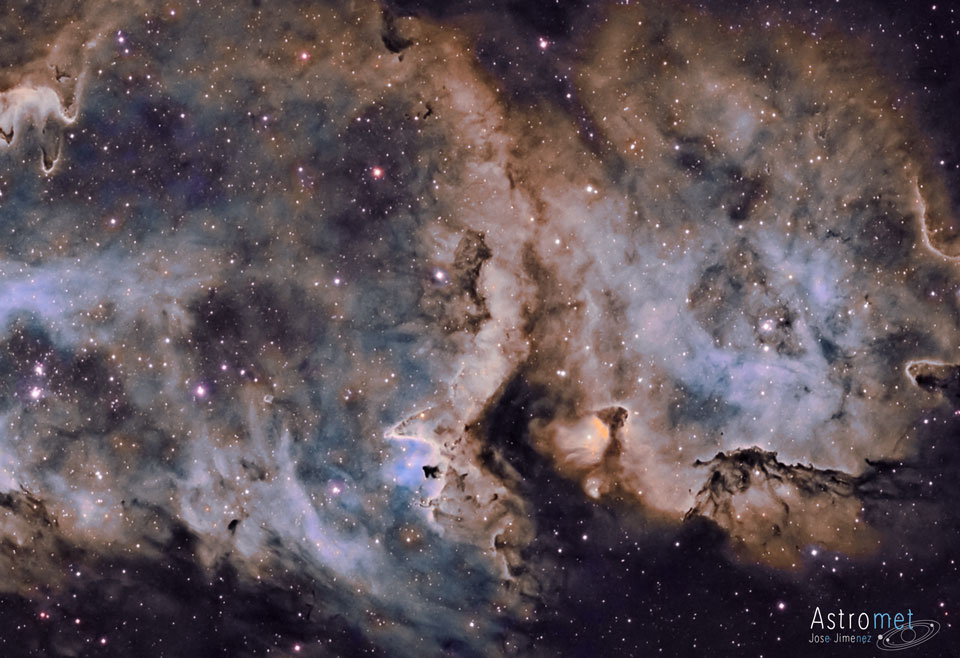
\includegraphics[width=\linewidth]{Soul_Priego_960}
\caption[Soul Nebula]{\label{f.soul-nebula} Image of the Soul Nebula (IC 1848) in the constellation Cassiopeia. Credit: Jos\'e Jim\'enez Priego (Astromet).}
\end{marginfigure}

As the nebula thins out, the star continues to contract slowly on a Kelvin-Helmholtz timescale, eq.~(\ref{e.kelvin-helmholtz}), as the core is still too cool for nuclear reactions to power the luminosity from the surface (remember, the luminosity is set by the mass of the star and its opacity). As the central temperature rises, the nuclear reaction rate increases rapidly until the heat released by reactions balances that emitted from the surface. At that point the star is on the \newterm{zero-age main sequence} (ZAMS). Of course, not all collapsing stellar-like objects reach the ZAMS---objects that are too low in mass will not ignite hydrogen fusion, while objects that are too high in mass tend to be unstable and eject mass. We'll explore these limits in the next few sections.

\begin{exercisebox}[Central temperature and density during contraction]
\label{ex.contraction-to-main-sequence}
This exercise revisits problem~\ref{ex.contraction-constant-density-protostar}. In that exercise you modeled how the density and temperature changed as a pre-main-sequence star contracted. Table~\ref{t.stellar-rhoT} gives central densities and temperatures of stars at the onset of hydrogen fusion (known as the \newterm{zero-age main sequence}). These temperatures and densities are plotted below and labeled by stellar mass. Assume an ideal-gas equation of state and use the virial relations for the temperature and central density to plot the tracks in this plane each star followed during its contraction.
\begin{center}
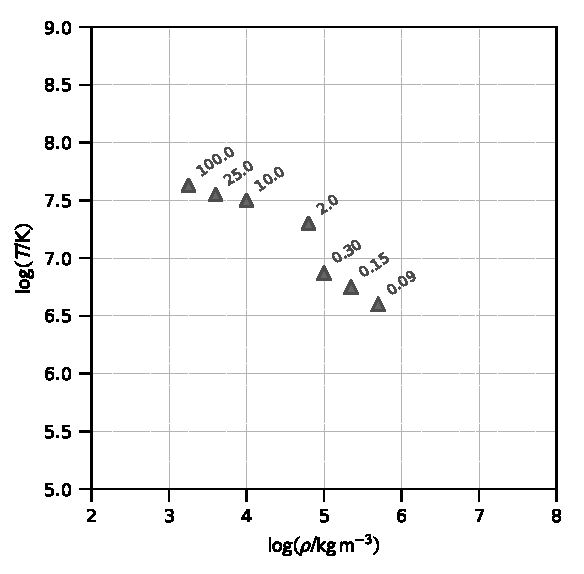
\includegraphics[width=0.8\linewidth]{rho-T-grid}
\end{center}
You will use this plot for exercises \ref{ex.minimum-stellar-mass} and \ref{ex.maximum-stellar-mass} as well.
\end{exercisebox}

\begin{margintable}[-16\baselineskip]
\caption[Central densities and temperatures of zero-age main-sequence stars]{\label{t.stellar-rhoT}Selected central densities and temperatures of zero-age main-sequence stars, computed with the \mesa\ stellar evolution code \citep{Paxton2010Modules-for-Exp}.}
\begin{tabular}{rrr}
$M/\Msun$ & $\log(\rho_{c}/\kilo\gram\,\meter^{-3})$ & $\log(T_{c}/K)$\\
\hline
0.09 & 5.70 & 6.60\\
0.15 & 5.35 & 6.75\\
0.30 & 5.00 & 6.87\\
2.0 & 4.80 & 7.30\\
10.0 & 4.00 & 7.50\\
25.0 & 3.60 & 7.55\\
100.0 & 3.25 & 7.63\\
\end{tabular}
\end{margintable}

\subsection{Degeneracy}
\label{s.degeneracy}

As a star contracts, the particles within it are packed ever closer together.  As we saw from our discussion of ionization, quantum mechanics enters the description of particle behavior when the separation between particles is of the order of the uncertainty in their positions.  Said differently, our classical description breaks down when the particle density exceeds roughly
\begin{equation}\label{e.heuristic-quantum-density}
    \frac{1\;\textrm{particle}}{(\Delta x)^3} 
    = \left(\frac{\Delta p}{h}\right)^3 
    \sim \left(\frac{m\kB T}{h^2}\right)^{3/2}.
\end{equation}
Another way to put this is that quantum effects become important when there is roughly 1 particle in a normalized phase space volume $\dif^{3}x\,\dif^{3}p/h^{3}$.

Suppose we have two identical particles in a quantum state. Since the particles are identical, if we exchange them the wavefunction can only change by a phase factor\sidenote{See Box~\ref{sb.identical-particles}} $e^{i\delta}$. If we exchange the particles again, we are back to our original state; as a result, $e^{2i\delta} = 1$, and therefore $\delta = 0$ or $\pi$. Hence upon the exchange of particles, the wavefunction either is unchanged ($\delta=0$) or it changes sign ($e^{i\pi}=-1$).
\begin{quote}\itshape
    There are two types of wavefunctions in this world: those that change sign under exchange; and those that don't.
\end{quote}
Particles that don't change sign under exchange are called \newterm{bosons} and have integer spin. Photons ($\textrm{spin} = 1$) are bosons. Particles that change sign under exchange are called \newterm{fermions} and have half-integer spin. Electrons, neutrinos, protons, and neutrons ($\textrm{spin} = 1/2$) are all fermions. 

A consequence of the fermion wavefunction changing sign when any two particles are exchanged is that the wavefunction vanishes if any two particles are in the same state---that is, they have the same position, momentum, and spin. For spin-half particles like electrons, this means we can put at most two such electrons in the same position and momentum state; we do this by having their spins antiparallel.

\begin{sidebar}[Identical particles]
\label{sb.identical-particles}
To understand how the interchange of identical particles works in more detail, let's start by recalling some features of quantum mechanics. This discussion is based on  \citet{Feynman1989The-Feynman-Lec}.
We denote a particle's state as $\ket{a}$, where $a$ is just a label.  For example, $a$ could be "electron with such-and-such momentum".  The probability of finding the electron in some other state $\ket{\phi}$ is given by $|\braket{\phi}{a}|^2$, where $\braket{\phi}{a}$ is a complex number known as the probability amplitude formed via an inner product of $\ket{\phi}$ and $\ket{a}$.

Now suppose we have two particles, a and b, and we scatter them so that one particle ends up in detector 1 and the other ends up in detector 2. There are two ways this can go, as shown here.
\begin{center}
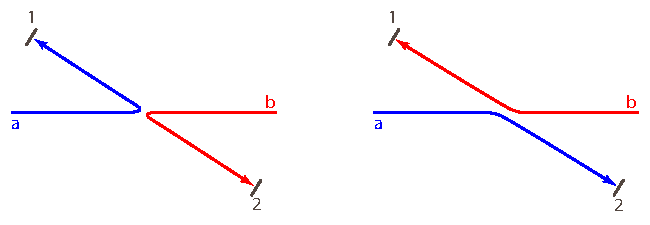
\includegraphics[width=\linewidth]{scattering-classical}
\end{center}
Classically, we would argue that the probability of getting either particle in detector 1 is just
\begin{equation}
    \mathcal{P}(\textrm{a or b in 1}) = \mathcal{P}(\textrm{a in 1}) + \mathcal{P}(\textrm{b in 1}).
\end{equation}
If particles a and b are different---e.g., one is a \carbon\ nucleus and the other is an \oxygen\ nucleus---then this holds in quantum mechanics as well. Quantum mechanically, we write
\begin{equation}
    \mathcal{P}(\textrm{a or b in 1}) = |\braket{1}{a}\braket{2}{b}|^2 + |\braket{2}{a}\braket{1}{b}|^2.
\end{equation}
If the particles are identical, however---for example, if a and b are two electrons with identical spin---then this picture is wrong.

Because of the uncertainty principle, we cannot follow the trajectories of a and b with infinite precision to see which is which; instead, the situation is more analogous to the depiction shown here.
\begin{center}
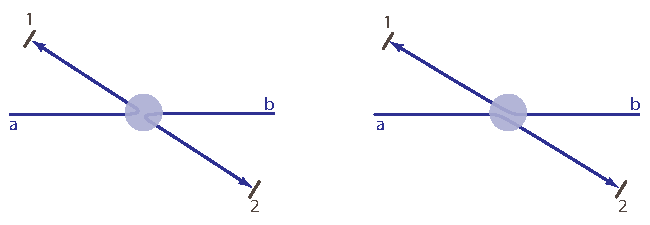
\includegraphics[width=\linewidth]{scattering-quantum}
\end{center}
There are now two indistinguishable ways of arriving at the final state---in this case, an electron in detector 1 and an electron in detector 2. According to quantum mechanics, we must therefore sum the amplitudes for getting to the final state, \emph{before taking the square}. That is, the probability for this one particle to end up in detector 1 and the other to end up in detector 2 is
\begin{eqnarray}
    \mathcal{P}(\textrm{a or b in 1}) &=& |\braket{1}{a}\braket{2}{b} + \braket{2}{a}\braket{1}{b}|^2\nonumber\\
    &=& |\braket{1}{a}\braket{2}{b}|^2 + |\braket{2}{a}\braket{1}{b}|^2 \nonumber\\
    && + {\color{red}\left[ \braket{1}{a}^*\braket{2}{b}^*\braket{2}{a}\braket{1}{b}\right.} \nonumber\\
    && {\color{red}+ \left.\braket{2}{a}^*\braket{1}{b}^*\braket{1}{a}\braket{2}{b}\right]} \nonumber\\
    &=& \mathcal{P}(\textrm{a in 1}) + \mathcal{P}(\textrm{b in 1}) \nonumber\\
    && + {\color{red}\left[ \braket{1}{a}^*\braket{2}{b}^*\braket{2}{a}\braket{1}{b}\right.}\nonumber\\
    && {\color{red}+ \left.\braket{2}{a}^*\braket{1}{b}^*\braket{1}{a}\braket{2}{b}\right]}.
    \label{e.scattering-quantum}
\end{eqnarray}
The probability of scattering an electron into detector 1 is the classical value plus the \emph{additional} interference term in $\color{red}[\cdot]$.

\newthought{To see the effect of this interference term on the thermal properties of the system,} let's imagine putting two particles into the same small volume.  To do this, we imagine the detectors 1 and 2 sliding together until they overlap, as shown here.  
\begin{center}
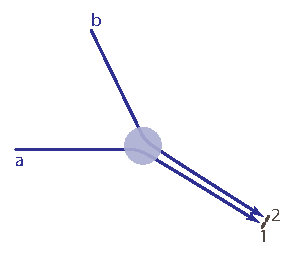
\includegraphics{fermions}
\end{center}
Since detectors 1 and 2 are approaching one another, we must have
\begin{equation}
    |\braket{1}{a}\braket{2}{b}|^2 = |\braket{2}{a}\braket{1}{b}|^2.
\end{equation}
This does not imply, however, that $\braket{1}{a}\braket{2}{b} = \braket{2}{a}\braket{1}{b}$: the amplitudes could differ by a phase factor, so that interchanging the particles would yield
\[
    \braket{2}{a}\braket{1}{b} = e^{i\delta}\braket{1}{a}\braket{2}{b}.
\]
If we interchange the particles, and then interchange them again, we get
\[
    \braket{1}{a}\braket{2}{b} = e^{2i\delta}\braket{1}{a}\braket{2}{b};
\]
since swapping the particles twice just gets up back to the original situation, we must have that $e^{2i\delta} = 1$ and therefore $e^{i\delta} = \pm 1$.

If there is no change of sign, i.e., $\braket{2}{a}\braket{1}{b} = \braket{1}{a}\braket{2}{b}$, then from equation~(\ref{e.scattering-quantum}) we have
\begin{equation}\label{e.boson}
    \mathcal{P}(\textrm{a or b in 1}) = 2|\braket{1}{a}\braket{2}{b}|^2 + 2|\braket{2}{a}\braket{1}{b}|^2.
\end{equation}
This is \emph{twice} the classical value: the probability of the particles entering the same state is enhanced.

In contrast, if the sign changes under exchange, i.e., if $\braket{2}{a}\braket{1}{b} = -\braket{1}{a}\braket{2}{b}$, then equation~(\ref{e.scattering-quantum}) implies that
\begin{eqnarray}
\mathcal{P}(\textrm{a or b in 1}) &=& |\braket{1}{a}\braket{2}{b}|^{2} + |\braket{2}{a}\braket{1}{b}|^{2} \nonumber\\ 
    && - |\braket{1}{a}\braket{2}{b}|^{2} - |\braket{2}{a}\braket{1}{b}|^{2} \nonumber\\ 
    &=& 0.\label{e.fermion}
\end{eqnarray}
\begin{quote}\itshape
We cannot have 2 identical particles with the same momentum, position, and spin if their wavefunction changes sign when the particles are exchanged.
\end{quote}
Particles with integer spin (i.e., their angular momentum is an integer multiple of $\hbar$) have wavefunctions that do not change sign under exchange; these particles are said to obey \newterm{Bose-Einstein statistics} and are called \newterm{bosons}.  Particles with half-integer spin have wavefunctions that do change sign under exchange; these particles are said to obey \newterm{Fermi-Dirac statistics} and are called \newterm{fermions}.  Photons are bosons; electrons, protons, neutrons, and neutrinos are fermions.
\end{sidebar}

\newthought{To account for Fermi-Dirac statistics within the equation of state,} we imagine a small volume containing $N$ electrons. Motivated by eq.~(\ref{e.heuristic-quantum-density}), we divide the phase space into cells,
\[
	\frac{\dif^{3}x\,\dif^{3}p}{h^{3}},
\]
and into each cell we place 2 electrons with opposing spins. We always add the electrons to the lowest open energy level, and repeat the process until we have added all $N$ electrons. This procedure is represented by the equation
\begin{equation}
\label{e.number-degenerate}
	N = \frac{2}{h^{3}}\int_{V}\dif^{3}x\int_{0}^{\EF}\dif^{3}p
\end{equation}
In this equation $\EF$, the \emph{Fermi energy}, is the energy of the last electron added and is the largest filled energy level.

If our volume is isotropic, then we can change variables: first, to spherical momentum coordinates, $\dif^{3}p = 4\pi p^{2}\,\dif p$; second, from $\dif p$ to $\dif\varepsilon$.  Since $p = \sqrt{2m\varepsilon}$, where $\varepsilon$ is the energy of a single electron,
\[
	\dif p = \sqrt{\frac{m}{2\varepsilon}}\,\dif \varepsilon;
\]
upon changing variables and integrating over $\varepsilon$ from $0$ to $\EF$ we obtain
\[
	N = \frac{8\pi}{h^{3}}V \int_{0}^{\EF} \sqrt{2}m^{3/2}\varepsilon^{1/2}\,\dif \varepsilon
	= \frac{8\pi}{3h^{3}} V (2m)^{3/2} \EF^{3/2}.
\]
Solving for the Fermi energy gives
\begin{equation}\label{e.fermi-energy}
	\EF = \frac{h^{2}}{2m}\left(\frac{3}{8\pi}\frac{N}{V}\right)^{2/3}.
\end{equation}
What is the total energy of our system? We again integrate over phase space, with each electron multiplied by its energy $\varepsilon$:
\begin{equation}\label{e.total-energy}
	E = \frac{8\pi}{h^{3}}V\int_{0}^{\EF}\sqrt{2}m^{3/2}\varepsilon^{3/2}\,\dif\varepsilon = \frac{8\pi}{5h^{3}}V(2m)^{3/2} \EF^{5/2}.
\end{equation}
Using eq.~(\ref{e.fermi-energy}) to substitute for $\EF$ in eq.~(\ref{e.total-energy}), we can find the energy per unit volume,
\[
	\frac{E}{V} = \frac{3}{5}\left(\frac{3}{8\pi}\right)^{2/3}\frac{h^{2}}{2m}n^{5/3} = \frac{3}{5} n \EF,
\]
where $n=N/V$ is the density of electrons.

For a non-relativistic gas the pressure is $P = (2/3)(E/V)$.  Hence the pressure of our electron gas is
\begin{equation}\label{e.pressure-electrons}
	P = \frac{2}{3}\frac{E}{V} = \frac{2}{5} n\EF
		= \frac{2}{5}\left(\frac{3}{8\pi}\right)^{2/3}\frac{h^{2}}{2m}n^{5/3}.
\end{equation}
Notice that the pressure is independent of the temperature.

Electrons, being more than 1000 times lighter than nuclei, become degenerate first. Suppose our composition consists of species with charge $Z_{i}$ and mass number $A_{i}$. Then the number of electrons per unit volume\sidenote{assuming complete ionization} is
\[
	n_{e} = \sum_{i} n_{i} Z_{i} = \frac{\rho}{\mb}\sum_{i} X_{i}\frac{Z_{i}}{A_{i}}.
\]
By analogy with the mean molecular weight, we define an electron mean weight
\begin{equation}\label{e.electron-mean-weight}
\mu_{e} \equiv \left(\sum_{i}X_{i}\frac{Z_{i}}{A_{i}}\right)^{-1}
\end{equation}
so that $n_{e} = \rho/(\mb\mu_{e})$.

\begin{exercisebox}[The mass-radius relation for a degenerate EOS]
\label{ex.degenerate-mass-radius}
Use equation~(\ref{e.electron-mean-weight}) in eq.~(\ref{e.pressure-electrons}) to express the pressure as a function of mass density $\rho$. The use the virial scalings for $P(M,R)$ and $\rho(M,R)$ to obtain a relation $R(M)$ for a degenerate object.
\end{exercisebox}

As you found in exercise~\ref{ex.degenerate-mass-radius}, when the star becomes degenerate, there is a unique radius for a given mass and composition. This is in contrast to the non-degenerate case, for which a star of a given mass can have a wide range of possible radii depending on the internal temperature.

Consider a contracting pre-main-sequence star. Initially, the star has a low density and the equation of state is that of an ideal non-degenerate gas. According to the virial theorem, as the radius decreases, both the central temperature and density increase. 
The radius decreases because the star is radiating away energy, and a star with an ideal, non-degenerate equation of state has a total energy that depends on its radius.

At some density, the equation of state will become degenerate. At this point, contraction comes to a halt. The star continues to radiate energy, but instead of contracting, the star simply cools while remaining at constant radius. If the contracting pre-main-sequence star is to become a main-sequence star, then, it must reach temperatures sufficient for hydrogen fusion to occur \emph{before} becoming degenerate.

\begin{exercisebox}[Minimum stellar mass]
\label{ex.minimum-stellar-mass}
The equation of state becomes degenerate roughly where $\kB T=\EF$, with $\EF$ begin given by eq.~(\ref{e.fermi-energy}). From this and eq.~(\ref{e.electron-mean-weight}), assuming a H-He composition with $X_{\mathrm{H}} = 0.7$ and $X_{\mathrm{He}}=0.3$, derive a relation between $\log(T)$ and $\log(\rho)$. Plot this relation on the phase diagram in exercise~\ref{ex.contraction-to-main-sequence}, and on the plot indicate which side of the relation is degenerate.
Given that contraction halts when the equation of state becomes degenerate, what does this plot imply for the minimum mass required to initiate hydrogen fusion?
\end{exercisebox}

\newthought{As shown in exercise \ref{ex.minimum-stellar-mass}, there is a minimum mass needed to initiate hydrogen fusion.} Contracting star-like objects of lower mass are known as \newterm{brown dwarfs}. Although dim, they are observable with spectral types ``L'', ``T'' or ``Y''\cite{Kirkpatrick1999Dwarfs-Cooler-t,Cushing2011The-Discovery-o}.

\begin{exercisebox}[Planetary masses and radii]
\label{ex.planetary-M-and-R}
You might notice that the degenerate mass-radius relation you found in exercise~\ref{ex.degenerate-mass-radius} can't hold for very light objects (or very heavy ones, for that matter). Earth, for example has a much larger mass than Mars, and also has a larger radius, contrary to what the degenerate relation predicts. What happens is that at low pressures, the Coulomb force comes into play---the atomic and molecular bonds that add variety to life. These bonds set the size and spacing of atoms, and therefore fix the density of matter. Let's model this. The typical size of an atom is the Bohr radius,
\[
	a_{\mathrm{B}} = \frac{4\pi\varepsilon_{0}\hbar^{2}}{m_{e}e^{2}} = \val{\sci{5.29}{-11}}{\meter}.
\]
	\begin{enumerate}
	\item Let take our mass density as being one average nuclear mass per volume $a_{\mathrm{B}}^{3}$.  We'll again use our solar composition, $X_{\mathrm{H}}=0.7, X_{\mathrm{He}}=0.3$.
What is the value of this density? Is it plausible?
	\item If matter is at this density, what is $R(M)$?
	\item Roughly for what mass object, if any, does this $R(M)$ relation intersect the relation for degenerate matter? This sets the mass at which degeneracy becomes important for a cold object. Compare this mass with objects in the solar system.
	\end{enumerate}
\end{exercisebox}

\subsection{Radiation pressure}
\label{s.radiation-pressure}

Radiation in thermal equilibrium exerts a pressure (eq.~\ref{e.radiation-pressure}): $\Prad = aT^{4}/3$. Because of this strong dependence on temperature, radiation pressure becomes an increasingly large fraction of the total pressure for massive stars. Stars that are radiation-pressure dominated tend to be unstable: they have strong winds and violent fits of mass ejection (see the image of Eta Carinae, Fig.~\ref{f.eta-carinae}). As a result, they lose copious amounts of mass while on the main sequence. This effectively sets a rough upper limit on the mass of a star.
\begin{marginfigure}[-12\baselineskip]
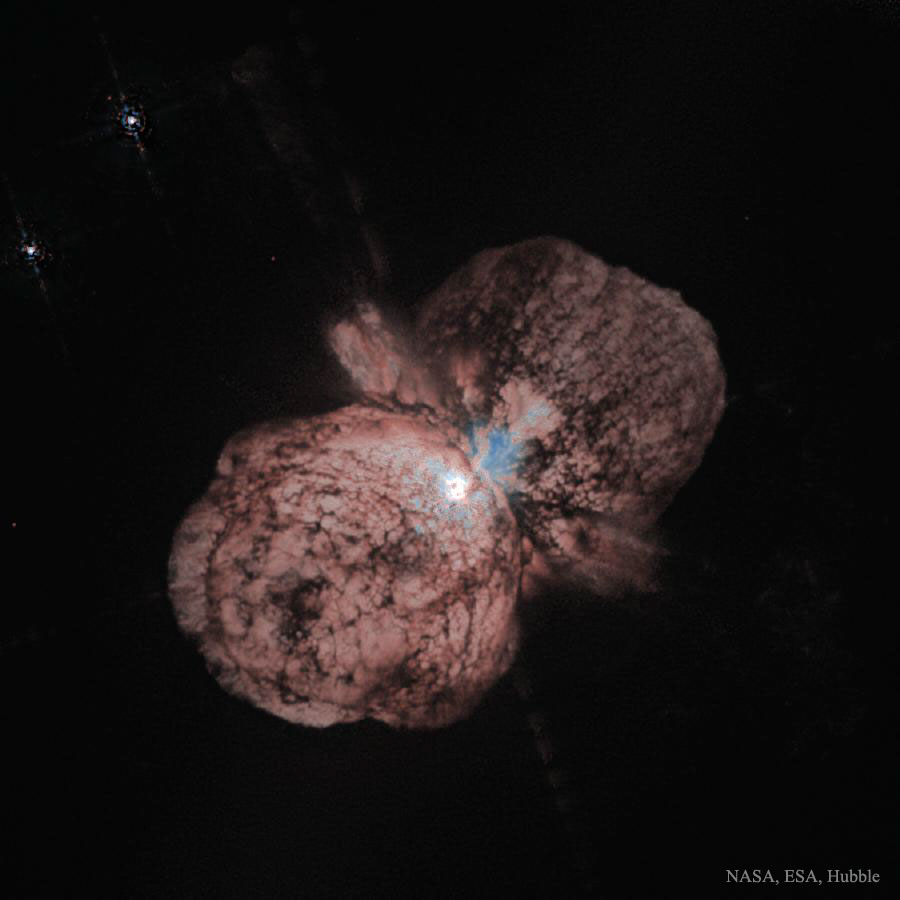
\includegraphics[width=\linewidth]{etacarinae_hubble_900}
\caption[Image of the massive star Eta Carinae]{\label{f.eta-carinae} Image of the massive star Eta Carinae. Credit: J. Morse (Arizona State U.), K. Davidson (U. Minnesota) et al., WFPC2, HST, NASA.}
\end{marginfigure}


\begin{exercisebox}[Radiation pressure]
Use the virial relations for density and temperature to estimate how the ratio $\Prad/P_{\!\mathrm{gas}}$ depends on the mass of the star.
\end{exercisebox}

\begin{exercisebox}[Maximum stellar mass]
\label{ex.maximum-stellar-mass}
The equation of state becomes dominated by radiation roughly where $P(\textrm{ideal gas}) \approx P(\textrm{radiation})$. Derive from this criterion a relation between $\log(T)$ and $\log(\rho)$, and plot this relation on the figure for exercise~\ref{ex.contraction-to-main-sequence}. Indicate which side of this relation is radiation-pressure dominated. What do your findings in this exercise imply for the mass range of main-sequence stars?
\end{exercisebox}

\section{Life on the main-sequence}

With the initiation of hydrogen fusion, the star settles into thermal and mechanical equilibrium, with its structure described by the solution of equations\sidenote{Or, in Lagrangian form, (\ref{e.lagrange-r})--(\ref{e.lagrange-L}).} (\ref{e.mass})--(\ref{e.luminosity}), along with the equation of state and prescriptions for the opacity $\kappa$ and heating rate $\varepsilon$. 

The reason for star's stability on the main sequence is a consequence of the relation, derived in exercise \ref{ex.gravithermal-specific-heat}, between the star's total energy and temperature. If the reaction rate were to increase and deposit more energy into the star, then since the total energy is $\propto -GM^{2}/R$, the star would expand. This expansion would cause the central temperature to decrease, thereby reducing the reaction rate.

The star is not in complete equilibrium, however, as hydrogen in the core is gradually being converted to helium. The timescale over which the composition changes is much longer than the dynamical timescale (sets hydrostatic equilibrium), the radiative diffusion timescale (sets thermal gradient), and the Kelvin-Helmholtz timescale (sets core temperature via growth or contraction of stellar radii). The gradual build-up of a helium-rich core does not, therefore, affect the stability of the star, but it does lead to a slow brightening of the star over its main sequence lifetime. For our sun, the gradual enrichment of the core in helium causes a slow increase in luminosity of $\approx10\%$ for each billion years.\marginnote{Although this slow increase in luminosity is not a drastic change, it has significant implications for life on Earth. The expected warming is sufficient to make Earth uninhabitable within about a billion years from now.} 

\begin{exercisebox}[Nuclear burning timescale]
\label{ex.nuclear-burning-timescale}
You computed in exercise \ref{ex.Q-hydrogen-helium} the energy released from the conversion of 4 hydrogen atoms into helium. Express this number in terms of the energy released per mass of hydrogen burned; this number should be in units of $\unitstyle{J}/\kilo\gram$. Now assume that the Sun's luminosity comes from the fusion of hydrogen into helium in the innermost 10\% of the Sun's mass. For a composition that is 70\% hydrogen by mass, how long would it take to deplete the hydrogen in the solar core? This sets the main-sequence lifetime of the sun.
\end{exercisebox}

The cool outer layers of low-mass stars have large opacities: for example many elements are not ionized, so there are many potential lines for absorption. As a result, stars with $M\lesssim\Msun$ have convective regions in their outer parts. The fraction of the star that is convective is larger for low-mass, cool stars; and stars with $M \lesssim\val{0.3}{\Msun}$ are fully convective, so that the whole interior lies along an adiabat. For more massive, hotter, stars, the opacities are lower, and as a result, the outer convective region vanishes for stars with $M\gtrsim\Msun$.

\begin{exercisebox}[Mass-luminosity relation]
\label{ex.mass-luminosity-relation}
We can estimate how the luminosity depends on stellar mass for stars that have a mostly radiative structure. Start with equation (\ref{e.temperature-radiative}) for the temperature gradient and approximate $\dif T/\dif r \approx T_{c}/R$, $\rho \approx \bar{\rho}$, $L/4\pi r^{2} \approx L/4\pi R^{2}$, and $T\approx T_{c}$. Take the opacity $\kappa$ to be constant,  use the virial estimate for the central temperature $T_{c}$ and express the mean density $\bar{\rho}$ in terms of stellar mass $M$ and radius $R$. After some algebra, you should find that the luminosity $L$ depends on $M$ to some power. Compare this scaling against the data in Table~\ref{t.stellar-properties}. Obtain an expression for the stellar lifetime as a function of mass, and calibrate it to the Sun's main-sequence lifetime, $\tau_{\odot}\sim\val{10}{\Giga\yr}$.
\end{exercisebox}

\newthought{Stars more massive than the Sun have sufficiently high core temperatures for hydrogen to be consumed via the CNO cycle.} The strong temperature dependence of the CNO burning has two effects on the structure of the star. First, it makes the central temperature nearly constant over a wide range of stellar masses for $M>\val{1}{\Msun}$---a small rise in temperature is sufficient to raise the heat production $\varepsilon$ to match the rise in luminosity. A nearly constant central temperature implies, via the virial theorem, that $R \propto M$ on the upper main sequence. The second consequence is that nearly all of the star's luminosity is generated in a small region about the stellar center. The flux, $L/4\pi r^{2}$, in this small region is enormous, and this makes the core of the star convective. The convection can mix hydrogen fuel into the core, which makes the lifetime somewhat longer than the estimate from exercise~\ref{ex.mass-luminosity-relation}. A summary of the structure of main sequence stars is contained in Table~\ref{t.MS-characteristics}.
\begin{margintable}
\caption{\label{t.MS-characteristics} Characteristics of main-sequence stars}
\centering
\begin{tabular}{lll}
 & $M\lesssim\Msun$ & $M\gtrsim\Msun$\\
\hline
$4\hydrogen\to\helium$ & pp & CNO\\
core is & radiative  & convective\\
envelope is & convective & radiative\\
\end{tabular}
\end{margintable}




\chapter{After the Main Sequence}\label{ch.post-main-sequence}
% !TEX root = ../intro-stellar-physics.tex

The depletion of hydrogen in the core heralds the end of the star's placid main-sequence life. We shall first give an overview of the changes that ensue. Fusion of helium requires a temperature $\gtrsim\val{10^{8}}{\K}$, substantially higher than that required for the fusion of hydrogen. As a result, when the hydrogen is used up helium burning cannot immediately begin, and the core contracts, similar to what happened before the star was born, with one crucial difference. As the helium core contracts, hydrogen continues to fuse in a shell surrounding the core. This shell burning intensifies as the core contracts and causes drastic changes to the star's radius, surface temperature, and luminosity.

Once the core becomes sufficiently hot, helium fuses into carbon, and the core again reaches a state of thermal and mechanical equilibrium. After a brief helium-burning phase, the core becomes depleted in helium and must again contract. As with pre-main sequence stars, the critical question is whether the core becomes degenerate before the next fusion reaction can ignite. For stars with main-sequence masses $\lesssim \valrng[--]{8}{10}{\Msun}$, the core becomes degenerate before the onset of $\carbon$ fusion, which requires temperatures $\approx\val{\sci{8}{8}}{\K}$.  Indeed, for stars around a solar mass, the fusion of \helium\ occurs under moderately degenerate conditions.\sidenote{Stars with masses $\lesssim\val{0.5}{\Msun}$ will become degenerate before reaching temperatures sufficient for helium to fuse; the main-sequence lifetime of such stars is much greater than the age of the universe, so making a helium white dwarf requires some kind of mass loss, such as in a binary.}
As a result, the cores of low-mass stars end up composed of carbon and oxygen (or perhaps oxygen and neon) and supported by degenerate electrons; such objects are known as \newterm{white dwarfs}.

For stars with masses $\gtrsim\valrng[--]{8}{10}{\Msun}$, the core is hot enough to avoid degeneracy until reactions in the core have made heavier isotopes up to \iron. At this point the matter reaches its maximum binding energy\sidenote{cf.\ exercise~\ref{ex.nuclear-landscape}}, so further heating from nuclear reactions is curtailed. A degenerate core forms and grows in mass due to reactions in shells surrounding the core. There is a maximum mass, known as the \newterm{Chandrasekhar mass}, that can be supported by electron degeneracy pressure. When the core exceeds this mass, it violently implodes. The implosion halts when matter reaches nuclear density and the repulsive strong nuclear force provides pressure support. In this implosion, most of the electrons and protons combine, $e^{-} + \pt \to \nt+\nu_{e}$. 
The resulting torrent of neutrinos injects energy into the outer layers of the star; in many cases this is sufficient to eject the outer layers of the star and produce a \newterm{supernova}. Left behind will be the core, now composed mostly of neutrons\sidenote{At densities substantially above that of an atomic nucleus other constituents, such as hyperons, may appear.} and known as a \newterm{neutron star}.

If the envelope is not ejected, matter will fall back onto the neutron star. The maximum mass that can be supported by the nuclear force is uncertain, but is somewhere between \valrng[--]{2}{3}{\Msun}; when this maximum mass is exceeded, the neutron star collapses into a black hole.
Having sketched the various end-of-life scenarios, we shall now explore them in more detail.

\section{Low-mass stars}

\subsection{Ascent of the red-giant branch}

With the depletion of hydrogen in the core, the core contracts. During this contraction, hydrogen fusion continues in a shell surrounding the core. The shell hydrogen fusion produces helium, which adds to the core mass. As the core contracts its temperature rises. The rising temperature and pressure at the base of the hydrogen-burning shell causes the reactions in the shell to go at an ever-increasing rate. The resulting increase in luminosity inflates the envelope, now fully convective, to large radii and hence to a low surface temperature: the star becomes a red giant. The high luminosity, combined with the low surface gravity of the distended envelope, drives a strong wind so that the star loses a substantial amount of mass during the giant phase.

\begin{marginfigure}
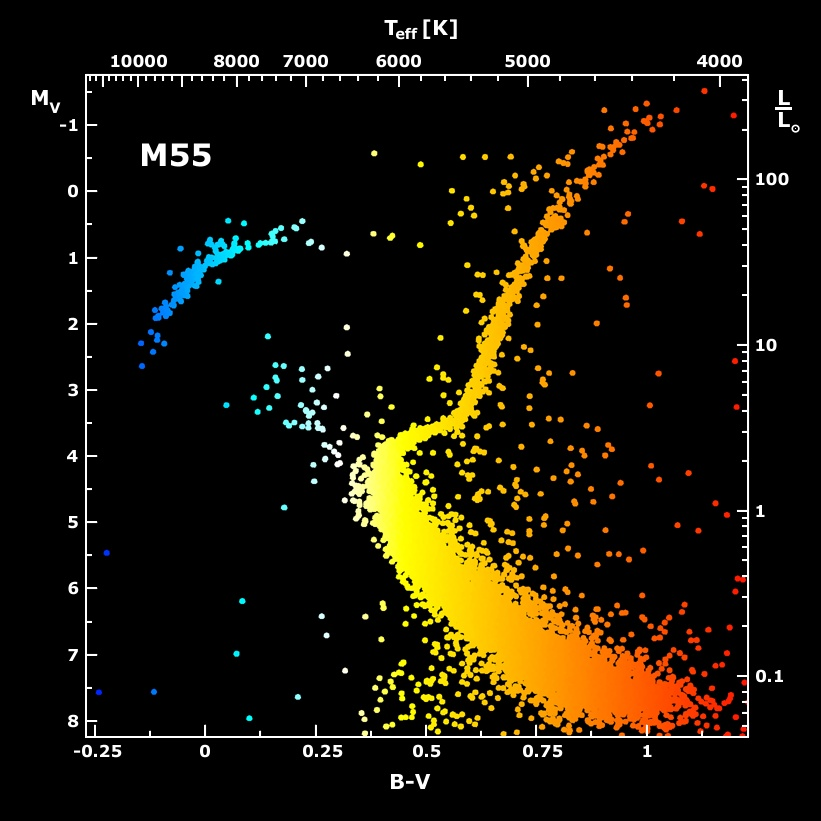
\includegraphics[width=\linewidth]{m55cmd_mochejska_big}
\caption[Color-magnitude diagram for the globular cluster M55]{\label{f.m55-cmd}Color-magnitude diagram for the globular cluster M55. \imgcred\ B.J. Mochejska, J. Kaluzny (CAMK), 1m Swope Telescope.}
\end{marginfigure}
Figure~\ref{f.m55-cmd} shows a color-magnitude diagram for the globular cluster M55. The figure plots the absolute $V$-band magnitude against the $(B-V)$ index---brighter and bluer stars at top left, dimmer and redder stars at lower right. The surface effective temperatures is indicated along the top axis, and the luminosity in solar units is indicated along the right axis.

Each dot on the plot represents a star, and the colors indicate how the star would appear. The main sequence forms a band running from the lower right to the center of the figure. At the time of the cluster's birth, the main-sequence would have continued on to the upper left of the plot.  Stellar mass increases as one moves upwards and leftwards along the main-sequance, and since more massive stars evolve faster, those bright, blue stars originally on the upper left of the main sequence have ended their hydrogen-burning tenure and moved on. From the location of the main-sequence turn-off, the age of the cluster is estimated\cite{VandenBerg2018Constraints-on-} to be $\val{12.9\pm0.8}{\Giga\yr}$. The red giant branch arcs from the center of the plot towards the upper right.  As stars turn away from the main sequence and their helium core mass grows, the stars move up the red giant branch becoming redder and more luminous.

\subsection{Helium burning: the horizontal branch}
There are no stable isotopes with mass number $A=5$ or $A=8$, which makes the fusion of \helium\ somewhat tricky. Although unstable, the isotope \beryllium[8] is relatively long-lived ($\val{10^{-16}}{\second}$) compared to a nuclear timescale\sidenote{Roughly the time for a pion to cross a nucleus, $\sim \val{10^{-22}}{\second}$.}. As a result,
when the core temperature reaches $\approx\val{10^{8}}{\K}$,\marginnote{The mass of a \beryllium[8] nucleus is $\val{91}{\kilo\eV}$ \emph{greater} than the mass of two \helium\ nuclei; at a temperature $\approx\val{10^{8}}{\K}$, the kinetic energy of the \helium\ nuclei is just enough to make up the difference.} the reaction
\[ \helium + \helium \longleftrightarrow\beryllium[8] \]
builds up a minute abundance of \beryllium[8]. This abundance is sufficient for the reaction
\[ \beryllium[8] + \helium \longleftrightarrow \carbon^{*} \]
to make a small abundance of \carbon\ in an excited state (denoted by the $^{*}$).  While most of the $\carbon^{*}$ decays back into $\beryllium[8]+\helium$, a small fraction decays instead to the ground state, $\carbon^{*}\to\carbon+\gamma$. The net result is $3\,\helium\to\carbon$, known as the \newterm{triple-alpha reaction}.

Once core \helium\ has ignited,\marginnote[-4\baselineskip]{The triple-alpha reaction is incredibly temperature-sensitive: $\partial\ln\epsilon_{3\alpha}/\partial\ln T \approx 40$ at $T = \val{10^{8}}{\K}$. This sensitivity, combined with the mildly degenerate conditions of the core, makes the ignition of \helium\ somewhat unstable for solar-mass stars.} the star settles onto a ``helium main sequence;'' observationally this is the \newterm{horizontal branch}, so called because these stars lie in a clump on a Hertzsprung-Russell diagram. The luminosity on the horizontal branch is about \valrng[--]{30}{100}{\Lsun}. The higher luminosity and the much lower energy release from the triple-alpha reaction make the horizontal branch lifetime much shorter than that of the main-sequence (e.g., the horizontal branch lifetime is $\sim \val{10^{8}}{\yr}$ for a solar-mass star). The horizontal branch is clearly visible as the blue arc in the upper-left quadrant of Fig.~\ref{f.m55-cmd}.

\begin{exercisebox}[Horizontal branch lifetime]
Use the result of exercise \ref{ex.energy-release} to find the heat released per kilogram from fusing 3 \helium\ nuclei into \carbon. Take the core mass to be $\val{0.45}{\Msun}$ (the minimum core mass needed for the ignition of helium), and find the lifetime for core helium burning for a horizontal branch luminosity of $\val{30}{\Lsun}$,.
\end{exercisebox}

\subsection{The asymptotic giant branch and emergence of a white dwarf}

As the mass of \carbon\ builds up in the core, the reaction $\carbon+\helium\to\oxygen$ begins to compete with the triple alpha reaction. As a result, the core becomes composed of a \carbon/\oxygen\ mixture.
With the depletion of \helium, the core---now composed of \carbon\ and \oxygen---again contracts, while the growing luminosity from the H- and He-burning shells again inflate the envelope to large radii. Observationally, this phase is the \newterm{asymptotic giant branch}: the stars move away from the horizontal branch and become redder and more luminous. This branch can be observed in Fig.~\ref{f.m55-cmd} arcing from the horizontal branch and asymptotically approaching the red giant branch at upper right. 

During the ascent of the asymptotic giant branch, the star's hydrogen-rich envelope is consumed at its base by the H- and He-burning shells and expelled at the surface by an increasingly strong wind. The expelled envelope resembles a nebula and is termed a \newterm{planetary nebula} (Fig.~\ref{f.NGC2392}). After the envelope has dispersed, the hot core---observed as a white dwarf---slowly cools. For a solar-mass star, the expected final mass of the core, and hence of the white dwarf, is $\approx\val{0.6}{\Msun}$.
\begin{marginfigure}
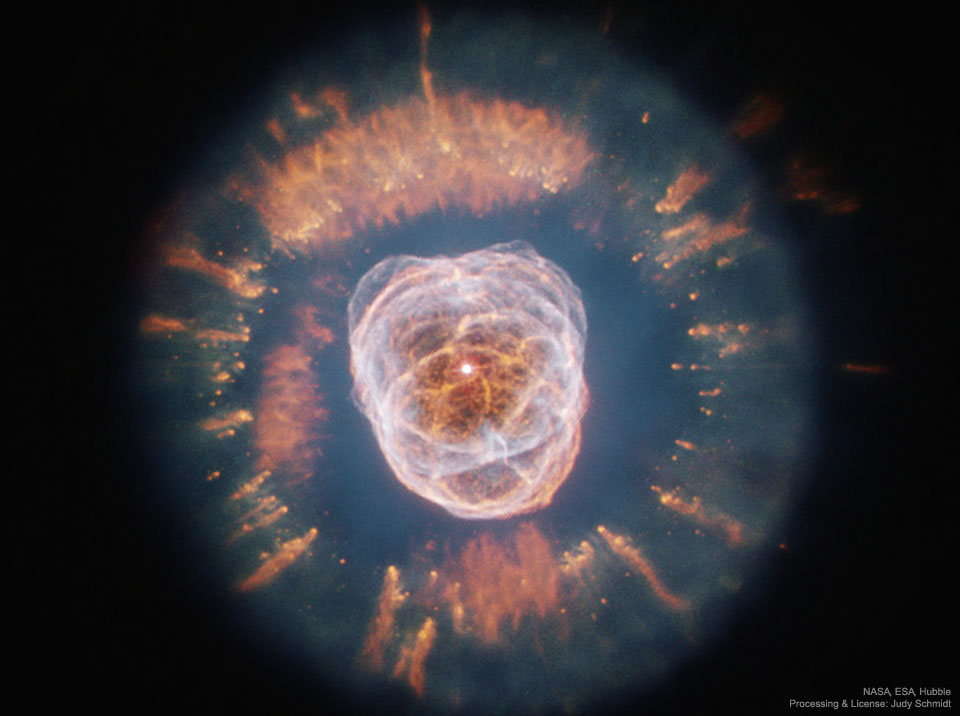
\includegraphics[width=\linewidth]{NGC2392_HubbleSchmidt_960}
\caption[The planetary nebula NGC 2392]{\label{f.NGC2392} The planetary nebula NGC~2392. \imgcred\ NASA, ESA, Hubble, Chandra; \emph{Processing \& \href{https://creativecommons.org/licenses/by/2.0/}{\ccby\ License}:} Judy Schmidt.}
\end{marginfigure}

\section{Massive stars}

For stars with main-sequence masses $\gtrsim \valrng[--]{8}{10}{\Msun}$, the fusion of \carbon\ commences while the core is non-degenerate and at a temperature $\approx\val{\sci{8}{8}}{\K}$.  At this temperature, electron-positron pairs form and annihilate ($e^{-}+e^{+}\longleftrightarrow\gamma\gamma$); occasionally instead of decaying into photons, the reaction
\[ e^{-}+e^{+} \longrightarrow \nu_{e} + \bar{\nu}_{e}\]
occurs instead and generates a neutrino-antineutrino pair. The mean free path for the neutrinos is larger than the radius of the star; as a result, the neutrinos stream out and take energy from the core. Because the neutrinos can easily leave the star, they end up carrying away the bulk of the heat from the core at these high core temperatures.

Within the core, \carbon\ is consumed by the reactions
\[ \carbon+\carbon\to\left\{\begin{array}{c}\sodium+\pt \\\neon+\helium\end{array}\right.. \]
The \pt\ and \helium\ capture onto other nuclei that are present.  At slightly higher temperatures, $\neon+\gamma \to \oxygen+\helium$ releases \helium\ nuclei that subsequently capture onto other \oxygen, \neon, and \magnesium. As the temperature increases, the next significant burning stage is
\[\oxygen+\oxygen\to\left\{\begin{array}{c}\phosphorus[31]+\pt \\ \silicon+\helium \end{array}\right. ;\]
as with $\carbon+\carbon$, the \pt\ and \helium\ combine with ambient nuclei with the end result being a distribution of isotopes about \silicon.

\begin{exercisebox}[Dynamical time of evolved stellar core]
At the onset of \oxygen\ burning in a \val{25}{\Msun} star, the central density (Table~\ref{t.burning-timescales}) is $\val{\sci{3.6}{9}}{\kilo\gram\,\meter^{-3}}$.  What is the dynamical time of the core?
\end{exercisebox}

The strong Coulomb barrier inhibits the fusion of nuclei beyond \oxygen; instead, photodissociation reactions such as $\silicon+\gamma \to \magnesium+\helium$ liberate \nt, \pt, and \helium.  These light nuclei then capture onto heavier nuclei, and the composition gradually becomes composed of isotopes about \iron.  This is \newterm{nuclear statistical equilibrium}: the composition is in the lowest energy state (most bound) for the ambient density and temperature. As a result, there is no further release of nuclear energy possible. The (mostly \iron) core contracts and becomes degenerate; its mass gradually increases from the burning of surrounding material.

The amount of energy available from the reactions with heavy nuclei is low; as a consequence, the time required for the core to deplete the available fuel grows shorter and shorter, with the final stages occurring in a day (column labeled $\tau$ in Table~\ref{t.burning-timescales}). After the ignition of carbon, the core evolves too quickly for the envelope to keep up. Thus the external appearance of the star provides no window into the final days of burning.

\begin{table}[htp]
\forcerectofloat\small
\caption[Nuclear burning timescales for massive stars]{\label{t.burning-timescales}Nuclear burning timescales for massive stars. Values taken from \citet{Woosley2002The-evolution-a}; neutrino luminosities are taken from \citet{Weaver1978Presupernova-ev} and do not exactly correspond to the same stellar models for the other parameters.}
\begin{tabular}{rrrrrr}
\multicolumn{5}{c}{hydrogen}\\
\hline
$M_{\mathrm{ZAMS}}$ & $T_{c}$ & $\rho_{c}$ & $L$ & $L_{\nu}$ & $\tau$\\
\Msun & $\val{10^{7}}{\K}$ & $\val{10^{3}}\kilo\gram\,\meter^{-3}$ & $\val{10^{3}}{\Lsun}$ & \Lsun & Myr\\
\hline
15 & 3.53 & 5.81 & 28 & --- &11.1\\
25 & 3.81 & 3.81 & 110 & --- & 6.7\\
\hline\hline
\multicolumn{5}{c}{helium}\\
\hline
$M_{\mathrm{ZAMS}}$ & $T_{c}$ & $\rho_{c}$ & $L$ & $L_{\nu}$ & $\tau$ \\
\Msun & $\val{10^{8}}{\K}$ & $\val{10^{6}}{\kilo\gram\,\meter^{-3}}$ & $\val{10^{3}}{\Lsun}$ & $\Lsun$ & Myr\\
\hline
15 & 1.78 & 1.39 & 41 & 1 &1.97\\
25 & 1.96 & 0.76 & 182 & 20 & 0.84\\
\hline\hline
\multicolumn{5}{c}{carbon}\\
\hline
$M_{\mathrm{ZAMS}}$ & $T_{c}$ & $\rho_{c}$ & $L$ & $L_{\nu}$ & $\tau$ \\
\Msun & $\val{10^{8}}{\K}$ & $\val{10^{9}}{\kilo\gram\,\meter^{-3}}$ & $\val{10^{3}}{\Lsun}$ & $\val{10^{3}}{\Lsun}$ & kyr \\
\hline
15 & 8.34 & 2.39 & 83 & 90 & 2.03\\
25 & 8.41 & 1.29 & 245 & 2600 & 0.52\\
\hline\hline
\multicolumn{5}{c}{oxygen}\\
\hline
$M_{\mathrm{ZAMS}}$ & $T_{c}$ & $\rho_{c}$ & $L$ & $L_{\nu}$ & $\tau$ \\
\Msun & $\val{10^{9}}{\K}$ & $\val{10^{9}}{\kilo\gram\,\meter^{-3}}$ & $\val{10^{3}}{\Lsun}$ & $\val{10^{6}}{\Lsun}$ & yr\\
\hline
15 & 1.94 & 6.66 & 87 & 2 & 2.58\\
25 & 2.09 & 3.60 & 246 & 6000 & 0.40\\
\hline\hline
\multicolumn{5}{c}{silicon}\\
\hline
$M_{\mathrm{ZAMS}}$ & $T_{c}$ & $\rho_{c}$ & $L$ & $L_{\nu}$ & $\tau$ \\
\Msun & $\val{10^{9}}{\K}$ & $\val{10^{10}}{\kilo\gram\,\meter^{-3}}$ & $\val{10^{3}}{\Lsun}$ & $\val{10^{6}}{\Lsun}$ & d\\
\hline
15 & 3.34 & 4.26 & 87 & $10^{5}$ & 18.3\\
25 & 3.65 & 3.01 & 246 & $10^{6}$ & 0.7\\
\end{tabular}
\end{table}

\begin{marginfigure}
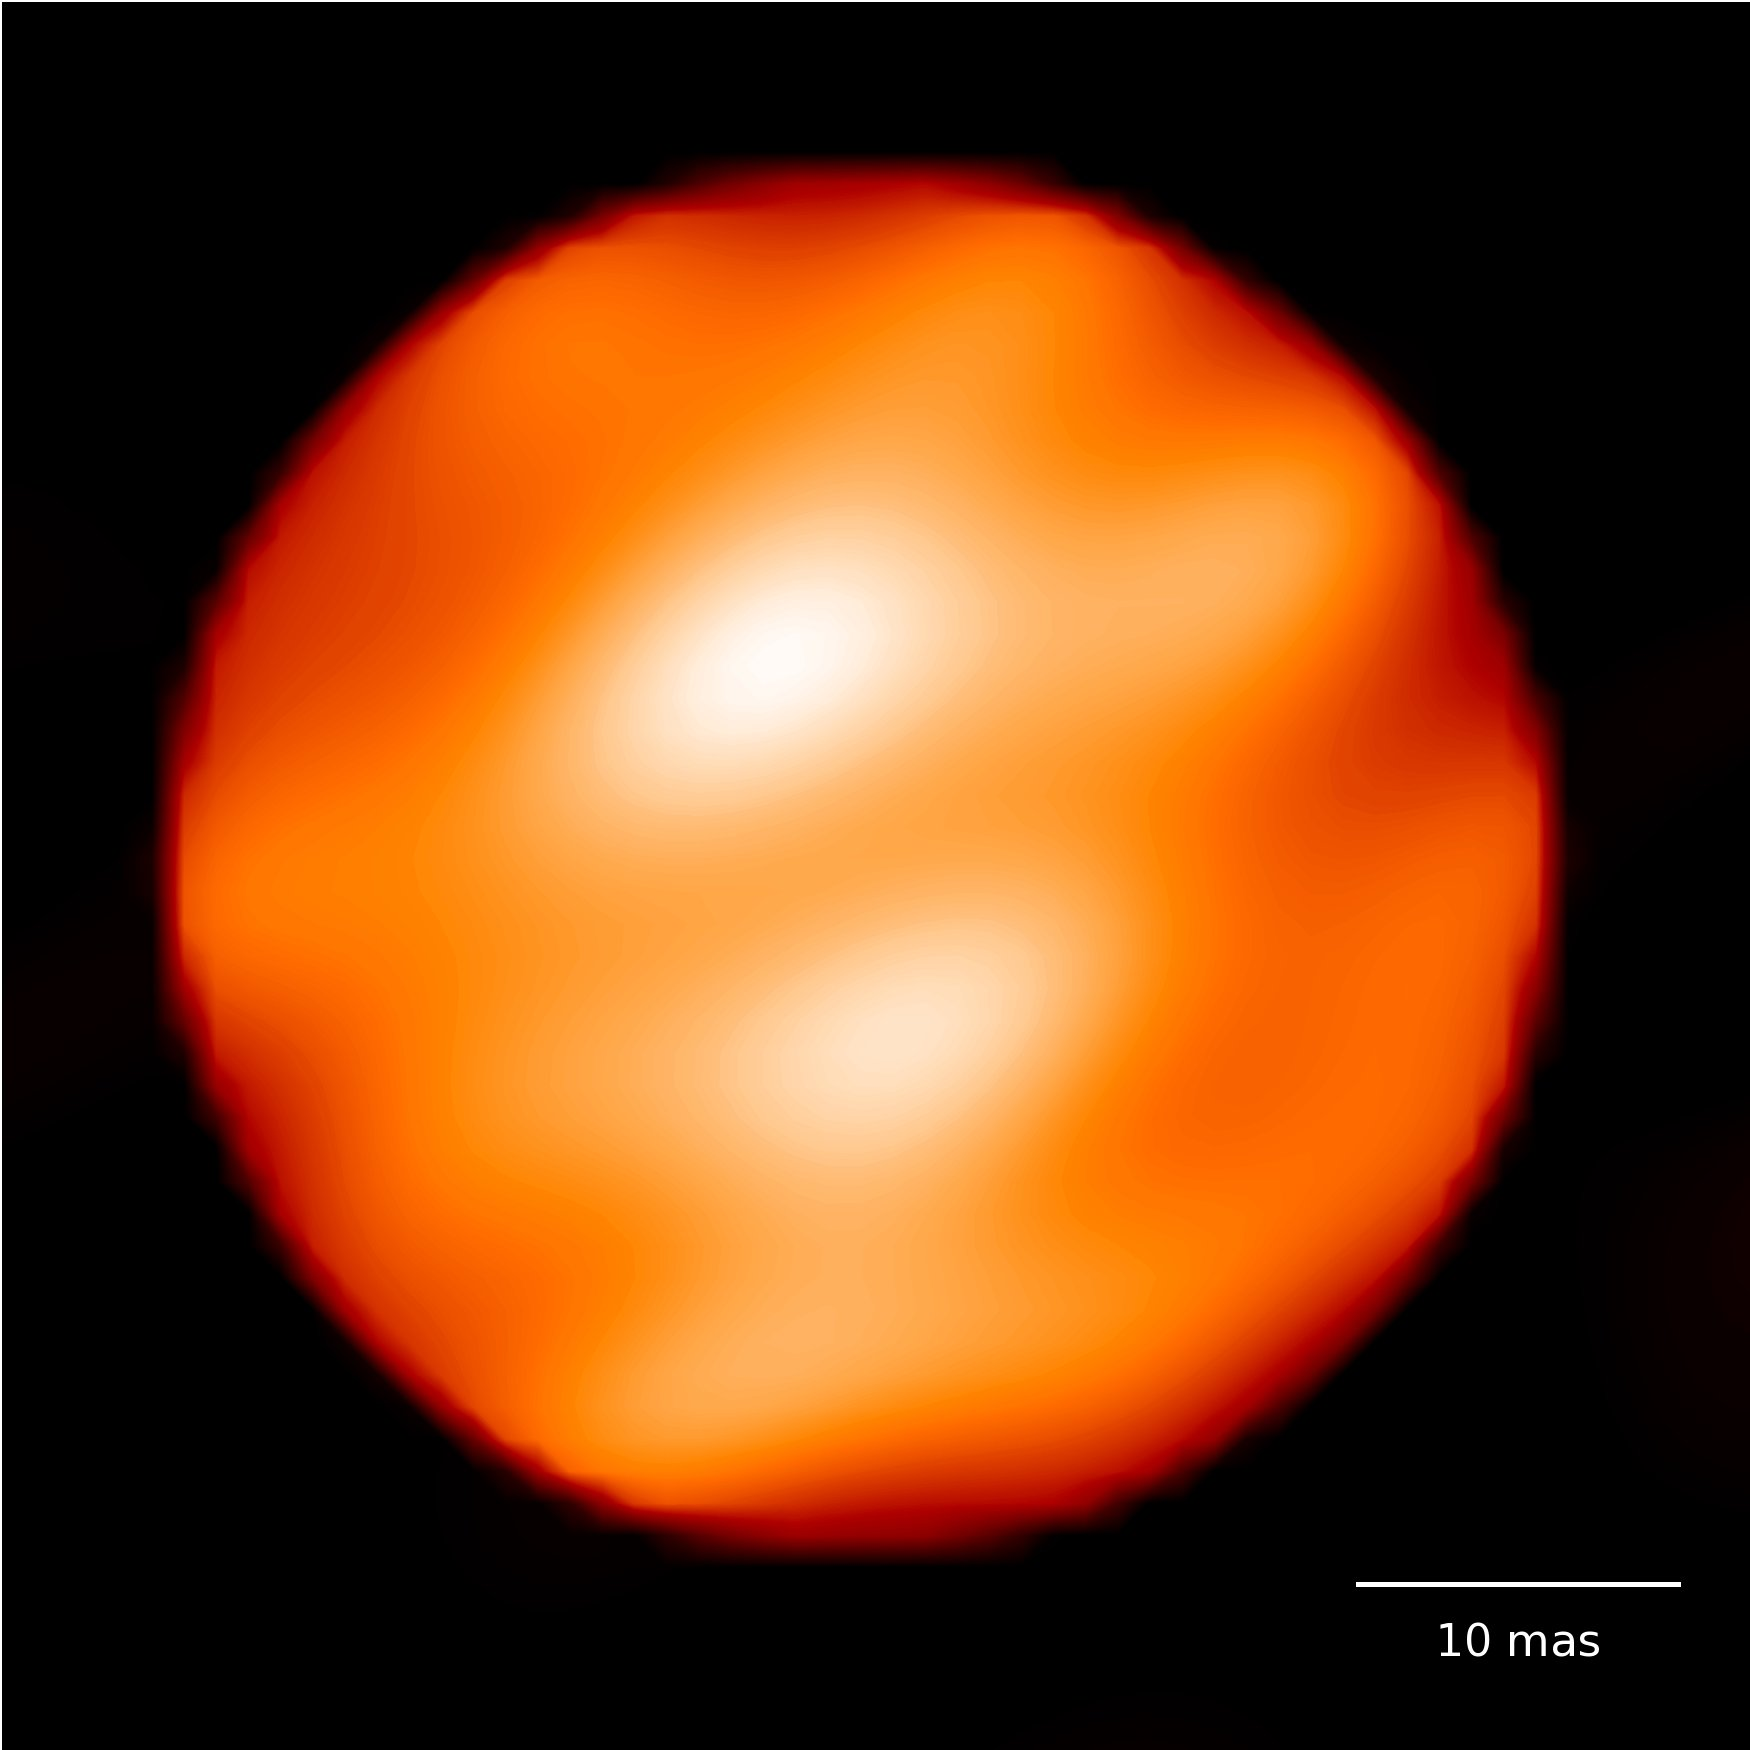
\includegraphics[width=\linewidth]{Betel_haubois}
\caption[Betelgeuse]{\label{f.betelgeuse} A reconstructed image of Betelgeuse made using interferometry. \imgcred\ Xavier Haubois et al. (Observatoire de Paris)}
\end{marginfigure}
The best-known example of an evolved massive star is Betelgeuse, which is large enough and close enough to be resolved (Fig.~\ref{f.betelgeuse} shows a reconstructed image made with interferometry). Betelgeuse probably started as a blue main-sequence star of approximately $\val{20}{\Msun}$ and is now burning helium in its core now. The extended envelope, $\approx\val{5}{\AU}$ in radius, has large convective cells (bright spots in image) and pulsates violently. As can be inferred from Table~\ref{t.burning-timescales}, in less than $\val{1}{\Mega\yr}$ Betelgeuse's core will reach nuclear statistical equilibrium; no more nuclear energy will be available and Betelgeuse will transform into either a neutron star or black hole, as we describe next.

\subsection{Core collapse}
When the core of a massive star reaches nuclear statistical equilibrium, there are no further sources of energy available. Fusion reactions in the shells surrounding the core add mass to it, causing it to contract. The increasing density raises the electron Fermi energy. When the Fermi energy approaches the rest mass of the electrons---$m_{e}c^{2} = \val{0.511}{\MeV}$---the electrons move relativistically. This dramatically alters the equation of state.

A particle's energy, including rest mass, is
\[
	E = \sqrt{p^{2}c^{2} + m^{2}c^{4}} = mc^{2}\left[1 + \left(\frac{p}{mc}\right)^{2}\right]^{1/2};
\]
when $p\ll mc$, we can expand this as $E\approx m c^{2} + p^{2}/2m$---that is, as the sum of the rest mass and the Newtonian kinetic energy. In the opposite limit, when $p \gg mc$, $E \approx pc$. Let's see how this relativistic limit affects the degenerate equation of state. Recall that we fill energy states, starting with the lowest open levels until we have added all $N$ electrons (eq.~[\ref{e.number-degenerate}]):
\[
	N = \frac{2}{h^{3}}\int_{V}\dif^{3}x\int_{0}^{\EF}\dif^{3}p.
\]
Change variables, $\dif^{3}p = 4\pi p^{2}\,\dif p = 4\pi c^{-3}\varepsilon^{2}\,\dif\varepsilon$, where $\varepsilon = pc$ is the energy of a single, relativistic electron:
\[
	N = \frac{8\pi}{h^{3}c^{3}}V \int_{0}^{\EF} \varepsilon^{2}\,\dif\varepsilon
	= \frac{8\pi}{3h^{3}c^{3}} V  \EF^{3}.
\]
This gives the Fermi energy,
\[
	\EF = hc\left(\frac{3}{8\pi}\frac{N}{V}\right)^{1/3}.
\]
To get the total energy, multiply each electron by its energy $\varepsilon$ and integrate over phase space:
\[
	E = \frac{8\pi}{h^{3}c^{3}}V\int_{0}^{\EF}\varepsilon^{3}\,\dif\varepsilon = 
		\frac{1}{4}\frac{8\pi}{h^{3}c^{3}}V\EF^{4} = \frac{3}{4}N\EF.
\]
For a relativistic gas, the pressure is $P = (1/3)(E/V)$ (cf.\ Box~\ref{sb.radiation-pressure}), so that
\begin{equation}
\label{e.pressure-relativistic}
	P = \frac{1}{4}n\EF = \frac{1}{4}\left(\frac{3}{8\pi}\right)^{1/3}hc n^{4/3},
\end{equation}
with $n = \rho/\mu_{e}m_{u}$. Instead of $P\propto\rho^{5/3}$, as for a non-relativistic gas, $P\propto\rho^{4/3}$.

\subsection{The Chandrasekhar mass}

In exercise~\ref{ex.degenerate-mass-radius}, we constructed a mass-radius relation for white dwarfs by combining the virial relations,
\begin{eqnarray*}
   P    &\propto& \frac{GM^{2}}{R^{4}}\\
   \rho &\propto& \frac{M}{R^{3}}
\end{eqnarray*}
and the equation of state for a non-relativistic, degenerate, ideal gas.  We found that $R\propto M^{-1/3}$.  If we try that with our relativistic equation of state, eq.~(\ref{e.pressure-relativistic}), we get
\[
	\frac{GM^{2}}{R^{4}} \propto P = \frac{1}{4}\left(\frac{3}{8\pi}\right)^{1/3}hc\; \left(\frac{\rho}{\mb\mu_{e}}\right)^{4/3} \propto \frac{hc}{\mb^{4/3}}\frac{M^{4/3}}{R^{4}}.
\]
The radius $R$ cancels, and what we have is a relation $M\propto (hc/G)^{3/2}/\mb^{2}$.  This is rather odd: a gas with a relativistic equation of state in hydrostatic balance has a characteristic mass defined in terms of fundamental constants.

Let's investigate this further. Suppose we have a box with adjustable sides, which we pack with $N$ degenerate electrons. We add some nuclei for mass, so that the total mass in the box is $\mu_{e}\mb N$. The volume of the box $V \sim R^{3}$, and since the electrons are degenerate, the volume per electron is roughly $\lambda^{3}$, where $\lambda \sim h/p$ is the wavelength of the electrons.  As a result, $N = (R/\lambda)^{3}$; further, the momentum of an electron is
\[	p \sim \frac{h}{\lambda} \sim h\frac{N^{1/3}}{R}. \]
If our electrons were non-relativistic, the total, kinetic plus gravitational, energy of our box would be
\[
	E_{\mathrm{total}} = N\frac{p^{2}}{2m_{e}} - \frac{GM^{2}}{R} \sim N^{5/3}\frac{h^{2}}{R^{2}m_{e}} - GN^{2}\mu_{e}^{2}\mb^{2} \frac{1}{R}.
\]
For a given $N$, we can adjust $R$ to make $E_{\mathrm{total}}<0$, and indeed, if we satisfy the virial theorem, we will recover the $R\propto M^{-1/3}$ scaling.

If, however, the electrons are relativistic then the total energy is
\begin{eqnarray*}
	E_{\mathrm{total}} = Npc - \frac{GM^{2}}{R} 
		&=& \frac{1}{R}\left[hc N^{4/3} - G N^{2}(\mu_{e}\mb)^{2}\right]\\
		&=& G(\mu_{e}\mb)^{2}\frac{N^{4/3}}{R}
		{\color{red}\left[ \frac{hc}{G(\mu_{e}\mb)^{2}} - N^{2/3}\right]}.
\end{eqnarray*}
Look at the term in $\color{red}\left[\cdot\right]$.
If $N < [hc/G/(\mu_{e}\mb)^{2}]^{3/2}$, then $E_{\mathrm{total}} > 0$; by making $R$ larger, however, we can lower the energy until the electrons are no longer relativistic, and then we can again recover the virial scaling.  If $N > [hc/G(\mu_{e}\mb)^{2}]^{3/2}$ then $E_{\mathrm{total}} < 0$; by making $R$ smaller, however, we can keep reducing $E_{\mathrm{total}}$ indefinitely. 
\begin{quote}\itshape
There is no bound state with finite $R$ for $M>(hc/G)^{3/2}(\mu_{e}\mb)^{-2}$.
\end{quote}

\begin{sidebar}[Instability for a relativistic equation of state]
There is another way of looking at the onset of instability which is instructive (this treatment follows that in \citet{Cox1980Theory-of-Stell}). In exercise \ref{ex.stellar-oscillation-period} you found that during a contraction or expansion, the equation of motion for a thin layer at the star's surface was
\[
	\ddot{\delta R} = \frac{GM}{R^{2}}\left[4-3\gamma\right]\frac{\delta R}{R}.
\]
Here $M$ and $R$ are the total stellar mass and radius, and the adiabatic pressure-density relation is $P\propto \rho^{\gamma}$.

For a non-relativistic gas with $\gamma = 5/3$, we have $\ddot{\delta R} \propto -\delta R$: the star oscillates with a period that is comparable to the dynamical timescale of the star. If, however, $\gamma < 4/3$ the equation of motion is $\ddot{\delta R} \propto \delta R$, which has an exponential solution: squeeze the star slightly, and it will implode!

Let's work out a more physical explanation for what is happening. Suppose we have a star in virial equilibrium, with a the central pressure and density
\begin{eqnarray*}
P &\propto& \frac{GM^{2}}{R^{4}} \\
\rho &\propto& \frac{M}{R^{3}}.
\end{eqnarray*}
Now if we contract the star by a small amount, say $\delta R/R = -1\%$, then the density increases by an amount $\delta\rho/\rho = -3\delta R/R = 3\%$. How does the pressure respond? If the star contracts slowly, on a Kelvin-Helmholtz timescale, then there is time for heat to radiate away, so that the internal pressure can increase by the amount needed to maintain virial equilibrium: in this case $\delta P/P = -4\delta R/R = 4\%$. Under an \emph{adiabatic} contraction, however, there is not enough time for the star to radiate away excess heat; as a consequence, the pressure and density are linked, so that $\delta P/P = \gamma\delta \rho/\rho = -3\gamma\delta R/R$.

If the adiabatic index is $\gamma = 4/3$, then during an adiabatic compression of $\delta R/R = -1\%$, the density increases by $3|\delta R/R| = 3\%$ and the pressure increases by $3\gamma|\delta R/R| = 4\%$, which is precisely the increase needed to maintain mechanical equilibrium. As a result, the star remains in hydrostatic balance at its new, smaller radius. This is why there was no mass-radius relation for $\gamma = 4/3$; it takes no energy to contract (or expand) the star.

For $\gamma > 4/3$, the central pressure increases during contraction by $3\gamma|\delta R/R| > 4|\delta R/R|$. As a result, the pressure becomes greater than the amount needed for hydrostatic balance. This excess pressure pushes the star outward and acts as a restoring source. During an expansion, the pressure falls below the amount needed for hydrostatic equilibrium, so gravity halts the expansion and forces the star to contract. Hence, for $\gamma > 4/3$, the star responds to a radial perturbation by oscillating with a period comparable to the dynamical timescale (cf.\ exercise \ref{ex.stellar-oscillation-period}).

In contrast, if $\gamma < 4/3$ the increase in pressure during contraction is $3\gamma|\delta R/R| < 4|\delta R/R|$. The gas pressure does not increase enough to maintain hydrostatic equilibrium, and so the star's contraction accelerates. A small perturbation inwards leads to implosion.
\end{sidebar}

Thus, there is a limit to the total mass that can be supported in hydrostatic equilibrium by degenerate electrons. 
An exact calculation for the maximum mass of a cold, degenerate star yields
\begin{equation}\label{e.Chandrasekhar}
	M_{\mathrm{Ch}} = 1.456 \left(\frac{2}{\mu_{e}}\right)^{2}\Msun.
\end{equation}
When the mass reaches this limiting value, known as the \newterm{Chandrasekhar mass}\sidenote{Derived by S. Chandrasekhar at age 20(!) while traveling from India to England in 1930}, the electrons become relativistic and $\partial P/\partial \rho \to 4/3$; the star becomes unstable and collapses.

When the core of a massive star begins its collapse, the electron Fermi is $\sim\MeV$, which is sufficient to induce electron captures on iron-group nuclei. These captures increase $\mu_{e}$ and reduce $M_{\mathrm{Ch}}$. As the core begins the final plunge, the rapidly rising temperature induces the photodissociation of iron-group nuclei into neutrons, protons, and helium nuclei. This process is endothermic, which further robs the core of pressure support and accelerates the collapse. The effective $\gamma = \partial P/\partial\rho < 4/3$ on account of the photodissociation and electron captures, and the core implodes.

As the core density approaches $\val{0.16}{\fermi^{-3}}$,\marginnote{the density of an atomic nucleus} the nucleons begin to repel one another on account of the strong nuclear force. This abruptly halts the collapse and launches a shockwave outwards. The core now consists mostly of neutrons and is termed a \newterm{neutron star}.

\begin{exercisebox}[Gravitational binding energy of a neutron star]
What is the mass density if the number density of nucleons is $\val{0.16}{\fermi^{-3}}$? What is the gravitational binding energy for an object with a mass \val{1.4}{\Msun} at this density?
\end{exercisebox}

The outward traveling shockwave soon stalls as the outer layers of the star fall inward. The energy needed to blow the envelope off is about 1\% of the gravitational binding energy of the core, so there is plenty of energy available to disperse the envelope if this energy can be tapped. Most of the gravitational binding energy released by the imploding core is carried outwards by neutrinos. 
During the collapse, the neutrino mean free path becomes smaller than the core radius for two reasons: the weak interaction cross-section increases as the nucleons reach temperatures $\gtrsim\val{10^{10}}{\K}$, and the mean free path $\ell = (n\sigma)^{-1}$ decreases with density. 
As a result the neutrinos become trapped and must diffuse of the collapsing core. As the neutrinos diffuse out, they transfer a small fraction of their energy to the material heating it. This tends to push the shock outward. A competition arises between the ram pressure of infalling matter and the heating from the neutrinos. If the neutrinos can transfer enough energy to the envelope, then the envelope will be blown off in a supernova. If not, then matter will continue to accumulate onto the neutron star. The maximum mass of a neutron star is uncertain\sidenote{By timing pulsars in a binary system, the orbital parameters and hence the mass of the neutron star can be deduced; the largest measured mass is \val{2}{\Msun}.}, but on physical grounds is likely $< \val{3}{\Msun}$. If the shock is not re-energized, then conceivably the entire star could implode into a black hole.

\section{Stellar resurrection}
\label{s.stellar-resurrection}

In the previous section, we learned that stars with $M\lesssim\valrng[--]{8}{10}{\Msun}$ eventually become white dwarfs composed of carbon and oxygen and supported by electron degeneracy pressure; and that more massive stars have cores that collapse, either to form neutron stars supported by the strong nuclear interaction or to collapse fully into black holes.

Both the white dwarfs and neutron stars that emerge from the ashes of isolated stars slowly cool and dim. The cooling of white dwarfs can be modeled accurately enough that observations of white dwarfs in clusters can be used to infer the ages of and distances to their host clusters. No such capability is possible with isolated neutron stars: most are too dim to be observed, and there are vast uncertainties about the composition of the deep interior, where the density is several times higher than that of an atomic nucleus. Rather, efforts have been on using observations of the handful of isolated neutron stars with measured surface temperatures to constrain models of nuclear matter.

Many observed neutron stars are endowed with strong magnetic field $\gtrsim\val{10^{8}}{\unitstyle{T}}$. If the neutron star spins rapidly enough, then a tremendous voltage is generated is the surface that accelerates charges above the polar caps. In turn, these accelerated charges emit photons that fan outward from the poles. As the neutron star spins, the beams of radiation are swept around; a distant observer therefore observes light pulsing at the rotation frequency of the star.\marginnote[-4\baselineskip]{Interestingly, the radio emission from several pulsars, including the Crab, was independently detected by Airman C. Schisler at the Ballistic Missile Early Warning Site, Clear Air Force Station, Alaska.} These systems, known as \newterm{pulsars}, were discovered\cite{Hewish1968Observation-of-} by Jocelyn Bell and Anthony Hewish in 1967.

\begin{exercisebox}[Limiting spin frequency]
The Crab pulsar pulsates at a frequency of \val{33}{\Hz}. For a star of \val{1}{\Msun}, find the maximum radius such that material at the equator remains bound to the star. Based on these results, argue that the Crab pulsar cannot be a white dwarf.
\end{exercisebox}

\newthought{Many stars are in binary systems.} If the binary happens to survive the evolution off the main sequence, it can often happen that the orbit is close enough for matter to be tidally stripped from the companion and \newterm{accreted} onto the compact star (i.e., white dwarf, neutron star, or black hole). As matter falls into the gravitational potential, it liberates a considerable amount of energy. This makes the system bright.

\begin{exercisebox}[Accretion onto a neutron star]
Let's estimate the luminosity and surface temperature of an accreting neutron star. Assume a mass of \val{1.4}{\Msun} and a radius of \val{10}{\kilo\meter}. How much gravitational energy (in MeV) is released when a proton falls onto the surface (use a Newtonian approximation for the gravitational potential). How does this compare to the energy released (per proton) from the fusion of hydrogen into helium? Now suppose the neutron star is accreting at \val{10^{17}}{\gram\usk\second^{-1}}, which is a typical rate for many observed systems. What would be the luminosity generated by this accretion? Suppose the luminosity were emitted thermally from the surface of the neutron star. What would be the surface effective temperature? In what band (e.g., visible, IR, UV, X-ray) would you want to observe this system?
\end{exercisebox}

When sufficient material\sidenote{The accreted matter is usually mostly hydrogen, but if the companion star is evolved it could be enriched in helium or even, if the companion star is itself a white dwarf, carbon and oxygen.} has accumulated on the surface, thermonuclear reactions can ignite in the accreted layer. This ignition is typically thermally unstable and leads to an explosion. On a white dwarf, this explosion is manifest as a \newterm{nova}\sidenote{from the Latin \emph{novus} meaning ``new''} as the white dwarf abruptly brightens and then dims over several weeks to months. The mass of the burning layer is typically \valrng{10^{-5}}{10^{-4}}{\Msun}; at typical accretion rates $\lesssim\val{10^{-9}}{\Msun\usk\yr^{-1}}$ the time between the explosions is thousands of years or longer. The amount of mass necessary for ignition decreases strongly with the mass of the white dwarf, however, so that the time between explosions can be years to decades. In these systems the novae are observed to reoccur and they are called---appropriately enough---\newterm{recurrent novae}.
On a neutron star, the explosion is observed as an \newterm{X-ray burst} that lasts \valrng[--]{10}{100}{\second}. The strong gravity means the amount of material needed for ignition is much less than on a white dwarf: roughly \val{10^{-12}}{\Msun}. As a consequence, the time between bursts can be as short as hours to days. 



\backmatter
\bibliographystyle{plainnat}
\bibliography{bibs/stellar-astro}

\end{document}
